%!TEX TS-program = xelatex
%!TEX encoding = UTF-8 Unicode
%times,


%%%%%%%%%%%%%%%%%%%%%%%%%%%%%%%%%%%%%%%%%
% The Legrand Orange Book
% LaTeX Template
% Version 2.0 (9/2/15)
%
% This template has been downloaded from:
% http://www.LaTeXTemplates.com
% License:
% CC BY-NC-SA 3.0 (http://creativecommons.org/licenses/by-nc-sa/3.0/)
% Important note:
% Chapter heading images should have a 2:1 width:height ratio,
% e.g. 920px width and 460px height.
%%%%%%%%%%%%%%%%%%%%%%%%%%%%%%%%%%%%%%%%%

\documentclass[11pt,fleqn,twoside]{book}
\makeatletter
\usepackage{indentfirst}
\usepackage{xeCJK}
\usepackage{cancel}
\setCJKmainfont[BoldFont={SimHei},ItalicFont={KaiTi}]{SimSun}
\usepackage{bm}
\usepackage{amssymb}
\usepackage{mathrsfs}
\usepackage[squaren]{SIunits}
\usepackage{ulem}
\usepackage[version=3]{mhchem}
\usepackage{draftwatermark}
\SetWatermarkText{\textsc{Draft Translation}}
\SetWatermarkLightness{0.88}
\SetWatermarkScale{0.4}
\usepackage{setspace}
\usepackage{marginfix}
%\include{marginpar}
%%%%%%%%%%%%%%%%%%%%%%%%%%%%%%%%%%%%%%%%%
% The Legrand Orange Book
% Structural Definitions File
% Version 2.0 (9/2/15)
%
% Original author:
% Mathias Legrand (legrand.mathias@gmail.com) with modifications by:
% Vel (vel@latextemplates.com)
% 
% This file has been downloaded from:
% http://www.LaTeXTemplates.com
%
% License:
% CC BY-NC-SA 3.0 (http://creativecommons.org/licenses/by-nc-sa/3.0/)
%
%%%%%%%%%%%%%%%%%%%%%%%%%%%%%%%%%%%%%%%%%

%----------------------------------------------------------------------------------------
%	VARIOUS REQUIRED PACKAGES AND CONFIGURATIONS
%----------------------------------------------------------------------------------------

\usepackage[top=3cm,bottom=3cm,left=3cm,right=3cm,headsep=10pt,a4paper,outer=7cm,marginparwidth=4cm, marginparsep=2cm]{geometry} % Page margins

\usepackage{graphicx} % Required for including pictures
\graphicspath{{Pictures/}} % Specifies the directory where pictures are stored

\usepackage{lipsum} % Inserts dummy text

\usepackage{tikz} % Required for drawing custom shapes

\usepackage[english]{babel} % English language/hyphenation

\usepackage{enumitem} % Customize lists
\setlist{nolistsep} % Reduce spacing between bullet points and numbered lists

\usepackage{booktabs} % Required for nicer horizontal rules in tables

\usepackage{xcolor} % Required for specifying colors by name
\definecolor{ocre}{RGB}{243,102,25} % Define the orange color used for highlighting throughout the book

%----------------------------------------------------------------------------------------
%	FONTS
%----------------------------------------------------------------------------------------

\usepackage{avant} % Use the Avantgarde font for headings
%\usepackage{times} % Use the Times font for headings
%\usepackage{mathptmx} % Use the Adobe Times Roman as the default text font together with math symbols from the Sym­bol, Chancery and Com­puter Modern fonts

%\usepackage{microtype} % Slightly tweak font spacing for aesthetics
\usepackage[utf8]{inputenc} % Required for including letters with accents
\usepackage[T1]{fontenc} % Use 8-bit encoding that has 256 glyphs

%----------------------------------------------------------------------------------------
%	BIBLIOGRAPHY AND INDEX
%----------------------------------------------------------------------------------------

%\usepackage[style=alphabetic,citestyle=numeric,sorting=nyt,sortcites=true,autopunct=true,babel=hyphen,hyperref=true,abbreviate=false,backref=true,backend=biber]{biblatex}
%\addbibresource{bibliography.bib} % BibTeX bibliography file
%\defbibheading{bibempty}{}

\usepackage{calc} % For simpler calculation - used for spacing the index letter headings correctly
\usepackage{makeidx} % Required to make an index
\makeindex % Tells LaTeX to create the files required for indexing

%----------------------------------------------------------------------------------------
%	MAIN TABLE OF CONTENTS
%----------------------------------------------------------------------------------------

\usepackage{titletoc} % Required for manipulating the table of contents

\contentsmargin{0cm} % Removes the default margin

% Part text styling
\titlecontents{part}[0cm]
{\addvspace{20pt}\centering\large\bfseries}
{}
{}
{}

% Chapter text styling
\titlecontents{chapter}[1.25cm] % Indentation
{\addvspace{12pt}\large\sffamily\bfseries} % Spacing and font options for chapters
{\color{ocre!60}\contentslabel[\Large\thecontentslabel]{1.25cm}\color{ocre}} % Chapter number
{\color{ocre}}  
{\color{ocre!60}\normalsize\;\titlerule*[.5pc]{.}\;\thecontentspage} % Page number

% Section text styling
\titlecontents{section}[1.25cm] % Indentation
{\addvspace{3pt}\sffamily\bfseries} % Spacing and font options for sections
{\contentslabel[\thecontentslabel]{1.25cm}} % Section number
{}
{\hfill\color{black}\thecontentspage} % Page number
[]

% Subsection text styling
\titlecontents{subsection}[1.25cm] % Indentation
{\addvspace{1pt}\sffamily\small} % Spacing and font options for subsections
{\contentslabel[\thecontentslabel]{1.25cm}} % Subsection number
{}
{\ \titlerule*[.5pc]{.}\;\thecontentspage} % Page number
[]

% List of figures
\titlecontents{figure}[0em]
{\addvspace{-5pt}\sffamily}
{\thecontentslabel\hspace*{1em}}
{}
{\ \titlerule*[.5pc]{.}\;\thecontentspage}
[]

% List of tables
\titlecontents{table}[0em]
{\addvspace{-5pt}\sffamily}
{\thecontentslabel\hspace*{1em}}
{}
{\ \titlerule*[.5pc]{.}\;\thecontentspage}
[]

%----------------------------------------------------------------------------------------
%	MINI TABLE OF CONTENTS IN PART HEADS
%----------------------------------------------------------------------------------------

% Chapter text styling
\titlecontents{lchapter}[0em] % Indenting
{\addvspace{15pt}\large\sffamily\bfseries} % Spacing and font options for chapters
{\color{ocre}\contentslabel[\Large\thecontentslabel]{1.25cm}\color{ocre}} % Chapter number
{}  
{\color{ocre}\normalsize\sffamily\bfseries\;\titlerule*[.5pc]{.}\;\thecontentspage} % Page number

% Section text styling
\titlecontents{lsection}[0em] % Indenting
{\sffamily\small} % Spacing and font options for sections
{\contentslabel[\thecontentslabel]{1.25cm}} % Section number
{}
{}

% Subsection text styling
\titlecontents{lsubsection}[.5em] % Indentation
{\normalfont\footnotesize\sffamily} % Font settings
{}
{}
{}

%----------------------------------------------------------------------------------------
%	PAGE HEADERS
%----------------------------------------------------------------------------------------

\usepackage{fancyhdr} % Required for header and footer configuration

\pagestyle{fancy}
\renewcommand{\chaptermark}[1]{\markboth{\sffamily\normalsize\bfseries\chaptername\ \thechapter.\ #1}{}} % Chapter text font settings
\renewcommand{\sectionmark}[1]{\markright{\sffamily\normalsize\thesection\hspace{5pt}#1}{}} % Section text font settings
\fancyhf{} \fancyhead[LE,RO]{\sffamily\normalsize\thepage} % Font setting for the page number in the header
\fancyhead[LO]{\rightmark} % Print the nearest section name on the left side of odd pages
\fancyhead[RE]{\leftmark} % Print the current chapter name on the right side of even pages
\renewcommand{\headrulewidth}{0.5pt} % Width of the rule under the header
\addtolength{\headheight}{2.5pt} % Increase the spacing around the header slightly
\renewcommand{\footrulewidth}{0pt} % Removes the rule in the footer
\fancypagestyle{plain}{\fancyhead{}\renewcommand{\headrulewidth}{0pt}} % Style for when a plain pagestyle is specified

% Removes the header from odd empty pages at the end of chapters
\makeatletter
\renewcommand{\cleardoublepage}{
\clearpage\ifodd\c@page\else
\hbox{}
\vspace*{\fill}
\thispagestyle{empty}
\newpage
\fi}

%----------------------------------------------------------------------------------------
%	THEOREM STYLES
%----------------------------------------------------------------------------------------

\usepackage{amsmath,amsfonts,amssymb,amsthm} % For math equations, theorems, symbols, etc

\newcommand{\intoo}[2]{\mathopen{]}#1\,;#2\mathclose{[}}
\newcommand{\ud}{\mathop{\mathrm{{}d}}\mathopen{}}
\newcommand{\intff}[2]{\mathopen{[}#1\,;#2\mathclose{]}}
\newtheorem{notation}{Notation}[chapter]

% Boxed/framed environments
\newtheoremstyle{ocrenumbox}% % Theorem style name
{0pt}% Space above
{0pt}% Space below
{\normalfont}% % Body font
{}% Indent amount
{\small\bf\sffamily\color{ocre}}% % Theorem head font
{\;}% Punctuation after theorem head
{0.25em}% Space after theorem head
{\small\sffamily\color{ocre}\thmname{#1}\nobreakspace\thmnumber{\@ifnotempty{#1}{}\@upn{#2}}% Theorem text (e.g. Theorem 2.1)
\thmnote{\nobreakspace\the\thm@notefont\sffamily\bfseries\color{black}---\nobreakspace#3.}} % Optional theorem note
\renewcommand{\qedsymbol}{$\blacksquare$}% Optional qed square

\newtheoremstyle{blacknumex}% Theorem style name
{5pt}% Space above
{5pt}% Space below
{\normalfont}% Body font
{} % Indent amount
{\small\bf\sffamily}% Theorem head font
{\;}% Punctuation after theorem head
{0.25em}% Space after theorem head
{\small\sffamily{\tiny\ensuremath{\blacksquare}}\nobreakspace\thmname{#1}\nobreakspace\thmnumber{\@ifnotempty{#1}{}\@upn{#2}}% Theorem text (e.g. Theorem 2.1)
\thmnote{\nobreakspace\the\thm@notefont\sffamily\bfseries---\nobreakspace#3.}}% Optional theorem note

\newtheoremstyle{blacknumbox} % Theorem style name
{0pt}% Space above
{0pt}% Space below
{\normalfont}% Body font
{}% Indent amount
{\small\bf\sffamily}% Theorem head font
{\;}% Punctuation after theorem head
{0.25em}% Space after theorem head
{\small\sffamily\thmname{#1}\nobreakspace\thmnumber{\@ifnotempty{#1}{}\@upn{#2}}% Theorem text (e.g. Theorem 2.1)
\thmnote{\nobreakspace\the\thm@notefont\sffamily\bfseries---\nobreakspace#3.}}% Optional theorem note

% Non-boxed/non-framed environments
\newtheoremstyle{ocrenum}% % Theorem style name
{5pt}% Space above
{5pt}% Space below
{\normalfont}% % Body font
{}% Indent amount
{\small\bf\sffamily\color{ocre}}% % Theorem head font
{\;}% Punctuation after theorem head
{0.25em}% Space after theorem head
{\small\sffamily\color{ocre}\thmname{#1}\nobreakspace\thmnumber{\@ifnotempty{#1}{}\@upn{#2}}% Theorem text (e.g. Theorem 2.1)
\thmnote{\nobreakspace\the\thm@notefont\sffamily\bfseries\color{black}---\nobreakspace#3.}} % Optional theorem note
\renewcommand{\qedsymbol}{$\blacksquare$}% Optional qed square
\makeatother

% Defines the theorem text style for each type of theorem to one of the three styles above
\newcounter{dummy} 
\numberwithin{dummy}{section}
\theoremstyle{ocrenumbox}
\newtheorem{theoremeT}[dummy]{Theorem}
\newtheorem{problem}{Problem}[chapter]
\newtheorem{exerciseT}{Exercise}[chapter]
\theoremstyle{blacknumex}
\newtheorem{exampleT}{Example}[chapter]
\theoremstyle{blacknumbox}
\newtheorem{vocabulary}{Vocabulary}[chapter]
\newtheorem{definitionT}{Definition}[]
\newtheorem{corollaryT}[dummy]{Corollary}
\theoremstyle{ocrenum}
\newtheorem{proposition}[dummy]{Proposition}

%----------------------------------------------------------------------------------------
%	DEFINITION OF COLORED BOXES
%----------------------------------------------------------------------------------------

\RequirePackage[framemethod=default]{mdframed} % Required for creating the theorem, definition, exercise and corollary boxes

% Theorem box
\newmdenv[skipabove=7pt,
skipbelow=7pt,
backgroundcolor=black!5,
linecolor=ocre,
innerleftmargin=5pt,
innerrightmargin=5pt,
innertopmargin=5pt,
leftmargin=0cm,
rightmargin=0cm,
innerbottommargin=5pt]{tBox}

% Exercise box	  
\newmdenv[skipabove=7pt,
skipbelow=7pt,
rightline=false,
leftline=true,
topline=false,
bottomline=false,
backgroundcolor=ocre!10,
linecolor=ocre,
innerleftmargin=5pt,
innerrightmargin=5pt,
innertopmargin=5pt,
innerbottommargin=5pt,
leftmargin=0cm,
rightmargin=0cm,
linewidth=4pt]{eBox}	

% Definition box
\newmdenv[skipabove=7pt,
skipbelow=7pt,
rightline=false,
leftline=true,
topline=false,
bottomline=false,
linecolor=ocre,
innerleftmargin=5pt,
innerrightmargin=5pt,
innertopmargin=0pt,
leftmargin=0cm,
rightmargin=0cm,
linewidth=4pt,
innerbottommargin=0pt]{dBox}	

% Corollary box
\newmdenv[skipabove=7pt,
skipbelow=7pt,
rightline=false,
leftline=true,
topline=false,
bottomline=false,
linecolor=gray,
backgroundcolor=black!5,
innerleftmargin=5pt,
innerrightmargin=5pt,
innertopmargin=5pt,
leftmargin=0cm,
rightmargin=0cm,
linewidth=4pt,
innerbottommargin=5pt]{cBox}

% Creates an environment for each type of theorem and assigns it a theorem text style from the "Theorem Styles" section above and a colored box from above
\newenvironment{theorem}{\begin{tBox}\begin{theoremeT}}{\end{theoremeT}\end{tBox}}
\newenvironment{exercise}{\begin{eBox}\begin{exerciseT}}{\hfill{\color{ocre}\tiny\ensuremath{\blacksquare}}\end{exerciseT}\end{eBox}}				  
\newenvironment{definition}{\begin{dBox}\begin{definitionT}}{\end{definitionT}\end{dBox}}	
\newenvironment{example}{\begin{exampleT}}{\hfill{\tiny\ensuremath{\blacksquare}}\end{exampleT}}		
\newenvironment{corollary}{\begin{cBox}\begin{corollaryT}}{\end{corollaryT}\end{cBox}}	

%----------------------------------------------------------------------------------------
%	REMARK ENVIRONMENT
%----------------------------------------------------------------------------------------

\newenvironment{remark}{\par\vspace{10pt}\small % Vertical white space above the remark and smaller font size
\begin{list}{}{
\leftmargin=35pt % Indentation on the left
\rightmargin=25pt}\item\ignorespaces % Indentation on the right
\makebox[-2.5pt]{\begin{tikzpicture}[overlay]
\node[draw=ocre!60,line width=1pt,circle,fill=ocre!25,font=\sffamily\bfseries,inner sep=2pt,outer sep=0pt] at (-15pt,0pt){\textcolor{ocre}{R}};\end{tikzpicture}} % Orange R in a circle
\advance\baselineskip -1pt}{\end{list}\vskip5pt} % Tighter line spacing and white space after remark

%----------------------------------------------------------------------------------------
%	SECTION NUMBERING IN THE MARGIN
%----------------------------------------------------------------------------------------

\makeatletter
\renewcommand{\@seccntformat}[1]{\llap{\textcolor{ocre}{\csname the#1\endcsname}\hspace{1em}}}                    
\renewcommand{\section}{\@startsection{section}{1}{\z@}
{-4ex \@plus -1ex \@minus -.4ex}
{1ex \@plus.2ex }
{\normalfont\large\sffamily\bfseries}}
\renewcommand{\subsection}{\@startsection {subsection}{2}{\z@}
{-3ex \@plus -0.1ex \@minus -.4ex}
{0.5ex \@plus.2ex }
{\normalfont\sffamily\bfseries}}
\renewcommand{\subsubsection}{\@startsection {subsubsection}{3}{\z@}
{-2ex \@plus -0.1ex \@minus -.2ex}
{.2ex \@plus.2ex }
{\normalfont\small\sffamily\bfseries}}                        
\renewcommand\paragraph{\@startsection{paragraph}{4}{\z@}
{-2ex \@plus-.2ex \@minus .2ex}
{.1ex}
{\normalfont\small\sffamily\bfseries}}

%----------------------------------------------------------------------------------------
%	PART HEADINGS
%----------------------------------------------------------------------------------------

% numbered part in the table of contents
\newcommand{\@mypartnumtocformat}[2]{%
\setlength\fboxsep{0pt}%
\noindent\colorbox{ocre!20}{\strut\parbox[c][.7cm]{\ecart}{\color{ocre!70}\Large\sffamily\bfseries\centering#1}}\hskip\esp\colorbox{ocre!40}{\strut\parbox[c][.7cm]{\linewidth-\ecart-\esp}{\Large\sffamily\centering#2}}}%
%%%%%%%%%%%%%%%%%%%%%%%%%%%%%%%%%%
% unnumbered part in the table of contents
\newcommand{\@myparttocformat}[1]{%
\setlength\fboxsep{0pt}%
\noindent\colorbox{ocre!40}{\strut\parbox[c][.7cm]{\linewidth}{\Large\sffamily\centering#1}}}%
%%%%%%%%%%%%%%%%%%%%%%%%%%%%%%%%%%
\newlength\esp
\setlength\esp{4pt}
\newlength\ecart
\setlength\ecart{1.2cm-\esp}
\newcommand{\thepartimage}{}%
\newcommand{\partimage}[1]{\renewcommand{\thepartimage}{#1}}%
\def\@part[#1]#2{%
\ifnum \c@secnumdepth >-2\relax%
\refstepcounter{part}%
\addcontentsline{toc}{part}{\texorpdfstring{\protect\@mypartnumtocformat{\thepart}{#1}}{\partname~\thepart\ ---\ #1}}
\else%
\addcontentsline{toc}{part}{\texorpdfstring{\protect\@myparttocformat{#1}}{#1}}%
\fi%
\startcontents%
\markboth{}{}%
{\thispagestyle{empty}%
\begin{tikzpicture}[remember picture,overlay]%
\node at (current page.north west){\begin{tikzpicture}[remember picture,overlay]%	
\fill[ocre!20](0cm,0cm) rectangle (\paperwidth,-\paperheight);
\node[anchor=north] at (4cm,-3.25cm){\color{ocre!40}\fontsize{220}{100}\sffamily\bfseries\@Roman\c@part}; 
\node[anchor=south east] at (\paperwidth-1cm,-\paperheight+1cm){\parbox[t][][t]{8.5cm}{
\printcontents{l}{0}{\setcounter{tocdepth}{1}}%
}};
\node[anchor=north east] at (\paperwidth-1.5cm,-3.25cm){\parbox[t][][t]{15cm}{\strut\raggedleft\color{white}\fontsize{30}{30}\sffamily\bfseries#2}};
\end{tikzpicture}};
\end{tikzpicture}}%
\@endpart}
\def\@spart#1{%
\startcontents%
\phantomsection
{\thispagestyle{empty}%
\begin{tikzpicture}[remember picture,overlay]%
\node at (current page.north west){\begin{tikzpicture}[remember picture,overlay]%	
\fill[ocre!20](0cm,0cm) rectangle (\paperwidth,-\paperheight);
\node[anchor=north east] at (\paperwidth-1.5cm,-3.25cm){\parbox[t][][t]{15cm}{\strut\raggedleft\color{white}\fontsize{30}{30}\sffamily\bfseries#1}};
\end{tikzpicture}};
\end{tikzpicture}}
\addcontentsline{toc}{part}{\texorpdfstring{%
\setlength\fboxsep{0pt}%
\noindent\protect\colorbox{ocre!40}{\strut\protect\parbox[c][.7cm]{\linewidth}{\Large\sffamily\protect\centering #1\quad\mbox{}}}}{#1}}%
\@endpart}
\def\@endpart{\vfil\newpage
\if@twoside
\if@openright
\null
\thispagestyle{empty}%
\newpage
\fi
\fi
\if@tempswa
\twocolumn
\fi}

%----------------------------------------------------------------------------------------
%	CHAPTER HEADINGS
%----------------------------------------------------------------------------------------

\newcommand{\thechapterimage}{}%
\newcommand{\chapterimage}[1]{\renewcommand{\thechapterimage}{#1}}%
\def\@makechapterhead#1{%
{\parindent \z@ \raggedright \normalfont
\ifnum \c@secnumdepth >\m@ne
\if@mainmatter
\begin{tikzpicture}[remember picture,overlay]
\node at (current page.north west)
{\begin{tikzpicture}[remember picture,overlay]
\node[anchor=north west,inner sep=0pt] at (0,0) {\includegraphics[width=\paperwidth]{\thechapterimage}};
\draw[anchor=west] (\Gm@lmargin,-9cm) node [line width=2pt,rounded corners=15pt,draw=ocre,fill=white,fill opacity=0.5,inner sep=15pt]{\strut\makebox[22cm]{}};
\draw[anchor=west] (\Gm@lmargin+.3cm,-9cm) node {\huge\sffamily\bfseries\color{black}\thechapter. #1\strut};
\end{tikzpicture}};
\end{tikzpicture}
\else
\begin{tikzpicture}[remember picture,overlay]
\node at (current page.north west)
{\begin{tikzpicture}[remember picture,overlay]
\node[anchor=north west,inner sep=0pt] at (0,0) {\includegraphics[width=\paperwidth]{\thechapterimage}};
\draw[anchor=west] (\Gm@lmargin,-9cm) node [line width=2pt,rounded corners=15pt,draw=ocre,fill=white,fill opacity=0.5,inner sep=15pt]{\strut\makebox[22cm]{}};
\draw[anchor=west] (\Gm@lmargin+.3cm,-9cm) node {\huge\sffamily\bfseries\color{black}#1\strut};
\end{tikzpicture}};
\end{tikzpicture}
\fi\fi\par\vspace*{270\p@}}}

%-------------------------------------------

\def\@makeschapterhead#1{%
\begin{tikzpicture}[remember picture,overlay]
\node at (current page.north west)
{\begin{tikzpicture}[remember picture,overlay]
\node[anchor=north west,inner sep=0pt] at (0,0) {\includegraphics[width=\paperwidth]{\thechapterimage}};
\draw[anchor=west] (\Gm@lmargin,-9cm) node [line width=2pt,rounded corners=15pt,draw=ocre,fill=white,fill opacity=0.5,inner sep=15pt]{\strut\makebox[22cm]{}};
\draw[anchor=west] (\Gm@lmargin+.3cm,-9cm) node {\huge\sffamily\bfseries\color{black}#1\strut};
\end{tikzpicture}};
\end{tikzpicture}
\par\vspace*{270\p@}}
\makeatother

%----------------------------------------------------------------------------------------
%	HYPERLINKS IN THE DOCUMENTS
%----------------------------------------------------------------------------------------

\usepackage[colorlinks,linkcolor=red,anchorcolor=blue,citecolor=blue,urlcolor=black]{hyperref}
\hypersetup{hidelinks,backref=true,pagebackref=true,hyperindex=true,colorlinks=true,breaklinks=true,urlcolor= ocre,bookmarks=true,bookmarksopen=false,pdftitle={Title},pdfauthor={Author}}
\usepackage{bookmark}
\bookmarksetup{
open,
numbered,
addtohook={%
\ifnum\bookmarkget{level}=0 % chapter
\bookmarksetup{bold}%
\fi
\ifnum\bookmarkget{level}=-1 % part
\bookmarksetup{color=ocre,bold}%
\fi
}
}
\usepackage{xypic}
\def\UrlBreaks{\do\A\do\B\do\C\do\D\do\E\do\F\do\G\do\H\do\I\do\J
\do\K\do\L\do\M\do\N\do\O\do\P\do\Q\do\R\do\S\do\T\do\U\do\V
\do\W\do\X\do\Y\do\Z\do\[\do\\\do\]\do\^\do\_\do\`\do\a\do\b
\do\c\do\d\do\e\do\f\do\g\do\h\do\i\do\j\do\k\do\l\do\m\do\n
\do\o\do\p\do\q\do\r\do\s\do\t\do\u\do\v\do\w\do\x\do\y\do\z
\do\.\do\@\do\\\do\/\do\!\do\_\do\|\do\;\do\>\do\]\do\)\do\,
\do\?\do\'\do+\do\=\do\#}

\makeatletter \newcommand\figcaption{\def\@captype{figure}\caption} \newcommand\tabcaption{\def\@captype{table}\caption} \makeatother


\newcounter{mparcnt}[chapter]
\renewcommand\themparcnt{\small{$^{\arabic{mparcnt}}$}}
\newcommand\mpar[1]{\refstepcounter{mparcnt}{$^{\arabic{mparcnt}}$}\marginpar{\themparcnt\scriptsize#1}}
\makeatother

\newcommand\tr{\text{tr}}

%\makeatletter
%\def\mpar#1{%
%  {\refstepcounter{mparcnt}{$^{\arabic{mparcnt}}$}\marginpar{\themparcnt\tiny#1}}%
%}
%\def\mpar@macro#1[#2]{%
%  {\refstepcounter{mparcnt}{$^{\arabic{mparcnt}}$}\marginnote[#2]{\themparcnt\tiny#1}}
%}
%\makeatother

\begin{document}

%\pagestyle{fancy}

%----------------------------------------------------------------------------------------
%	TITLE PAGE
%----------------------------------------------------------------------------------------

\begingroup
\thispagestyle{empty}
\begin{tikzpicture}[remember picture,overlay]
\coordinate [below=12cm] (midpoint) at (current page.north);
\node at (current page.north west)
{\begin{tikzpicture}[remember picture,overlay]
\node[anchor=north west,inner sep=0pt] at (0,0) {
\includegraphics[width=\paperwidth]{background}}; % Background image
\draw[anchor=north] (midpoint) node [fill=ocre!30!white,fill opacity=0.6,text opacity=1,inner sep=1cm]{\Huge\centering\bfseries\sffamily\parbox[c][][t]{\paperwidth}{\centering Physics from Symmetry \\[15pt] % Book title
{\Large $1^{st}$ edition}\\[20pt] % Subtitle
{\huge } % Author name
{\huge Translate Version: \chntoday}
}};
\end{tikzpicture}};
\end{tikzpicture}
\vfill
\endgroup

%----------------------------------------------------------------------------------------
%	COPYRIGHT PAGE
%----------------------------------------------------------------------------------------

\newpage
~\vfill
\thispagestyle{empty}

\noindent Copyright \copyright\ 2016 Chaoli-Translating-Group \\ % Copyright notice

\noindent \textsc{Published by Non}\\ % Publisher

\noindent \textsc{https://github.com/laserroger/Physics-from-Symmetry/}\\ % URL

\noindent Licensed under the Creative Commons Attribution-NonCommercial 3.0 Unported License (the ``License''). You may not use this file except in compliance with the License. You may obtain a copy of the License at \url{http://creativecommons.org/licenses/by-nc/3.0}. Unless required by applicable law or agreed to in writing, software distributed under the License is distributed on an \textsc{``as is'' basis, without warranties or conditions of any kind}, either express or implied. See the License for the specific language governing permissions and limitations under the License.\\ % License information

%\noindent \textit{First printing, March 2013} % Printing/edition date

%----------------------------------------------------------------------------------------
%	TABLE OF CONTENTS
%----------------------------------------------------------------------------------------
\begin{spacing}{1.4}
\chapterimage{chapter_head_1.pdf} % Chapter heading image


\pagestyle{empty} % No headers


\cleardoublepage % Forces the first chapter to start on an odd page so it's on the right

\pagestyle{fancy} % Print headers again

%----------------------------------------------------------------------------------------
%	PART
%----------------------------------------------------------------------------------------

%\part*{Preface}
%!TEX TS-program = xelatex
%!TEX encoding = UTF-8 Unicode
%times,


%%%%%%%%%%%%%%%%%%%%%%%%%%%%%%%%%%%%%%%%%
% The Legrand Orange Book
% LaTeX Template
% Version 2.0 (9/2/15)
%
% This template has been downloaded from:
% http://www.LaTeXTemplates.com
% License:
% CC BY-NC-SA 3.0 (http://creativecommons.org/licenses/by-nc-sa/3.0/)
% Important note:
% Chapter heading images should have a 2:1 width:height ratio,
% e.g. 920px width and 460px height.
%%%%%%%%%%%%%%%%%%%%%%%%%%%%%%%%%%%%%%%%%

\documentclass[11pt,fleqn]{book}
\usepackage{xeCJK}
\setCJKmainfont[BoldFont={STHeiti},ItalicFont=STKaiti]{STSong}
\usepackage{bm}
\usepackage{amssymb}
\usepackage{mathrsfs}
\usepackage[version=3]{mhchem}
\usepackage{draftwatermark}
\SetWatermarkText{\textsc{Draft Translation}}
\SetWatermarkLightness{0.88}
\SetWatermarkScale{0.4}


%%%%%%%%%%%%%%%%%%%%%%%%%%%%%%%%%%%%%%%%%
% The Legrand Orange Book
% Structural Definitions File
% Version 2.0 (9/2/15)
%
% Original author:
% Mathias Legrand (legrand.mathias@gmail.com) with modifications by:
% Vel (vel@latextemplates.com)
% 
% This file has been downloaded from:
% http://www.LaTeXTemplates.com
%
% License:
% CC BY-NC-SA 3.0 (http://creativecommons.org/licenses/by-nc-sa/3.0/)
%
%%%%%%%%%%%%%%%%%%%%%%%%%%%%%%%%%%%%%%%%%

%----------------------------------------------------------------------------------------
%	VARIOUS REQUIRED PACKAGES AND CONFIGURATIONS
%----------------------------------------------------------------------------------------

\usepackage[top=3cm,bottom=3cm,left=3cm,right=3cm,headsep=10pt,a4paper,outer=7cm,marginparwidth=4cm, marginparsep=2cm]{geometry} % Page margins

\usepackage{graphicx} % Required for including pictures
\graphicspath{{Pictures/}} % Specifies the directory where pictures are stored

\usepackage{lipsum} % Inserts dummy text

\usepackage{tikz} % Required for drawing custom shapes

\usepackage[english]{babel} % English language/hyphenation

\usepackage{enumitem} % Customize lists
\setlist{nolistsep} % Reduce spacing between bullet points and numbered lists

\usepackage{booktabs} % Required for nicer horizontal rules in tables

\usepackage{xcolor} % Required for specifying colors by name
\definecolor{ocre}{RGB}{243,102,25} % Define the orange color used for highlighting throughout the book

%----------------------------------------------------------------------------------------
%	FONTS
%----------------------------------------------------------------------------------------

\usepackage{avant} % Use the Avantgarde font for headings
%\usepackage{times} % Use the Times font for headings
%\usepackage{mathptmx} % Use the Adobe Times Roman as the default text font together with math symbols from the Sym­bol, Chancery and Com­puter Modern fonts

%\usepackage{microtype} % Slightly tweak font spacing for aesthetics
\usepackage[utf8]{inputenc} % Required for including letters with accents
\usepackage[T1]{fontenc} % Use 8-bit encoding that has 256 glyphs

%----------------------------------------------------------------------------------------
%	BIBLIOGRAPHY AND INDEX
%----------------------------------------------------------------------------------------

%\usepackage[style=alphabetic,citestyle=numeric,sorting=nyt,sortcites=true,autopunct=true,babel=hyphen,hyperref=true,abbreviate=false,backref=true,backend=biber]{biblatex}
%\addbibresource{bibliography.bib} % BibTeX bibliography file
%\defbibheading{bibempty}{}

\usepackage{calc} % For simpler calculation - used for spacing the index letter headings correctly
\usepackage{makeidx} % Required to make an index
\makeindex % Tells LaTeX to create the files required for indexing

%----------------------------------------------------------------------------------------
%	MAIN TABLE OF CONTENTS
%----------------------------------------------------------------------------------------

\usepackage{titletoc} % Required for manipulating the table of contents

\contentsmargin{0cm} % Removes the default margin

% Part text styling
\titlecontents{part}[0cm]
{\addvspace{20pt}\centering\large\bfseries}
{}
{}
{}

% Chapter text styling
\titlecontents{chapter}[1.25cm] % Indentation
{\addvspace{12pt}\large\sffamily\bfseries} % Spacing and font options for chapters
{\color{ocre!60}\contentslabel[\Large\thecontentslabel]{1.25cm}\color{ocre}} % Chapter number
{\color{ocre}}  
{\color{ocre!60}\normalsize\;\titlerule*[.5pc]{.}\;\thecontentspage} % Page number

% Section text styling
\titlecontents{section}[1.25cm] % Indentation
{\addvspace{3pt}\sffamily\bfseries} % Spacing and font options for sections
{\contentslabel[\thecontentslabel]{1.25cm}} % Section number
{}
{\hfill\color{black}\thecontentspage} % Page number
[]

% Subsection text styling
\titlecontents{subsection}[1.25cm] % Indentation
{\addvspace{1pt}\sffamily\small} % Spacing and font options for subsections
{\contentslabel[\thecontentslabel]{1.25cm}} % Subsection number
{}
{\ \titlerule*[.5pc]{.}\;\thecontentspage} % Page number
[]

% List of figures
\titlecontents{figure}[0em]
{\addvspace{-5pt}\sffamily}
{\thecontentslabel\hspace*{1em}}
{}
{\ \titlerule*[.5pc]{.}\;\thecontentspage}
[]

% List of tables
\titlecontents{table}[0em]
{\addvspace{-5pt}\sffamily}
{\thecontentslabel\hspace*{1em}}
{}
{\ \titlerule*[.5pc]{.}\;\thecontentspage}
[]

%----------------------------------------------------------------------------------------
%	MINI TABLE OF CONTENTS IN PART HEADS
%----------------------------------------------------------------------------------------

% Chapter text styling
\titlecontents{lchapter}[0em] % Indenting
{\addvspace{15pt}\large\sffamily\bfseries} % Spacing and font options for chapters
{\color{ocre}\contentslabel[\Large\thecontentslabel]{1.25cm}\color{ocre}} % Chapter number
{}  
{\color{ocre}\normalsize\sffamily\bfseries\;\titlerule*[.5pc]{.}\;\thecontentspage} % Page number

% Section text styling
\titlecontents{lsection}[0em] % Indenting
{\sffamily\small} % Spacing and font options for sections
{\contentslabel[\thecontentslabel]{1.25cm}} % Section number
{}
{}

% Subsection text styling
\titlecontents{lsubsection}[.5em] % Indentation
{\normalfont\footnotesize\sffamily} % Font settings
{}
{}
{}

%----------------------------------------------------------------------------------------
%	PAGE HEADERS
%----------------------------------------------------------------------------------------

\usepackage{fancyhdr} % Required for header and footer configuration

\pagestyle{fancy}
\renewcommand{\chaptermark}[1]{\markboth{\sffamily\normalsize\bfseries\chaptername\ \thechapter.\ #1}{}} % Chapter text font settings
\renewcommand{\sectionmark}[1]{\markright{\sffamily\normalsize\thesection\hspace{5pt}#1}{}} % Section text font settings
\fancyhf{} \fancyhead[LE,RO]{\sffamily\normalsize\thepage} % Font setting for the page number in the header
\fancyhead[LO]{\rightmark} % Print the nearest section name on the left side of odd pages
\fancyhead[RE]{\leftmark} % Print the current chapter name on the right side of even pages
\renewcommand{\headrulewidth}{0.5pt} % Width of the rule under the header
\addtolength{\headheight}{2.5pt} % Increase the spacing around the header slightly
\renewcommand{\footrulewidth}{0pt} % Removes the rule in the footer
\fancypagestyle{plain}{\fancyhead{}\renewcommand{\headrulewidth}{0pt}} % Style for when a plain pagestyle is specified

% Removes the header from odd empty pages at the end of chapters
\makeatletter
\renewcommand{\cleardoublepage}{
\clearpage\ifodd\c@page\else
\hbox{}
\vspace*{\fill}
\thispagestyle{empty}
\newpage
\fi}

%----------------------------------------------------------------------------------------
%	THEOREM STYLES
%----------------------------------------------------------------------------------------

\usepackage{amsmath,amsfonts,amssymb,amsthm} % For math equations, theorems, symbols, etc

\newcommand{\intoo}[2]{\mathopen{]}#1\,;#2\mathclose{[}}
\newcommand{\ud}{\mathop{\mathrm{{}d}}\mathopen{}}
\newcommand{\intff}[2]{\mathopen{[}#1\,;#2\mathclose{]}}
\newtheorem{notation}{Notation}[chapter]

% Boxed/framed environments
\newtheoremstyle{ocrenumbox}% % Theorem style name
{0pt}% Space above
{0pt}% Space below
{\normalfont}% % Body font
{}% Indent amount
{\small\bf\sffamily\color{ocre}}% % Theorem head font
{\;}% Punctuation after theorem head
{0.25em}% Space after theorem head
{\small\sffamily\color{ocre}\thmname{#1}\nobreakspace\thmnumber{\@ifnotempty{#1}{}\@upn{#2}}% Theorem text (e.g. Theorem 2.1)
\thmnote{\nobreakspace\the\thm@notefont\sffamily\bfseries\color{black}---\nobreakspace#3.}} % Optional theorem note
\renewcommand{\qedsymbol}{$\blacksquare$}% Optional qed square

\newtheoremstyle{blacknumex}% Theorem style name
{5pt}% Space above
{5pt}% Space below
{\normalfont}% Body font
{} % Indent amount
{\small\bf\sffamily}% Theorem head font
{\;}% Punctuation after theorem head
{0.25em}% Space after theorem head
{\small\sffamily{\tiny\ensuremath{\blacksquare}}\nobreakspace\thmname{#1}\nobreakspace\thmnumber{\@ifnotempty{#1}{}\@upn{#2}}% Theorem text (e.g. Theorem 2.1)
\thmnote{\nobreakspace\the\thm@notefont\sffamily\bfseries---\nobreakspace#3.}}% Optional theorem note

\newtheoremstyle{blacknumbox} % Theorem style name
{0pt}% Space above
{0pt}% Space below
{\normalfont}% Body font
{}% Indent amount
{\small\bf\sffamily}% Theorem head font
{\;}% Punctuation after theorem head
{0.25em}% Space after theorem head
{\small\sffamily\thmname{#1}\nobreakspace\thmnumber{\@ifnotempty{#1}{}\@upn{#2}}% Theorem text (e.g. Theorem 2.1)
\thmnote{\nobreakspace\the\thm@notefont\sffamily\bfseries---\nobreakspace#3.}}% Optional theorem note

% Non-boxed/non-framed environments
\newtheoremstyle{ocrenum}% % Theorem style name
{5pt}% Space above
{5pt}% Space below
{\normalfont}% % Body font
{}% Indent amount
{\small\bf\sffamily\color{ocre}}% % Theorem head font
{\;}% Punctuation after theorem head
{0.25em}% Space after theorem head
{\small\sffamily\color{ocre}\thmname{#1}\nobreakspace\thmnumber{\@ifnotempty{#1}{}\@upn{#2}}% Theorem text (e.g. Theorem 2.1)
\thmnote{\nobreakspace\the\thm@notefont\sffamily\bfseries\color{black}---\nobreakspace#3.}} % Optional theorem note
\renewcommand{\qedsymbol}{$\blacksquare$}% Optional qed square
\makeatother

% Defines the theorem text style for each type of theorem to one of the three styles above
\newcounter{dummy} 
\numberwithin{dummy}{section}
\theoremstyle{ocrenumbox}
\newtheorem{theoremeT}[dummy]{Theorem}
\newtheorem{problem}{Problem}[chapter]
\newtheorem{exerciseT}{Exercise}[chapter]
\theoremstyle{blacknumex}
\newtheorem{exampleT}{Example}[chapter]
\theoremstyle{blacknumbox}
\newtheorem{vocabulary}{Vocabulary}[chapter]
\newtheorem{definitionT}{Definition}[]
\newtheorem{corollaryT}[dummy]{Corollary}
\theoremstyle{ocrenum}
\newtheorem{proposition}[dummy]{Proposition}

%----------------------------------------------------------------------------------------
%	DEFINITION OF COLORED BOXES
%----------------------------------------------------------------------------------------

\RequirePackage[framemethod=default]{mdframed} % Required for creating the theorem, definition, exercise and corollary boxes

% Theorem box
\newmdenv[skipabove=7pt,
skipbelow=7pt,
backgroundcolor=black!5,
linecolor=ocre,
innerleftmargin=5pt,
innerrightmargin=5pt,
innertopmargin=5pt,
leftmargin=0cm,
rightmargin=0cm,
innerbottommargin=5pt]{tBox}

% Exercise box	  
\newmdenv[skipabove=7pt,
skipbelow=7pt,
rightline=false,
leftline=true,
topline=false,
bottomline=false,
backgroundcolor=ocre!10,
linecolor=ocre,
innerleftmargin=5pt,
innerrightmargin=5pt,
innertopmargin=5pt,
innerbottommargin=5pt,
leftmargin=0cm,
rightmargin=0cm,
linewidth=4pt]{eBox}	

% Definition box
\newmdenv[skipabove=7pt,
skipbelow=7pt,
rightline=false,
leftline=true,
topline=false,
bottomline=false,
linecolor=ocre,
innerleftmargin=5pt,
innerrightmargin=5pt,
innertopmargin=0pt,
leftmargin=0cm,
rightmargin=0cm,
linewidth=4pt,
innerbottommargin=0pt]{dBox}	

% Corollary box
\newmdenv[skipabove=7pt,
skipbelow=7pt,
rightline=false,
leftline=true,
topline=false,
bottomline=false,
linecolor=gray,
backgroundcolor=black!5,
innerleftmargin=5pt,
innerrightmargin=5pt,
innertopmargin=5pt,
leftmargin=0cm,
rightmargin=0cm,
linewidth=4pt,
innerbottommargin=5pt]{cBox}

% Creates an environment for each type of theorem and assigns it a theorem text style from the "Theorem Styles" section above and a colored box from above
\newenvironment{theorem}{\begin{tBox}\begin{theoremeT}}{\end{theoremeT}\end{tBox}}
\newenvironment{exercise}{\begin{eBox}\begin{exerciseT}}{\hfill{\color{ocre}\tiny\ensuremath{\blacksquare}}\end{exerciseT}\end{eBox}}				  
\newenvironment{definition}{\begin{dBox}\begin{definitionT}}{\end{definitionT}\end{dBox}}	
\newenvironment{example}{\begin{exampleT}}{\hfill{\tiny\ensuremath{\blacksquare}}\end{exampleT}}		
\newenvironment{corollary}{\begin{cBox}\begin{corollaryT}}{\end{corollaryT}\end{cBox}}	

%----------------------------------------------------------------------------------------
%	REMARK ENVIRONMENT
%----------------------------------------------------------------------------------------

\newenvironment{remark}{\par\vspace{10pt}\small % Vertical white space above the remark and smaller font size
\begin{list}{}{
\leftmargin=35pt % Indentation on the left
\rightmargin=25pt}\item\ignorespaces % Indentation on the right
\makebox[-2.5pt]{\begin{tikzpicture}[overlay]
\node[draw=ocre!60,line width=1pt,circle,fill=ocre!25,font=\sffamily\bfseries,inner sep=2pt,outer sep=0pt] at (-15pt,0pt){\textcolor{ocre}{R}};\end{tikzpicture}} % Orange R in a circle
\advance\baselineskip -1pt}{\end{list}\vskip5pt} % Tighter line spacing and white space after remark

%----------------------------------------------------------------------------------------
%	SECTION NUMBERING IN THE MARGIN
%----------------------------------------------------------------------------------------

\makeatletter
\renewcommand{\@seccntformat}[1]{\llap{\textcolor{ocre}{\csname the#1\endcsname}\hspace{1em}}}                    
\renewcommand{\section}{\@startsection{section}{1}{\z@}
{-4ex \@plus -1ex \@minus -.4ex}
{1ex \@plus.2ex }
{\normalfont\large\sffamily\bfseries}}
\renewcommand{\subsection}{\@startsection {subsection}{2}{\z@}
{-3ex \@plus -0.1ex \@minus -.4ex}
{0.5ex \@plus.2ex }
{\normalfont\sffamily\bfseries}}
\renewcommand{\subsubsection}{\@startsection {subsubsection}{3}{\z@}
{-2ex \@plus -0.1ex \@minus -.2ex}
{.2ex \@plus.2ex }
{\normalfont\small\sffamily\bfseries}}                        
\renewcommand\paragraph{\@startsection{paragraph}{4}{\z@}
{-2ex \@plus-.2ex \@minus .2ex}
{.1ex}
{\normalfont\small\sffamily\bfseries}}

%----------------------------------------------------------------------------------------
%	PART HEADINGS
%----------------------------------------------------------------------------------------

% numbered part in the table of contents
\newcommand{\@mypartnumtocformat}[2]{%
\setlength\fboxsep{0pt}%
\noindent\colorbox{ocre!20}{\strut\parbox[c][.7cm]{\ecart}{\color{ocre!70}\Large\sffamily\bfseries\centering#1}}\hskip\esp\colorbox{ocre!40}{\strut\parbox[c][.7cm]{\linewidth-\ecart-\esp}{\Large\sffamily\centering#2}}}%
%%%%%%%%%%%%%%%%%%%%%%%%%%%%%%%%%%
% unnumbered part in the table of contents
\newcommand{\@myparttocformat}[1]{%
\setlength\fboxsep{0pt}%
\noindent\colorbox{ocre!40}{\strut\parbox[c][.7cm]{\linewidth}{\Large\sffamily\centering#1}}}%
%%%%%%%%%%%%%%%%%%%%%%%%%%%%%%%%%%
\newlength\esp
\setlength\esp{4pt}
\newlength\ecart
\setlength\ecart{1.2cm-\esp}
\newcommand{\thepartimage}{}%
\newcommand{\partimage}[1]{\renewcommand{\thepartimage}{#1}}%
\def\@part[#1]#2{%
\ifnum \c@secnumdepth >-2\relax%
\refstepcounter{part}%
\addcontentsline{toc}{part}{\texorpdfstring{\protect\@mypartnumtocformat{\thepart}{#1}}{\partname~\thepart\ ---\ #1}}
\else%
\addcontentsline{toc}{part}{\texorpdfstring{\protect\@myparttocformat{#1}}{#1}}%
\fi%
\startcontents%
\markboth{}{}%
{\thispagestyle{empty}%
\begin{tikzpicture}[remember picture,overlay]%
\node at (current page.north west){\begin{tikzpicture}[remember picture,overlay]%	
\fill[ocre!20](0cm,0cm) rectangle (\paperwidth,-\paperheight);
\node[anchor=north] at (4cm,-3.25cm){\color{ocre!40}\fontsize{220}{100}\sffamily\bfseries\@Roman\c@part}; 
\node[anchor=south east] at (\paperwidth-1cm,-\paperheight+1cm){\parbox[t][][t]{8.5cm}{
\printcontents{l}{0}{\setcounter{tocdepth}{1}}%
}};
\node[anchor=north east] at (\paperwidth-1.5cm,-3.25cm){\parbox[t][][t]{15cm}{\strut\raggedleft\color{white}\fontsize{30}{30}\sffamily\bfseries#2}};
\end{tikzpicture}};
\end{tikzpicture}}%
\@endpart}
\def\@spart#1{%
\startcontents%
\phantomsection
{\thispagestyle{empty}%
\begin{tikzpicture}[remember picture,overlay]%
\node at (current page.north west){\begin{tikzpicture}[remember picture,overlay]%	
\fill[ocre!20](0cm,0cm) rectangle (\paperwidth,-\paperheight);
\node[anchor=north east] at (\paperwidth-1.5cm,-3.25cm){\parbox[t][][t]{15cm}{\strut\raggedleft\color{white}\fontsize{30}{30}\sffamily\bfseries#1}};
\end{tikzpicture}};
\end{tikzpicture}}
\addcontentsline{toc}{part}{\texorpdfstring{%
\setlength\fboxsep{0pt}%
\noindent\protect\colorbox{ocre!40}{\strut\protect\parbox[c][.7cm]{\linewidth}{\Large\sffamily\protect\centering #1\quad\mbox{}}}}{#1}}%
\@endpart}
\def\@endpart{\vfil\newpage
\if@twoside
\if@openright
\null
\thispagestyle{empty}%
\newpage
\fi
\fi
\if@tempswa
\twocolumn
\fi}

%----------------------------------------------------------------------------------------
%	CHAPTER HEADINGS
%----------------------------------------------------------------------------------------

\newcommand{\thechapterimage}{}%
\newcommand{\chapterimage}[1]{\renewcommand{\thechapterimage}{#1}}%
\def\@makechapterhead#1{%
{\parindent \z@ \raggedright \normalfont
\ifnum \c@secnumdepth >\m@ne
\if@mainmatter
\begin{tikzpicture}[remember picture,overlay]
\node at (current page.north west)
{\begin{tikzpicture}[remember picture,overlay]
\node[anchor=north west,inner sep=0pt] at (0,0) {\includegraphics[width=\paperwidth]{\thechapterimage}};
\draw[anchor=west] (\Gm@lmargin,-9cm) node [line width=2pt,rounded corners=15pt,draw=ocre,fill=white,fill opacity=0.5,inner sep=15pt]{\strut\makebox[22cm]{}};
\draw[anchor=west] (\Gm@lmargin+.3cm,-9cm) node {\huge\sffamily\bfseries\color{black}\thechapter. #1\strut};
\end{tikzpicture}};
\end{tikzpicture}
\else
\begin{tikzpicture}[remember picture,overlay]
\node at (current page.north west)
{\begin{tikzpicture}[remember picture,overlay]
\node[anchor=north west,inner sep=0pt] at (0,0) {\includegraphics[width=\paperwidth]{\thechapterimage}};
\draw[anchor=west] (\Gm@lmargin,-9cm) node [line width=2pt,rounded corners=15pt,draw=ocre,fill=white,fill opacity=0.5,inner sep=15pt]{\strut\makebox[22cm]{}};
\draw[anchor=west] (\Gm@lmargin+.3cm,-9cm) node {\huge\sffamily\bfseries\color{black}#1\strut};
\end{tikzpicture}};
\end{tikzpicture}
\fi\fi\par\vspace*{270\p@}}}

%-------------------------------------------

\def\@makeschapterhead#1{%
\begin{tikzpicture}[remember picture,overlay]
\node at (current page.north west)
{\begin{tikzpicture}[remember picture,overlay]
\node[anchor=north west,inner sep=0pt] at (0,0) {\includegraphics[width=\paperwidth]{\thechapterimage}};
\draw[anchor=west] (\Gm@lmargin,-9cm) node [line width=2pt,rounded corners=15pt,draw=ocre,fill=white,fill opacity=0.5,inner sep=15pt]{\strut\makebox[22cm]{}};
\draw[anchor=west] (\Gm@lmargin+.3cm,-9cm) node {\huge\sffamily\bfseries\color{black}#1\strut};
\end{tikzpicture}};
\end{tikzpicture}
\par\vspace*{270\p@}}
\makeatother

%----------------------------------------------------------------------------------------
%	HYPERLINKS IN THE DOCUMENTS
%----------------------------------------------------------------------------------------

\usepackage[colorlinks,linkcolor=red,anchorcolor=blue,citecolor=blue,urlcolor=black]{hyperref}
\hypersetup{hidelinks,backref=true,pagebackref=true,hyperindex=true,colorlinks=true,breaklinks=true,urlcolor= ocre,bookmarks=true,bookmarksopen=false,pdftitle={Title},pdfauthor={Author}}
\usepackage{bookmark}
\bookmarksetup{
open,
numbered,
addtohook={%
\ifnum\bookmarkget{level}=0 % chapter
\bookmarksetup{bold}%
\fi
\ifnum\bookmarkget{level}=-1 % part
\bookmarksetup{color=ocre,bold}%
\fi
}
} 
\usepackage{xypic}

\begin{document}

%\pagestyle{fancy}

%----------------------------------------------------------------------------------------
%	TITLE PAGE
%----------------------------------------------------------------------------------------

\begingroup
\thispagestyle{empty}
\begin{tikzpicture}[remember picture,overlay]
\coordinate [below=12cm] (midpoint) at (current page.north);
\node at (current page.north west)
{\begin{tikzpicture}[remember picture,overlay]
\node[anchor=north west,inner sep=0pt] at (0,0) {
\includegraphics[width=\paperwidth]{background}}; % Background image
\draw[anchor=north] (midpoint) node [fill=ocre!30!white,fill opacity=0.6,text opacity=1,inner sep=1cm]{\Huge\centering\bfseries\sffamily\parbox[c][][t]{\paperwidth}{\centering Physics from Symmetry. \\[15pt] % Book title
{\Large $1^{st}$ edition}\\[20pt] % Subtitle
{\huge }}}; % Author name
\end{tikzpicture}};
\end{tikzpicture}
\vfill
\endgroup

%----------------------------------------------------------------------------------------
%	COPYRIGHT PAGE
%----------------------------------------------------------------------------------------

\newpage
~\vfill
\thispagestyle{empty}

\noindent Copyright \copyright\ 2016 balabala \\ % Copyright notice

\noindent \textsc{Published by Non}\\ % Publisher

\noindent \textsc{https://github.com/laserroger/Physics-from-Symmetry/}\\ % URL

\noindent Licensed under the Creative Commons Attribution-NonCommercial 3.0 Unported License (the ``License''). You may not use this file except in compliance with the License. You may obtain a copy of the License at \url{http://creativecommons.org/licenses/by-nc/3.0}. Unless required by applicable law or agreed to in writing, software distributed under the License is distributed on an \textsc{``as is'' basis, without warranties or conditions of any kind}, either express or implied. See the License for the specific language governing permissions and limitations under the License.\\ % License information

%\noindent \textit{First printing, March 2013} % Printing/edition date

%----------------------------------------------------------------------------------------
%	TABLE OF CONTENTS
%----------------------------------------------------------------------------------------

\chapterimage{chapter_head_1.pdf} % Table of contents heading image

\pagestyle{empty} % No headers

\tableofcontents % Print the table of contents itself

\cleardoublepage % Forces the first chapter to start on an odd page so it's on the right

\pagestyle{fancy} % Print headers again

%----------------------------------------------------------------------------------------
%	PART
%----------------------------------------------------------------------------------------

\part{Preface}
\chapter*{Preface}



\setcounter{page}{0}

%!TEX encoding = UTF-8 Unicode

\part{Foundations 基础}



%!TEX encoding = UTF-8 Unicode

%----------------------------------------------------------------------------------------
%	CHAPTER 1
%----------------------------------------------------------------------------------------

\chapterimage{chapter_head_1.pdf} % Chapter heading image

\chapter[简介]{Introduction 简介}\label{chap1}

\section[推不出来的事情]{What we Cannot Derive 推不出来的事情}\label{sec1.1}

在我们开始讲我们能从对称性里面了解到什么之前,我们首先澄清一下我们需要在我们的理论中人为的加一些什么东西。首先,目前没有任何理论可以得到自然界的常数。这些常数需要从实验中提取出来,比如各种相互作用的耦合常数啊,基本粒子的质量啊这种的。

除了这些,我们还有一些东西解释不了:{\bf 数字$3$}。这不是术数的那种神秘主义的东西,而是我们不能解释所有的直接与数字$3$相联系的限制。比如:

\begin{itemize}
\item 对应三种标准模型描述的基本作用力有三种规范理论\mpar{如果你不理解这个简介中的某些名词,比如规范理论或者二重覆盖,不需要太过担心。本书将会详尽的解释,在这里提到只是为了完整性。}。这些力是由分别对应于对称群$U(1), SU(2)$和$SU(3)$的规范理论描述的。为什么没有对应$SU(4)$带来的基本作用力?没人知道!
\item 轻子有三代,夸克也有三代。为什么没有第四代?我们只能从实验\mpar{比如,现在宇宙中元素的丰度是依赖于代的数量的。更进一步,对撞机实验中有对此的很强的证据。(见Phys. Rev. Lett. 109, 241802)}中知道没有第四代。
\item 我们只在拉格朗日量里面包含$\Phi$的最低三阶$(\Phi^0, \Phi^1, \Phi^2)$,其中$\Phi$指代一些描述我们的物理系统的东西,是个通称,而这个拉格朗日量则是被我们用来得到我们的描述自由(=无相互作用)场/粒子的靠谱的理论的。
\item 我们只用三个基本的Poincare群双覆盖的表示,分别对应自旋$0, \tfrac{1}{2}$和$1$。没有基本粒子的自旋是$\tfrac{3}{2}$。
\end{itemize}

在现代的理论中,这些是我们必须手动增加的假定。我们从实验上知道这些假定是正确的,但是目前为止我们没有更深刻的原理告诉我们为什么我们需要到$3$就停。

除此之外,还有两件事情我们没法从对称性中得到,但是他们对于一个严谨的理论来说有时必须被考虑到的:

\begin{itemize}
\item 我们只允许在拉格朗日量中引入尽可能低阶的非平庸的微分算符$\partial_\mu$。对于一些理论,我们使用一阶的微分算符$\partial_\mu$,而另一些理论Lorentz不变形禁止了一阶导数,从而二阶导数$\partial_\mu\partial^\mu$是最低阶的可能的非平庸阶项。除此之外我们就再也得不到一个合理的理论了。存在高阶导数项的理论没有下界,这导致能量可以是一个任意大小的负值;因此,这些理论中的态总可以变到能量更低的态,从而永远不会稳定。
\item 我们处于类似的原因,我们可以说如果半整数自旋的粒子和整数自旋的粒子拥有完全一样的行为的话,宇宙中就不会有稳定的物质。因此,这两者必然有某些{\it 东西}不一样,而我们没得选,只有一种可能而且合理的选择\mpar{我们在最开始的量子场论里使用反对易子而不是对易子,从而防止我们的理论变成没有下界的理论。}是正确的。这引出了半整数自旋粒子的Fermi-Dirac统计的概念和整数自旋粒子的Bose-Einstein统计的概念。半整数自旋的粒子从而通常被称为Fermion,它们中永远不存在两个粒子处在完全一样的态上。而与之相反的,这种情况对整数自旋的粒子 -- 通常被称为Boson -- 是可能的。
\end{itemize}

最后呢,我们提一下剩下的一个我们不能从这本书的其他理论中得到的东西:{\bf 引力}。当然,实际上,大名鼎鼎的广义相对论就是优美而准确的描述引力的理论;然而这个理论与其他理论完全不一样,超出了本书的研究范围。而尝试将引力问题划入相同框架下的量子引力理论仍待完善:目前没有人能够成功得出它。除此之外,在最后一章我们会做一些对引力的一些评述。

\section[全书概览]{Book Overview 全书概览}\label{sec1.2}

\begin{center}
  \makebox[\textwidth][c]{\quad\quad\quad\quad
\small\xymatrix{
& \underset{\overset{|}{\text{不可约表示}}}{\text{Poincare群的双覆盖}}\ar[d]  &\\
&\ar[dl]\ar[d]\ar[dr] &\\
(0,0): \text{自旋$0$表示}\ar[d]_{\text{作用}}^{\text{在}}&(\tfrac{1}{2},0)\oplus(0,\tfrac{1}{2}): \text{自旋$\tfrac{1}{2}$表示} \ar[d]_{\text{作用}}^{\text{在}}&(\tfrac{1}{2},\tfrac{1}{2}): \text{自旋$1$表示}\ar[d]_{\text{作用}}^{\text{在}}\\
\text{标量}\ar[d]_{\text{保证拉格朗日量}}^{\text{是(对称变换)不变的}}&\text{旋量} \ar[d]_{\text{保证拉格朗日量}}^{\text{是(对称变换)不变的}}&\text{矢量}\ar[d]_{\text{保证拉格朗日量}}^{\text{是(对称变换)不变的}}\\
\text{自由的自旋$0$体系的拉格朗日量}\ar[d]_{\text{欧拉-拉格朗}}^{\text{日方程}}&\text{自由的自旋$\tfrac{1}{2}$体系的拉格朗日量} \ar[d]_{\text{欧拉-拉格朗}}^{\text{日方程}}&\text{自由的自旋$1$体系的拉格朗日量}\ar[d]_{\text{欧拉-拉格朗}}^{\text{日方程}}\\
\text{Klien-Gordon方程}&\text{Dirac方程}&\text{Proka方程}
}}
\end{center}

这本书使用{\bf 自然单位制},也就是说Planck常数$\hbar = 1$,光速$c=1$。这是基本理论中使用的惯例,它免除了很多不必要的笔墨。而对于应用来说呢,这些常数需要被再一次的加上去从而回到标准的SI单位制。

{\bf 狭义相对论}的基本假设是我们的起始点;它们是:在所有的惯性参考系--一些相互之间的速度保持恒定的参考系--中,光的速度不变,为$c$;而且物理规律在在所有惯性系中相同。

满足这些对称性的所有的变换构成的集合叫做{\bf Poincare群}。为了能够得到它们,我们接下来介绍一些数学知识从而使得我们能够利用好对称性。数学的这一分支叫群论。我们会得到Poincare群\mpar{技术上正确的讲,我们会得到Poincare群的双覆盖而不是Poincare群本身。``双覆盖''这个词是由于一个群的双覆盖和这个群的关系是前者的两个元素与后者的一个元素相对应。这在后面的节\ref{Sec3.3.1}中会讲到。}的不可约表示——你可以当成是组其它所有表示的``地基''。这些表示就是我们后面用来描述粒子和场的不同自旋的表示。自旋一方面是对不同种类的粒子和场的标记,而另一方面也可以视为内禀角动量。

在这以后,我们要介绍{\bf 拉格朗日形式},它使得我们可以方便的在物理问题里面使用对称性。这里面的核心对象是{\bf 拉格朗日量},我们可以从对不同的物理系统的对称性的考虑出发来得到\footnote{实际上,拉格朗日量是人为写出来的,而不是能够推导出来的。它是我们对某类体系『唯相』且经验的刻画---译者注}。而在此之上我们就得到了欧拉-拉格朗日方程,从而我们可以得到给定拉格朗日量的运动方程。利用Poincare群的不可约表示,我们实际上得到了场和粒子的基本运动方程。

这里面的中心思想是在Poincare群中元素的的变换下,拉格朗日量必须是不变的。这使得我们在任意的参考系中得到的运动方程都是一样的,就像我们之前说的那样``物理规律在在所有惯性系中相同''。

之后我们就会发现对于自旋$\tfrac{1}{2}$场的拉格朗日量的另一个对称性:在$U(1)$变换下的对称性。类似的,对于自旋$1$的场的{\bf 内禀对称性}也可以找到。{\bf 局域}的$U(1)$对称性可以使得我们得到自旋$\tfrac{1}{2}$场和自旋$1$场之间的耦合。带这样的耦合项的拉格朗日量是{\bf 量子电动力学的拉格朗日量}的正确形式。类似的局域$SU(2)$和$SU(3)$变换会得到{\bf 弱和强相互作用的拉格朗日量}的正确形式。

作为补充,我们会讨论{\bf 对称性自发破缺}和{\bf Higss机制}。这些使得我们能够去描述有质量的粒子\mpar{在对称性自发破缺前,拉格朗日量中的描述质量的项会破坏对称性从而被禁止}。

之后我们得到{\bf Nother定理},它给我们展示了对称性和守恒量之间深刻的联系。我们会通过鉴别每个物理量和它对应的对称性生成元来展现这种联系。这使得我们看到量子力学中最重要的方程\footnote{原书有typo}
\begin{align}\label{eq1.1}
[\hat{x}_i,\hat{p}_j]=i\delta_{ij}
\end{align}
和量子场论中
\begin{align}\label{eq1.2}
[\hat{\Phi}(x),\hat{\pi}(y)]=i\delta(x-y)
\end{align}

我们接下来通过对自旋$0$粒子的运动方程,即Klein-Gordon方程,取非相对论性\mpar{非相对论性指所有物体相比光速来说都运动的十分缓慢,从而狭义相对论的古怪的特性很小不会被观察到。}极限,得到了著名的{\bf Schrödinger方程}。这一点,同我们认识到的物理量与对称性生成元之间的联系,一起构成了{\bf 量子力学}的基石。

接下来我们从不同的运动方程\mpar{}的解,和方程\eqref{eq1.2}出发来考察{\bf 自由场的量子场论}。这之后我们通过仔细审视包含不同自旋场之间的耦合的拉格朗日量来考虑相互作用。这使得我们可以讨论{\bf 散射过程的概率振幅}是如何得到的。

通过得到{\bf Ehrenfest定理},量子和{\bf 经典力学}的联系被我们展现出来。更进一步,我们够得了{\bf 经典电动力学}的基本方程,包括{\bf Maxwell方程组}和{\bf Lorentz力定律}。

最后简要的介绍现代{\bf 引力}理论,{\bf 广义相对论},的基本结构,并点出一些在构建{\bf 引力的量子理论}中的困难。

这本书的主要部分是我们需要的处理对称性的数学工具,和被称为{\bf 标准模型}的理论的导出。标准模型用量子场论来描述所有已知的基本粒子的行为。直到现在,所有的标准模型的实验预言都是正确的。这里介绍的任何其他的理论都可以看作标准模型下的一个特殊情况,比如宏观物体(经典力学),或者低能的基本粒子(量子力学)。对于那些从来没听说过现今已知的基本粒子和它们之间相互作用的读者,我们在接下来一节会进行一个快速的概述。

\section[基本粒子和基本相互作用力]{Elementary Particles and Fundamental Forces 基本粒子和基本相互作用力}\label{sec1.3}








%\begin{table}[h]
%\centering
%\begin{tabular}{l l l}
%\toprule
%\textbf{Treatments} & \textbf{Response 1} & \textbf{Response 2}\\
%\midrule
%Treatment 1 & 0.0003262 & 0.562 \\
%Treatment 2 & 0.0015681 & 0.910 \\
%Treatment 3 & 0.0009271 & 0.296 \\
%\bottomrule
%\end{tabular}
%\caption{Table caption}
%\end{table}

%\chapter*{Bibliography}
%\addcontentsline{toc}{chapter}{\textcolor{ocre}{Bibliography}}
%\section*{Books}
%\addcontentsline{toc}{section}{Books}
%\printbibliography[heading=bibempty,type=book]
%\section*{Articles}
%\addcontentsline{toc}{section}{Articles}
%\printbibliography[heading=bibempty,type=article]

%----------------------------------------------------------------------------------------
%	INDEX
%----------------------------------------------------------------------------------------

%\cleardoublepage
%\phantomsection
%\setlength{\columnsep}{0.75cm}
%\addcontentsline{toc}{chapter}{\textcolor{ocre}{Index}}
%\printindex

%----------------------------------------------------------------------------------------
\cleardoublepage
\bibliographystyle{apsrev4-1}
\bibliography{bibliography}




\end{document}

%!TEX encoding = UTF-8 Unicode

\chapter*{Acknowledgments}
感谢所有帮我编写这本书的人。我特别感激Fritz Waitz,他的评论、想法与纠正让本书质量大大改善。我十分感谢Arne Becker 和Daniel Hilpert, 感谢他们无价的建议、意见与细致的校对。感谢Robert Sadlier对我英文的帮助以及Jakob Karalus的解释。

我还想感谢与我有许多见解深刻的讨论的Marcel K$\ddot{o}$pke, 感谢Silvia Schwichtenberg和 Christian Nawroth 的支持。

最后,我亏欠最多的是我的父母,他们支持着我,教导我知识高于一切。

如果发现文中的错误,我非常希望你能够寄一封短邮件到 errors@jakobschwichtenberg.com。 勘误表的地址是\url{http://physicsfromsymmetry.com/errata}。


\tableofcontents % Print the table of contents itself


\setcounter{page}{0}

%!TEX encoding = UTF-8 Unicode

\part{Foundations 基础}



%!TEX encoding = UTF-8 Unicode

%----------------------------------------------------------------------------------------
%	CHAPTER 1
%----------------------------------------------------------------------------------------

\chapterimage{chapter_head_1.pdf} % Chapter heading image

\chapter[简介]{Introduction 简介}\label{chap1}

\section[推不出来的事情]{What we Cannot Derive 推不出来的事情}\label{sec1.1}

在我们开始讲我们能从对称性里面了解到什么之前,我们首先澄清一下我们需要在我们的理论中人为的加一些什么东西。首先,目前没有任何理论可以得到自然界的常数。这些常数需要从实验中提取出来,比如各种相互作用的耦合常数啊,基本粒子的质量啊这种的。

除了这些,我们还有一些东西解释不了:{\bf 数字$3$}。这不是术数的那种神秘主义的东西,而是我们不能解释所有的直接与数字$3$相联系的限制。比如:

\begin{itemize}
\item 对应三种标准模型描述的基本作用力有三种规范理论\mpar{如果你不理解这个简介中的某些名词,比如规范理论或者二重覆盖,不需要太过担心。本书将会详尽的解释,在这里提到只是为了完整性。}。这些力是由分别对应于对称群$U(1), SU(2)$和$SU(3)$的规范理论描述的。为什么没有对应$SU(4)$带来的基本作用力?没人知道!
\item 轻子有三代,夸克也有三代。为什么没有第四代?我们只能从实验\mpar{比如,现在宇宙中元素的丰度是依赖于代的数量的。更进一步,对撞机实验中有对此的很强的证据。(见Phys. Rev. Lett. 109, 241802)}中知道没有第四代。
\item 我们只在拉格朗日量里面包含$\Phi$的最低三阶$(\Phi^0, \Phi^1, \Phi^2)$,其中$\Phi$指代一些描述我们的物理系统的东西,是个通称,而这个拉格朗日量则是被我们用来得到我们的描述自由(=无相互作用)场/粒子的靠谱的理论的。
\item 我们只用三个基本的Poincare群双覆盖的表示,分别对应自旋$0, \tfrac{1}{2}$和$1$。没有基本粒子的自旋是$\tfrac{3}{2}$。
\end{itemize}

在现代的理论中,这些是我们必须手动增加的假定。我们从实验上知道这些假定是正确的,但是目前为止我们没有更深刻的原理告诉我们为什么我们需要到$3$就停。

除此之外,还有两件事情我们没法从对称性中得到,但是他们对于一个严谨的理论来说有时必须被考虑到的:

\begin{itemize}
\item 我们只允许在拉格朗日量中引入尽可能低阶的非平庸的微分算符$\partial_\mu$。对于一些理论,我们使用一阶的微分算符$\partial_\mu$,而另一些理论Lorentz不变形禁止了一阶导数,从而二阶导数$\partial_\mu\partial^\mu$是最低阶的可能的非平庸阶项。除此之外我们就再也得不到一个合理的理论了。存在高阶导数项的理论没有下界,这导致能量可以是一个任意大小的负值;因此,这些理论中的态总可以变到能量更低的态,从而永远不会稳定。
\item 我们处于类似的原因,我们可以说如果半整数自旋的粒子和整数自旋的粒子拥有完全一样的行为的话,宇宙中就不会有稳定的物质。因此,这两者必然有某些{\it 东西}不一样,而我们没得选,只有一种可能而且合理的选择\mpar{我们在最开始的量子场论里使用反对易子而不是对易子,从而防止我们的理论变成没有下界的理论。}是正确的。这引出了半整数自旋粒子的Fermi-Dirac统计的概念和整数自旋粒子的Bose-Einstein统计的概念。半整数自旋的粒子从而通常被称为Fermion,它们中永远不存在两个粒子处在完全一样的态上。而与之相反的,这种情况对整数自旋的粒子 -- 通常被称为Boson -- 是可能的。
\end{itemize}

最后呢,我们提一下剩下的一个我们不能从这本书的其他理论中得到的东西:{\bf 引力}。当然,实际上,大名鼎鼎的广义相对论就是优美而准确的描述引力的理论;然而这个理论与其他理论完全不一样,超出了本书的研究范围。而尝试将引力问题划入相同框架下的量子引力理论仍待完善:目前没有人能够成功得出它。除此之外,在最后一章我们会做一些对引力的一些评述。

\section[全书概览]{Book Overview 全书概览}\label{sec1.2}

\begin{center}
  \makebox[\textwidth][c]{\quad\quad\quad\quad
\small\xymatrix{
& \underset{\overset{|}{\text{不可约表示}}}{\text{Poincare群的双覆盖}}\ar[d]  &\\
&\ar[dl]\ar[d]\ar[dr] &\\
(0,0): \text{自旋$0$表示}\ar[d]_{\text{作用}}^{\text{在}}&(\tfrac{1}{2},0)\oplus(0,\tfrac{1}{2}): \text{自旋$\tfrac{1}{2}$表示} \ar[d]_{\text{作用}}^{\text{在}}&(\tfrac{1}{2},\tfrac{1}{2}): \text{自旋$1$表示}\ar[d]_{\text{作用}}^{\text{在}}\\
\text{标量}\ar[d]_{\text{保证拉格朗日量}}^{\text{是(对称变换)不变的}}&\text{旋量} \ar[d]_{\text{保证拉格朗日量}}^{\text{是(对称变换)不变的}}&\text{矢量}\ar[d]_{\text{保证拉格朗日量}}^{\text{是(对称变换)不变的}}\\
\text{自由的自旋$0$体系的拉格朗日量}\ar[d]_{\text{欧拉-拉格朗}}^{\text{日方程}}&\text{自由的自旋$\tfrac{1}{2}$体系的拉格朗日量} \ar[d]_{\text{欧拉-拉格朗}}^{\text{日方程}}&\text{自由的自旋$1$体系的拉格朗日量}\ar[d]_{\text{欧拉-拉格朗}}^{\text{日方程}}\\
\text{Klien-Gordon方程}&\text{Dirac方程}&\text{Proka方程}
}}
\end{center}

这本书使用{\bf 自然单位制},也就是说Planck常数$\hbar = 1$,光速$c=1$。这是基本理论中使用的惯例,它免除了很多不必要的笔墨。而对于应用来说呢,这些常数需要被再一次的加上去从而回到标准的SI单位制。

{\bf 狭义相对论}的基本假设是我们的起始点;它们是:在所有的惯性参考系--一些相互之间的速度保持恒定的参考系--中,光的速度不变,为$c$;而且物理规律在在所有惯性系中相同。

满足这些对称性的所有的变换构成的集合叫做{\bf Poincare群}。为了能够得到它们,我们接下来介绍一些数学知识从而使得我们能够利用好对称性。数学的这一分支叫群论。我们会得到Poincare群\mpar{技术上正确的讲,我们会得到Poincare群的双覆盖而不是Poincare群本身。``双覆盖''这个词是由于一个群的双覆盖和这个群的关系是前者的两个元素与后者的一个元素相对应。这在后面的节\ref{Sec3.3.1}中会讲到。}的不可约表示——你可以当成是组其它所有表示的``地基''。这些表示就是我们后面用来描述粒子和场的不同自旋的表示。自旋一方面是对不同种类的粒子和场的标记,而另一方面也可以视为内禀角动量。

在这以后,我们要介绍{\bf 拉格朗日形式},它使得我们可以方便的在物理问题里面使用对称性。这里面的核心对象是{\bf 拉格朗日量},我们可以从对不同的物理系统的对称性的考虑出发来得到\footnote{实际上,拉格朗日量是人为写出来的,而不是能够推导出来的。它是我们对某类体系『唯相』且经验的刻画---译者注}。而在此之上我们就得到了欧拉-拉格朗日方程,从而我们可以得到给定拉格朗日量的运动方程。利用Poincare群的不可约表示,我们实际上得到了场和粒子的基本运动方程。

这里面的中心思想是在Poincare群中元素的的变换下,拉格朗日量必须是不变的。这使得我们在任意的参考系中得到的运动方程都是一样的,就像我们之前说的那样``物理规律在在所有惯性系中相同''。

之后我们就会发现对于自旋$\tfrac{1}{2}$场的拉格朗日量的另一个对称性:在$U(1)$变换下的对称性。类似的,对于自旋$1$的场的{\bf 内禀对称性}也可以找到。{\bf 局域}的$U(1)$对称性可以使得我们得到自旋$\tfrac{1}{2}$场和自旋$1$场之间的耦合。带这样的耦合项的拉格朗日量是{\bf 量子电动力学的拉格朗日量}的正确形式。类似的局域$SU(2)$和$SU(3)$变换会得到{\bf 弱和强相互作用的拉格朗日量}的正确形式。

作为补充,我们会讨论{\bf 对称性自发破缺}和{\bf Higss机制}。这些使得我们能够去描述有质量的粒子\mpar{在对称性自发破缺前,拉格朗日量中的描述质量的项会破坏对称性从而被禁止}。

之后我们得到{\bf Nother定理},它给我们展示了对称性和守恒量之间深刻的联系。我们会通过鉴别每个物理量和它对应的对称性生成元来展现这种联系。这使得我们看到量子力学中最重要的方程\footnote{原书有typo}
\begin{align}\label{eq1.1}
[\hat{x}_i,\hat{p}_j]=i\delta_{ij}
\end{align}
和量子场论中
\begin{align}\label{eq1.2}
[\hat{\Phi}(x),\hat{\pi}(y)]=i\delta(x-y)
\end{align}

我们接下来通过对自旋$0$粒子的运动方程,即Klein-Gordon方程,取非相对论性\mpar{非相对论性指所有物体相比光速来说都运动的十分缓慢,从而狭义相对论的古怪的特性很小不会被观察到。}极限,得到了著名的{\bf Schrödinger方程}。这一点,同我们认识到的物理量与对称性生成元之间的联系,一起构成了{\bf 量子力学}的基石。

接下来我们从不同的运动方程\mpar{}的解,和方程\eqref{eq1.2}出发来考察{\bf 自由场的量子场论}。这之后我们通过仔细审视包含不同自旋场之间的耦合的拉格朗日量来考虑相互作用。这使得我们可以讨论{\bf 散射过程的概率振幅}是如何得到的。

通过得到{\bf Ehrenfest定理},量子和{\bf 经典力学}的联系被我们展现出来。更进一步,我们够得了{\bf 经典电动力学}的基本方程,包括{\bf Maxwell方程组}和{\bf Lorentz力定律}。

最后简要的介绍现代{\bf 引力}理论,{\bf 广义相对论},的基本结构,并点出一些在构建{\bf 引力的量子理论}中的困难。

这本书的主要部分是我们需要的处理对称性的数学工具,和被称为{\bf 标准模型}的理论的导出。标准模型用量子场论来描述所有已知的基本粒子的行为。直到现在,所有的标准模型的实验预言都是正确的。这里介绍的任何其他的理论都可以看作标准模型下的一个特殊情况,比如宏观物体(经典力学),或者低能的基本粒子(量子力学)。对于那些从来没听说过现今已知的基本粒子和它们之间相互作用的读者,我们在接下来一节会进行一个快速的概述。

\section[基本粒子和基本相互作用力]{Elementary Particles and Fundamental Forces 基本粒子和基本相互作用力}\label{sec1.3}




%!TEX root = ..\main.tex
%!TEX encoding = UTF-8 Unicode
%----------------------------------------------------------------------------------------
%   CHAPTER 2
%   translator: InSight
%   proofreader: SI
%----------------------------------------------------------------------------------------

\chapterimage{chapter_head_1.pdf} % Chapter heading image



\chapter[狭义相对论]{Special Relativity \quad 狭义相对论}
\label{chap2}
 著名的Michelson-Morley实验告诉我们,光在任何参考系中都具有相同的速度\mpar{日常生活中所观测到的物体的速度取决于选定的参考系。如果一个观察者站在火车站上,测得的火车速度为$50 \mathrm{km\,h^{-1}} $,另一个观察者以$15\mathrm{km\,h^{-1}}$ 的速度与火车一同运动,那么测得的火车速度就应是$35 \mathrm{km\,h^{-1}}$。与此不同的是,光始终以$1.08 \times 10^9 \mathrm{km\,h^{-1}}$运动,不论如何相对于光运动。}。Albert Einstein第一个意识到这个结果所蕴含的深刻意义,在这一奇特实验事实的基础之上,他建立了狭义相对论。从光速不变原理出发,Einstein预言了许多有趣而又悖于常理的现象,这些最后都证实是正确的。我们将看到这个原理的强大,但是我们首先阐明狭义相对论的基础。狭义相对论的两个基本假设是:
 \begin{itemize}
   \item {\bf{相对性原理:}} 任意惯性系,即任意两个相对速度恒定的参考系的物理规律相同。
   \item {\bf{光速不变原理:}} 在任意惯性系中的光速均为常数$c$。
 \end{itemize}
除此之外,我们还假设时空均匀且各向同性。这意味着不论在哪儿(均匀),不论朝着什么方向(各向同性)做实验,物理规律都是一样的。例如两个物理学家,一个在纽约,一个在东京,他们做完全一样的两个实验,会得到相同
\mpar{这当然要排除某些参数的影响,例如重力加速度。}  的物理规律,就算是在火星也一样。

%翻译欠佳,主语应该换换
正确的物理定律不应该随看实验的角度%这里我不太确定
或是实验重复的时间而变。\footnote{原文为:The laws of physics, formulated correctly, shouldn’t change if you look at the experiment from a different perspective or repeat it tomorrow.}此外,狭义相对论的第一条假设告诉我们,不管是在匀速运动的马车上,还是是在静止的实验室中,做同一物理实验都会有相同的结果。以上论述均与与我们的生活经验相符。举个例子,如果你闭着眼睛坐在匀速运动的汽车上,你是没有办法分辨出你是真的在运动还是静止的。

如果没有了各向同性和均匀性,物理学就会遇到很大的麻烦:如果我们从实验中得到的物理定律将仅仅在空间中的某一点对于确定的某一方向成立,这样的物理定律显然是毫无用处的。

唯一有些不直观的就是狭义相对论的第二条假设,毕竟它违背了我们所有的日常经验。虽然如此,至今为此所有的实验都表明这个假设是正确的。
\section[狭义相对论的中的不变量]{The Invariant of Special Relativity \quad 狭义相对论的中的不变量}
\label{sec2.1}
在接下来的几节中,我们将使用狭义相对论的两个基本假设推导出Minkowski度规,有了它,我们就能计算两个物理事件的“距离”。物理事件在这里指在Minkowski 时空中的点,而整个狭义相对论都建立在Minkowski时空之上。然后我们知道任意两个不同惯性参考系之间的变换必须保证Minkowski度规不变,通过这一条件我们能够找到连接两允许存在的惯性系(也就是光速为常数的参考系)之间所有的变换。
在本书其余的部分我们将会用到这些关于变换的知识,来寻找在这些变换下不变的方程。让我们从一个能让我们导出狭义相对论假设的最重要的推论之一的思想实验开始。
{\marginpar{
    \centering
    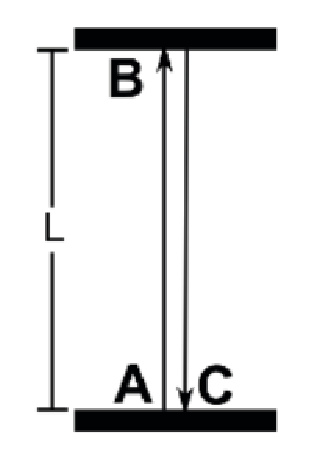
\includegraphics[scale=0.5]{fig2_1.eps}
    \figcaption{思想实验图示}
    \label{fig2.1}
}}
设想坐标系中一观察者,在原点处向上发出一个光脉冲,经过一段时间后被垂直镜面反射回原点。如图2.1所示

有3个重要的事件:
\begin{itemize}
  \item {\bf{A:}}光从原点发出
  \item {\bf{B:}}光在镜面上反射
  \item {\bf{C:}}光回到原点
\end{itemize}
事件{\bf{AC}}之间的时间间隔为\mpar{对于恒定速度$v$而言,有$v=\frac{\Delta s}{\Delta t}$,$\Delta s$表示经过的距离,$\Delta t$代表所需时间,因此$\Delta t=\frac{\Delta s}{v}$}
\begin{equation}\label{equ2.1}
\Delta t=t_C-t_A=\frac{2L}{c}
\end{equation}
式中$L$表示原点与反射点之间的距离。

{\marginpar{
        \centering
        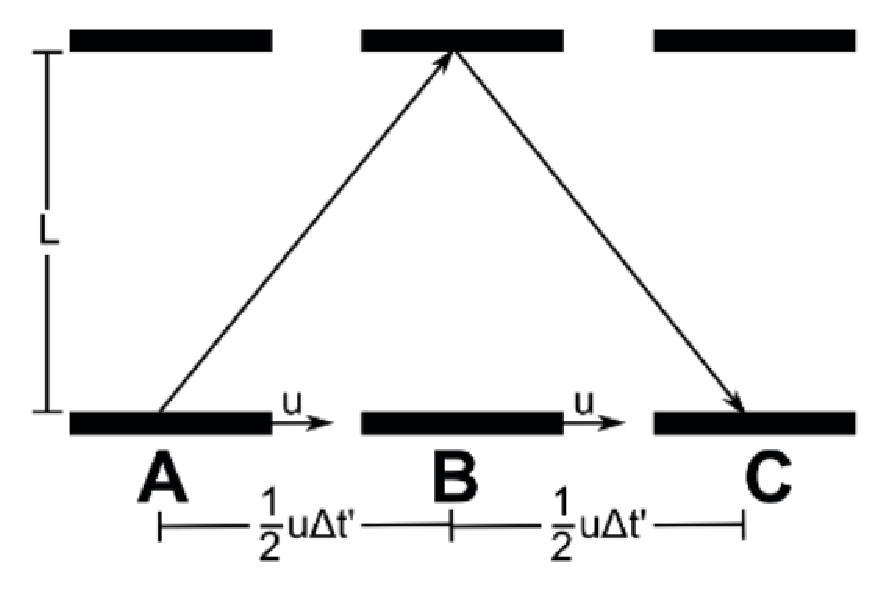
\includegraphics[scale=0.31]{fig2_2.eps}
        \figcaption{思想实验图示. 第二位移动观察者向左移动, 因此第一位观察者相对他向右移动}
        \label{fig2.2}
}}


接下来考虑第二位观察者,在$t_A$时刻处于他所在的坐标系的原点,并以恒定速度$u$相对于第一个观察者\mpar{那些能将两相对速度恒定的惯性参考系中的物理量相互转化的变换称为
{\bf{推动(Boost)}}变换, 后面我们会对此进行详述。}向左运动。为简便起见,我们假设第二个参考系的原点在$t_A$时刻与第一位观察者的坐标系原点重合。第二位观察者所见到的现象就与第一位不一样了。在他的参考系中,光脉冲的起点和终点并不在同一位置(见图2.2)。

用数学语言表示:
\begin{equation}\label{equ2.2}
  x'_A=0 \neq x'_C=u \Delta t' \qquad \rightarrow \qquad \Delta x' =u \Delta t'
\end{equation}
带撇物理量代表第二位观察者所测量的量。对于第一位静止系的观察者而言有
\begin{equation}\label{equ2.3}
  x_A=x_C \qquad \rightarrow \qquad \Delta x=0
\end{equation}
假定了第二位观察者运动沿$x$轴,因此
\begin{equation}\label{equ2.4}
 y'_A=y'_C \quad  \quad z'_A=z'_C \quad \rightarrow \quad \Delta y'=0 \quad  \quad \Delta z'=0
\end{equation}
那么同样也有
\begin{equation}\label{equ2.5}
 y_A=y_C \quad  \quad z_A=z_C \quad \rightarrow \quad \Delta y=0 \quad  \quad \Delta z=0
\end{equation}

接下来的问题是:{\bf{第二位观察者所测得的时间间隔是多少?}}因为已经假定了光速为常数,那么事件{\bf{AC}}对于第二位观察者而言将具有不同的间隔!时间间隔$\Delta t'=t'_C-t'_A$,等于光在第二位观察者的参考系中走过的距离$l$除以光速$c$。
\begin{equation}\label{equ2.6}
  \Delta t'=\frac{l}{c}
\end{equation}
我们可以利用古老的Pythagoras\footnote{通译为毕达哥拉斯。}定理(见图2.2) 计算光传播的距离
\begin{equation}\label{equ2.7}
  l=2 \sqrt{\left(\frac{1}{2} u \Delta t'\right)^2+L^2}
\end{equation}
利用式\eqref{equ2.6}可以得到
\begin{equation}\label{equ2.8}
  c \Delta t' =2 \sqrt{\left(\frac{1}{2} u \Delta t'\right)^2+L^2}
\end{equation}
再利用式\eqref{equ2.2}中的$\Delta x'=u\Delta t'$可得
\begin{displaymath}
c \Delta t' =
  2 \sqrt{\left(\frac{1}{2} u \Delta t'\right)^2+L^2}
\end{displaymath}
\begin{displaymath}
  \rightarrow
  \left( c \Delta t' \right)^2 =
   4 \left( \left(\frac{1}{2} u \Delta t'\right)^2+L^2 \right)
\end{displaymath}
\begin{equation}\label{equ2.9}
\rightarrow
\left( c \Delta t' \right)^2
-\left(\Delta x' \right)^2=
4 \left( \left(\frac{1}{2} u \Delta t'\right)^2+L^2 \right)
-\left(\Delta x' \right)^2 =4L^2
\end{equation}
 现在回到式\eqref{equ2.1},即$\Delta t =\frac{2L}{c}$,那么
\begin{equation}\label{equ2.10}
 \left( c \Delta t' \right)^2
 -\left(\Delta x' \right)^2
 =4 L^2
 =\left( c \Delta t \right)^2
 =\left( \Delta t c \right)^2
 -
 \!\!\!
 \underbrace{\left(\Delta x \right)^2}_{=0 \text{由式}2.3 \text{知}}
\end{equation}
终于,我们得到\mpar{\it{注意到我们在此处采用的是得到这个结果的最简方法,因为我们假定$t_A$时刻两坐标的原点是重合的。尽管如此,就算我们任意选择两惯性参考系原点的关系,仍然可以证明这个结论,只是过程会复杂一些。因为物理定律在任意惯性系中都是一样的,这给了我们任意选择便于计算的参考系的自由。如果第二位观察者的参考系运动方向是任意的,那就不再有$\Delta y'=0$和$\Delta z'=0$,但虽然如此,我们能够证明方程仍然是成立的,因为物理定律在任意惯性系中都是一样的。\footnote{译者注:原文的确把这句话说了两遍}}}

\begin{equation}\label{equ2.11}
\left( c \Delta t' \right)^2
-\left(\Delta x' \right)^2
-\underbrace{\left(\Delta y' \right)^2}_{=0}
-\underbrace{\left(\Delta z' \right)^2}_{=0}
=
\left( c \Delta t \right)^2
-\underbrace{\left(\Delta x \right)^2}_{=0}
-\underbrace{\left(\Delta y \right)^2}_{=0}
-\underbrace{\left(\Delta z \right)^2}_{=0}
\end{equation}
考虑第三个观察者,相对于第一个观察者以不同的速度运动,用同样的推理可以得到
\begin{equation}\label{equ2.12}
\left( c \Delta t'' \right)^2
-\left(\Delta x'' \right)^2
-\left(\Delta y'' \right)^2
-\left(\Delta z'' \right)^2
=
\left( c \Delta t \right)^2
-\left(\Delta x \right)^2
-\left(\Delta y \right)^2
-\left(\Delta z \right)^2
\end{equation}
因此,我们得到了一些对于所有观察者都相同的量:即二次式
\begin{equation}\label{equ2.13}
(\Delta s)^2
\equiv\left( c \Delta t \right)^2
-\left(\Delta x \right)^2
-\left(\Delta y \right)^2
-\left(\Delta z \right)^2
\end{equation}

此外,我们还能看出对于不同观察者,$(\Delta x)^2+(\Delta y)^2+(\Delta z)^2$或者说$(c\Delta t)^2$是不同的。我们将在下一节讨论不变量$\Delta s^2$所蕴含的物理意义。


\section[固有时]{Proper Time \quad 固有时}
\label{sec2.2}
我们在上一节推导出了狭义相对论中的不变量$\Delta s^2$,即在所有观察者眼中都相同的量。接下来我们要讨论这个量的物理意义。
    \marginpar{
        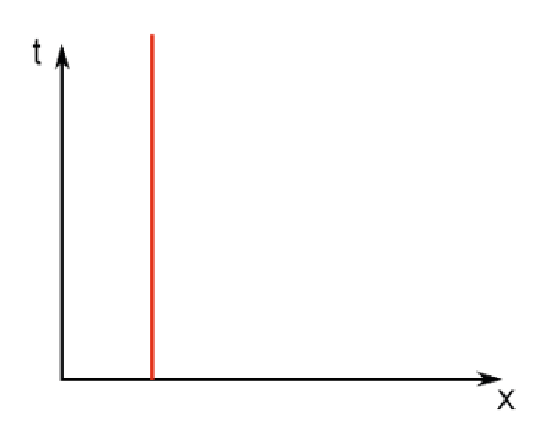
\includegraphics[scale=0.4]{fig2_3.eps}
        \figcaption{静止物体的世界线。物体位置不随时间流逝而变化。}
    }
为简便起见,我们将问题限制在一维空间中。对于一个相对于观察者静止的物体,我们能作出它的时空图(见图2.3)。相应的,一个匀速运动的物体能作出如图2.4所示的时空图。

    \marginpar{
        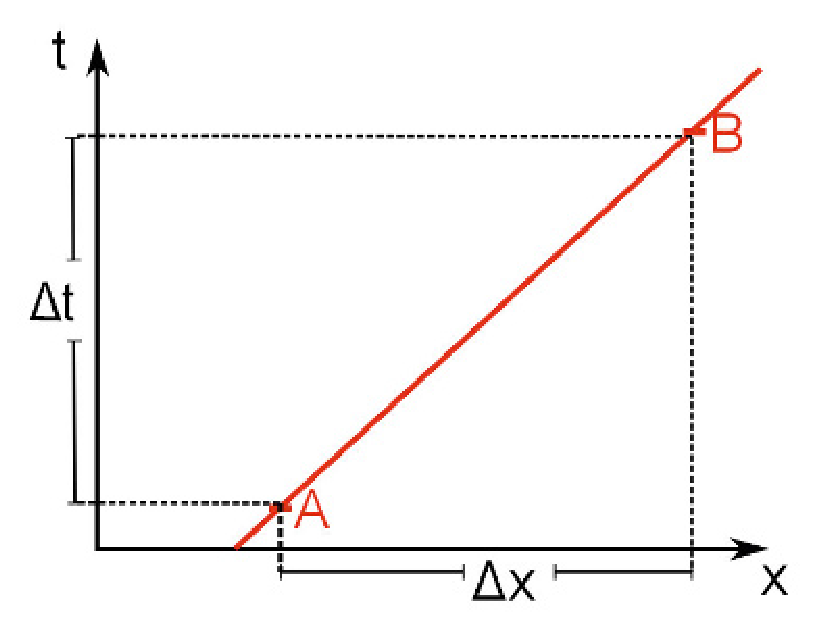
\includegraphics[scale=0.35]{fig2_4.eps}
        \figcaption{某匀速直线运动物体的世界线。物体前后经过某两点记为事件A,B。它们间的空间距离为$\Delta x$,时间间隔为$\Delta t$}
    }
我们画来用于确定物体在时空中位置的线称为{\bf{世界线(world line)}}。世界线总是依赖于观察者的。两不同观察者对于同一物体可能会画出完全不同的世界线。若一观察者眼中的物体时空图为图2.4,那么对于速度与物体相同的观察者,其时空图将为图2.5,即对于此观察者物体静止。为了解释两位观察者给出的不同描述,我们引入$x'$ 和$t'$ 表示第二位观察者的参考系中的时间和位置。

我们可以看到,两个观察者将对事件$AB$之间的变化持不同观点。对于第一位观察者,$\Delta x \neq 0$, 但对于第二位观察者,$\Delta x' = 0$。 两观察者都认为事件$A$ 和$B$ 之间的时间间隔非零:$\Delta t \neq 0$ 和$\Delta t' \neq 0$,且认为$\Delta s^2$也相同(见上节推导的结论,任意观察者都有相同的$\Delta s^2$)。 这将导出一个令人惊讶的结论:事件$A$ 到$B$ 经历的时间对于两观察者不同
    \marginpar{
        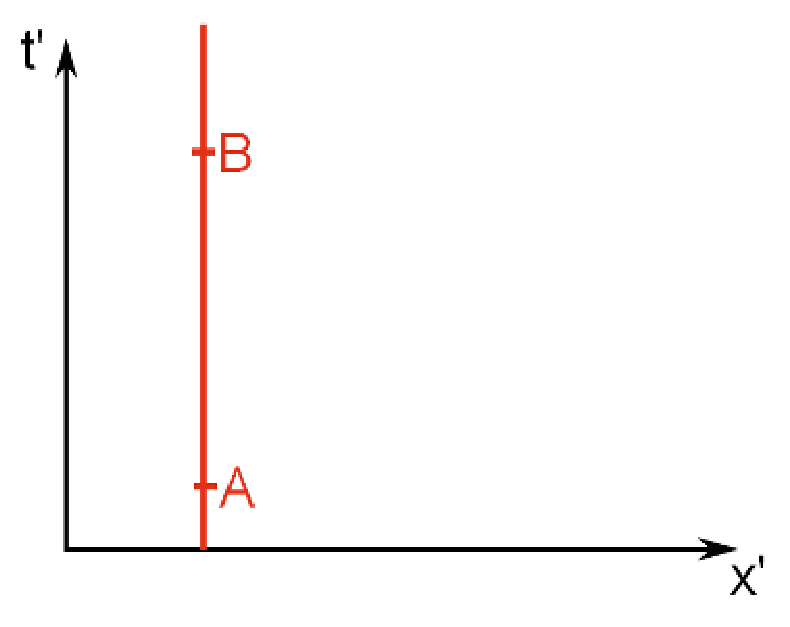
\includegraphics[scale=0.35]{fig2_5.eps}
        \figcaption{同一个运动物体的世界线,但观察者与该物体速度相同。该观察者观测到的事件AB之间的空间距离为$\Delta x' = 0$}
    }
\begin{equation}\label{equ2.14}
  (\Delta s)^2
  =(c\Delta t)^2
  -(\Delta x)^2
\end{equation}
\begin{equation}\label{equ2.15}
  (\Delta s')^2
  =(c\Delta t')^2
  -\underbrace{(\Delta x')^2}_{=0}
  =(c\Delta t')^2
\end{equation}
\begin{equation}\label{equ2.16}
   (\Delta s)^2
   = (\Delta s')^2
   \rightarrow
    (\Delta t')^2 \neq
     (\Delta t')^2
     \quad \text{因为}  (\Delta x)^2 \neq 0
\end{equation}

这是有关狭义相对论最著名的一个效应,通常称为{\bf{钟慢效应(time-dilation)}}。时间间隔依赖于观察者,正如空间距离一样。不同观察者时间流逝速度不同,因此两事件经历的时间也就自然不同了。

现在时间将变为一个相对的概念,如果我们能找到一个对于所有观察者都相同的时间量,这将会非常有用。在上述例子中,第二位观察者与物体有相同的速度,有
\begin{equation}\label{equ2.17}
  (\Delta s')^2
  =(c\Delta t')^2
\end{equation}

上式意味着狭义相对论中的不变量恰为观察者所观测到的时间间隔乘上光速$c$。这让我们有机会能用$(\Delta s)^2$定义一个对于所有观察者相同的时间量。我们定义
\begin{equation}\label{equ2.18}
  (\Delta s)^2
  =(c\Delta \tau)^2
\end{equation}
$\tau$称为{\bf{固有时(proper time)}}。固有时是所有相对于该物体静止的观察者所测量的时间。

当然,现实生活中的物体绝非只能做匀速运动,但我们可以取足够短的时间(无穷小),使得运动近似为匀速运动,这样固有时的概念就说得通了。因此数学上我们需将概念过渡到无穷小,即$\Delta \rightarrow d$:
\begin{equation}\label{equ2.19}
  (ds)^2  =(cd \tau )^2=(cdt)^2-(dx)^2-(dy)^2-(dz)^2
\end{equation}

因此,就算一个物体到处乱跑,我们也能假设一个与物体一起运动的自带时钟的观察者,这样他总与该物体相对静止。对于这个特定的观察者而言,他所测量的时间间隔就是固有时,这一数值对其余观察者也是相同的,因为$(ds)^2=(cd\tau)^2$对于任意观察者成立。再次强调,这并不意味着对所有观察者都有同样的时间间隔,只是这些观察者承认该特殊观察者所测量的时间间隔为一不变量罢了。

\section[速度上限]{Upper Speed Limit \quad 速度上限}
\label{sec2.3}
在上节中我们对狭义相对论这一不变量有了解释,现在可以更进一步,导出另一个狭义相对论的惊人结论。

由于不变量的定义中带有负号,这意味着对于时空中的两个事件,$(\Delta s)^2$的值可能为0。$(\Delta s)^2$的值甚至可能是负的,但这样我们将得到一个复的固有时\mpar{按固有时定义,$(ds)^2=(cd\tau)^2$,$(ds)^2 < 0 \rightarrow d\tau$ 为复数。},通常复的固有时没有物理意义。因此,$(\Delta s)^2=0$时固有时最小,$\tau=0$,令
\[
\Delta s^2_{min}
=0=(c \Delta t)^2-(\Delta x)^2-(\Delta y)^2-(\Delta z)^2
\]
\[
\rightarrow (c \Delta t)^2
=(\Delta x)^2+(\Delta y)^2+(\Delta z)^2
\]
\begin{equation}\label{equ2.20}
 \rightarrow c^2=
  \frac{(\Delta x)^2+(\Delta y)^2+(\Delta z)^2}{(\Delta t)^2}
\end{equation}
在上式右侧我们有速度平方$v^2$,也就是距离除上时间,把这个式子写成极限,则
\begin{equation}\label{equ2.21}
 \rightarrow c^2=\frac{(d x)^2+(d y)^2+(d z)^2}{(dt)^2}
\end{equation}
函数$x(t)$,$y(t)$,$z(t)$是描述两事件之间路径的参数方程,这样式子右侧就是两事件间的运动速率。
%flag 此处的速度在文中并无主语,可能要加上物体二字,那么前面也得改。

因此,当某一观察者测得的固有时为$0$时其速度将满足下式
\begin{equation}\label{equ2.22}
  \rightarrow c^2 =v^2
\end{equation}
这意味着没有物体能以超过光速$c$的速度运动!\footnote{译者注:否则其固有时为复}{\bf{我们给物理学中的一切事物找到了一个速度上限。}}时空中的两事件的联系不能超光速。

{\it{这一点满足物理学上的{\bf{局域性原理(principle of locality)}},即物理学中的对象只能被它邻近的对象影响。相互作用都是局域的,不存在超距作用,物理效应的传播需要时间。}}

\section[Minkowski记法]{The Minkowski Notation \quad Minkowski 记法}
\label{sec2.4}
\begin{quote}
从现在起,孤立的空间和孤立的时间注定要消失成为影子,只有两者的统一才能保持独立的存在。
\end{quote}
\begin{flushright}
  {\bf{-Hermann Minkowski}}\mpar{出自Hermann Minkowski在Assembly of German Natural Scientists and Physicians(1908.9.21)上的演讲}
\end{flushright}
写出狭义相对论中不变量
\begin{equation}\label{equ2.23}
 ds^2=(cdt)^2-(dx)^2-(dy)^2-(dz)^2
\end{equation}
在此处将采用一种新的记法,这种记法初学时可能稍显复杂,不过后文中将经常用到:\\
\begin{align}
ds^2&=\eta^{\mu\nu}dx_\mu dx_\nu \notag \\
&=\eta^{00}(dx_0)^2+\eta^{11}(dx_1)^2+\eta^{22}(dx_2)^2+\eta^{33}(dx_3)^2 \notag \\
&=dx_0^2-dx_1^2-dx_2^2-dx_3^2\notag \\
&=(cdt)^2-(dx)^2-(dy)^2-(dz)^2 \label{equ2.24}
\end{align}
在这里我们用了一些新的约定和记号,这些东西在近代物理中应用很广泛,所以越早熟悉越好:
\begin{itemize}
  \item Einstein求和约定:某指标在同一项内出现两次则代表遍历该指标并求和。例如:$\sum_{i=1}^3a_i b_i =a_i b_i=a_1 b_1 +a_2 b_2 +a_3 b_3$,但$\sum_{i=1}^3a_i b_j=a_1 b_j +a_2 b_j +a_3 b_j\neq a_i b_j$
  \item 像$\mu$,$\nu$,$\sigma$这样的希腊字母
  \mpar{像 $i$,$j$,$k$这样的罗马字母作指标时一般代表从1到3求和:$x_i x_i \equiv \sum_i^3 x_i x_i$。 后面我们还会用到大写的罗马字母如$A$,$B$,$C$,它们作指标时代表从1到8求和。} 作指标时,一般代表从0 到3 求和:$x_\mu y_\mu=\sum_{\mu=0}^3 x_\mu y_\mu $
  \item 我们约定变量$x_0\equiv ct$,$x_1\equiv x$,$x_2\equiv y$,$x_3\equiv z$。这样时间空间地位等同,也便于我们使用Einstein求和约定
  \item 引入Minkowski度规($\eta$看作一矩阵,$\eta^{ij}$ 为其矩阵元):$\eta^{00}=1$,$\eta^{11}=-1$,$\eta^{22}=-1$,$\eta^{33}=-1$,当$\mu \neq \nu$时$\eta^{\mu\nu}=0$  (也可以等价的写为
\mpar{$\eta^{\mu\nu}= \\ \\
       \left(
       \begin{array}{cccc}
        1 & 0 & 0 & 0 \\
         0 & -1 & 0 & 0 \\
          0 & 0 & -1 & 0 \\
          0 & 0 & 0  & -1\\
        \end{array}
        \right)$ }
      $\eta^{\mu\nu} = \mathrm{diag} (1,-1,-1,-1)$)
\end{itemize}

另外按常规我们还要引入{\bf{四维矢量(four-vector)}},简称{\bf{4矢}}。
\begin{equation}\label{equ2.25}
  dx_\mu =\left(\begin{array}{c}
            dx_0 \\
            dx_1 \\
            dx_2 \\
            dx_3
          \end{array}\right)
\end{equation}
式\eqref{equ2.24}可用4矢和Minkowski度规表出
\begin{align}
  &(ds)^2=dx_\mu \eta^{\mu\nu} dx_\nu \notag \\
  &=\left(
     \begin{array}{cccc}
       dx_0 & dx_1 & dx_2 & dx_3 \\
     \end{array}
   \right)
   \!\!\!
   \left(
     \begin{array}{cccc}
       1 & 0 & 0 & 0 \\
       0 & -1 & 0 & 0 \\
        0 & 0 & -1 & 0 \\
        0 & 0 & 0  & -1\\
     \end{array}
   \right)
   \!\!\!
   \left(
     \begin{array}{c}
       dx_0 \\
        dx_1 \\
       dx_2 \\
        dx_3\\
     \end{array}
   \right)\notag \\
   &=dx_0^2-dx_1^2-dx_2^2-dx_3^2 \label{equ2.26}
\end{align}

采用这种记法能让我们省不少事。对于$ds$,我们给出的解释是时空(Minkowski时空)中两事件的“距离”,这个“距离”并不只是空间距离,它还将时间间隔考虑在内。如果我们考虑3维Euclidean 空间\mpar{3维Euclidean空间就是经典物理中一般的空间,在此空间中我们将时间和空间分别处理,也就是未将时空考虑成一个整体的几何结构来考虑。但一旦将时间作为新坐标,结合出时空的观念,我们便能将时间空间放在同一坐标下考虑。}中两点间最短距离的平方\mpar{Kronecker函数$\delta_{ij}$即是单位矩阵在指标记法下的表示,详见附录\ref{appendix.B.5.5}}
\begin{align}
  (ds)^2&=dx_i \delta^{ij} dx_j \notag \\
            &=\left(
               \begin{array}{ccc}
                dx_1 & dx_2 & dx_3 \\
               \end{array}
               \right)
               \left(
               \begin{array}{ccc}
                1 & 0 & 0  \\
                0 & 1 & 0  \\
                0 & 0 & 1  \\
              \end{array}
              \right)
              \left(
              \begin{array}{c}
               dx_1 \\
               dx_2 \\
               dx_3\\
              \end{array}
              \right)\notag \\
           &=(ds)^2=(dx_1)^2+(dx_2)^2+(dx_3)^2\label{equ2.27}
\end{align}

这种能够告诉我们无限临近的两点间的距离叫{\bf{度规(metric)}}。在Euclidean空间中度规就是单位矩阵$\delta_{ij}$。在广义相对论的弯曲时空中将会有更复杂的度规,但在狭义相对论中我们采用的是相对简单的Minkowski度规$\eta^{\mu\nu}$。度规是计算长度的工具,我们可以通过度规定义{\bf{4矢的长度(length of a four-vector)}},即4矢与自身的标量积\mpar{此定义在Euclidean空间中同样适用:由于度规为
$\delta_{ij}=\left(
 \begin{array}{ccc}
 1 & 0 & 0  \\
  0 & 1 & 0  \\
  0 & 0 & 1  \\
  \end{array}
  \right)
$,易得矢量$\vec{v}$的长度$=\vec{v}\cdot\vec{v}=v_1^2+v_2^2+v_3^2$。}
\[
x^2=x \cdot x \equiv x_\mu x_\nu \eta^{\mu\nu}
\]
类似地,两任意4矢的标量积定义为
\begin{equation}\label{equ2.28}
  x\cdot y\equiv x_\mu y_\nu \eta^{\mu\nu}
\end{equation}

对于上下标,也有一些约定能使计算过程更清晰。我们定义带有 上指标的4矢\mpar{带有下指标的4矢通常叫做协变4矢,带有上指标的4 矢通常叫做逆变4矢。}
\begin{equation}\label{equ2.29}
  x^{\mu}\equiv\eta^{\mu\nu}x_\nu
\end{equation}
或者
\begin{equation}\label{equ2.30}
  y^{\nu}\equiv\eta^{\mu\nu}y_\mu
 \!\!\!\!\!\!\!\!\!\!\!\!\!\!\!\!\!\!\!\!\!\!\!\!\!\!\!\!
 \underbrace{=}_{Minkowski\text{度规是对称的}\eta^{\mu\nu}=\eta^{\nu\mu}}
 \!\!\!\!\!\!\!\!\!\!\!\!\!\!\!\!\!\!\!\!\!\!\!\!\!\!\!\!
  \eta^{\nu\mu}y_\mu
\end{equation}
因此,标量积可以写为\mpar{指标的名称如何选取并不影响最后的值,详见附录\ref{appendix.B.5.1}。}
\begin{equation}\label{equ2.31}
  x\cdot y\equiv x_\mu y_\nu \eta^{\mu\nu}=x_\mu y^\mu=x^\nu y_\nu
\end{equation}
上式中,变换的上指标是可以任意选择的,这只是为了避免公式中总是出现$\eta^{\mu\nu}$的一种方法,正如引入Einstein求和约定是为了避免总是出现求和号一样。

\section[Lorentz变换]{Lorentz Transformations \quad Lorentz变换}
\label{sec2.5}
下一步,我们将尝试找出两参考系之间不违背狭义相对论基本假设的变换方式。由上文可知,从狭义相对论的两个基本假设可以推出对于所有惯性参考系均有$ds^2=\eta^{\mu\nu} dx_\mu dx_\nu $,即
\begin{equation}\label{equ2.32}
  ds'^2= dx'_\mu dx'_\nu \eta^{\mu\nu}
  =ds^2
  =dx_\mu dx_\nu\eta^{\mu\nu}
\end{equation}
因此,两参考系间所允许的变换要能保证这个二次式的形式和Minkowski时空中的标量积在变换下不变。设变换为$\Lambda$,那么变换后
\begin{equation}\label{equ2.33}
  dx_\mu \rightarrow dx'_\mu=\Lambda^\sigma_\mu dx_\sigma
\end{equation}
由于$(ds)^2$在变换下不变
\begin{align}
(ds)^2&=(ds')^2 \notag\\
\rightarrow dx\cdot dx &\overset{\text{!}}{=} dx' \cdot dx' \notag \\
\rightarrow dx_\mu dx_\nu\eta^{\mu\nu} &\overset{\text{!}}{=} dx'_\mu dx'_\nu\eta^{\mu\nu} \underbrace{=}_{\mathclap{\eqref{equ2.33}\text{式}}} \Lambda_\mu^\sigma dx_\sigma \Lambda_\nu^\gamma dx_\gamma\eta^{\mu\nu}\notag \\
\underbrace{\rightarrow}_{\mathclap{\text{重命名哑指标}}} dx_\mu dx_\nu\eta^{\mu\nu} &\overset{\text{!}}{=} \Lambda^\mu_\sigma dx_\mu \Lambda^\nu_\gamma dx_\nu\eta^{\sigma\gamma}\notag\\
\underbrace{\rightarrow}_{\mathclap{因为dx_\nu\text{任意}}} \eta^{\mu\nu} &\overset{\text{!}}{=} \Lambda^\mu_\sigma\Lambda^\nu_\gamma\eta^{\sigma\gamma}\label{equ2.34}
\end{align}
或者用矩阵形式来写\mpar{详见附录\ref{appendix.C.1}。}
\begin{equation}\label{equ2.35}
  \eta=\Lambda^{\mathrm{T}}\eta\Lambda
\end{equation}

{\bf{此即变换$\Lambda_\mu^\nu$所需满足条件。}}

这个条件现在看起来可能有些奇怪,但在后文中我们会用更自然的方式导出这个条件。在下一章里,我们会看到Euclidean空间中的旋转所导出的变换%
\mpar{稍后会讲明$O$的意义。}$O$能够保证Euclidean 空间的标量积不变\mpar{“$\cdot$”表示的是矢量的点乘,如果我们将矢量写为列向量,那么按矩阵相乘的定义有$\vec{a}\cdot\vec{b}=\vec{a}^\mathrm{T}\cdot\vec{b}$。 有关$(Oa)^\mathrm{T}=a^\mathrm{T}O^\mathrm{T}$这一点详见附录\ref{appendix.C.1},式\ref{equC.3}。}% 此处原文有误
\begin{equation}\label{equ2.36}
  \vec{a} \cdot \vec{b}
  \overset{\text{!}}{=}
  \vec{a'} \cdot \vec{b'}
  \!\!\!\!\!\!\!\!\!\!
  \underbrace{=}_{\text{注意}
  (Oa)^\mathrm{T}=a^\mathrm{T}O^\mathrm{T}}
  \!\!\!\!\!\!\!\!\!\!
  \vec{a}^\mathrm{T} O^\mathrm{T} O\vec{b}
\end{equation}
因此
\mpar{这一条件一般称为{\bf{正交性(orthogonality)}}条件,因此用字母$O$表示。满足$O^\mathrm{T} O={\bf{1}}$的矩阵称为正交矩阵,因为它列与列之间是正交的。换句话说,矩阵的每一列都可以看做一个矢量,正交性条件就是说这些矢量相互正交。}

$O^\mathrm{T} {\bf{1}} O\overset{\text{!}}{=}{\bf{1}}$,恰巧Euclidean 空间的度规就是单位矩阵${\bf{1}}$,其地位正如Minkowski 度规在式\eqref{equ2.35} 中一样。这个性质是旋转的定义中的一部分,旋转不能改变矢量的长度,即在数学上保证标量积不变
\mpar{矢量的长度即是矢量与自身的标量积的平方根。}\footnote{译者注:$\vec{a}\cdot \vec{b}=\frac{1}{2} [(\vec{a}+\vec{b})^2-\vec{a}^2-\vec{b}^2]$,若保证模长不变,标量积也不变。}此外我们还注意到旋转不改变坐标系的方向\mpar{详见附录\ref{appendix.A.5}。},这表明 $\text{det}(O) \overset{\text{!}}{=}1$,因为保证标量积不变的变换除了旋转变换还有空间反演\mpar{空间反演可简单地理解为映射$\vec{x}\rightarrow -\vec{x}$。这种变换满足$\text{det}(O) \overset{\text{!}}{=}$及$O^{\mathrm{T}}O={\bf{1}}$。 因此,如果我们要将变换限制为旋转变换,就需要加上条件$\text{det} (O) \overset{\text{!}}{=} {\bf{1}}$。此外,空间反演变换又称宇称变换。}。

我们定义保Minkowski时空中标量积不变的变换为
{\bf{Lorentz变换(Lorentz transformations)}}
,这也是为保证狭义相对论的假设所必需的。相应的,每当我们需要得到在Lorentz变换下不变的项时,{\it{都必须结合上下指标}}:$x_\mu y^\mu=x_\mu y_\nu \eta^{\mu\nu}$。
在我们学会了一些非常优雅的技术来处理这样的情况之后,我们会在下一章构建这些转换具体的矩阵形式。
\section[不变性,对称性,协变性]{Invariance, Symmetry and Covariance 不变性,对称性,协变性}
在我们继续之前,有一些重要的概念要事先声明。首先,一个量要称为{\bf{不变量(invariant)}},这个量必须在变换下不变。比如说,我们考虑一个依赖于不同的量$A,B,C,\dots$任意函数$ F$,$F=F(A,B,C,\dots)$,如果我们将$A,B,C,\dots$变换为$A',B',C',\dots$,有
\begin{equation}\label{equ2.37}
  F(A',B',C',\dots)=F(A,B,C,\dots)
\end{equation}
那么$F$称为变换下的一个不变量。我们可以用对称性来描述。
{\bf{对称性(symmetry)}}是指在某一变换下或者某一系列变换下保持不变的性质。举个例子,如果说一个物理系统在任意的旋转变换下不变,那么该系统具有旋转对称性。再比如说,一间室温为常温的房间,房间内各点的温度与位置无关,换言之,如果把所有的点朝着某特定方向平移一段距离,室温不变。因此我们说室温具有{\it{平移对称性}}。

协变性与不变性有共通之处而又不同。如果一个方程在变换下形式不变,那么称这个方程具有协变性。例如下面这个式子
\[
E_1=a A^2+bBA'+cC^4
\]
在变换之后这个方程写为
\[
E'_1=a A'^2+bB'A'+cC'^4
\]
那么这个方程具有协变性,因其在变换下形式不变。另一方程
\[
E_2=x^2+4axy+z
\]
若在变换之后写为
\[
E'_2=y'^3+4az'y'+y'^2+8z'x'
\]
那么它就不是协变的,因为其形式已经变化。

所有的物理规律都应具有Lorentz协变性\footnote{即在Lorentz变换下具有协变性---译者(InSight)},因为只有这样的物理规律才能在任意参考系下成立。非协变的物理规律只能在某一特定参考系下成立,这会导致在东京和纽约具有不同的物理规律。显然这个主意糟透了,因为不存在一个特殊的参考系,我们得让物理规律在任意参考系中成立。我们将在后文中学到如何用协变的方法计算物理规律。

\section*{Further Reading Tips\quad 阅读建议}
\begin{itemize}
\item {\bf E.Taylor and J.Wheeler - Spacetime Physics:Introduction to Special Relativity}\mpar{Edwin F.Taylor and John Archibald Wheeler.\\ {\it Spacetime Physics}.\\W.H.Freeman,2nd edition,\\3 1992.ISBN 9780716723271}适合用来入门。
\item {\bf D.Fleisch - A Student’s Guide to Vectors and Tensors}\mpar{Daniel Fleisch.\\{\it A Student’s Guide \\ to Vectors and Tensors}.\\ Cambridge
University Press,\\1st edition,11 2011.ISBN 9780521171908}对狭义相对论中用到的张量范式有很有创意的解释。比如对于协变与逆变分量的差异。
\item {\bf N.Jeevanjee - An Introduction to Tensors and Group Theory for Physicists}\mpar{Nadir Jeevanjee. \\{\it An Introduction to Tensors and Group Theory for Physicists}.\\Birkhaeuser,1st edition,August 2011.\\ISBN 978-0817647148}是另一本把在狭义相对论中用到的数学讲的不错的书。
\item {\bf A.Zee - Einstein Gravity in a nutshell}\mpar{Anthony Zee.\\{\it Einstein Gravity in a
Nutshell}.\\Princeton University Press,\\1st
edition,5 2013.\\ISBN 9780691145587}是一本关于广义相对论的书,但是里面也有很多关于狭义相对论的很棒的解释。
\end{itemize}

%!TEX encoding = UTF-8 Unicode

\part{Symmetry Tools 对称性工具}

%!TEX encoding = UTF-8 Unicode

%----------------------------------------------------------------------------------------
%	CHAPTER 3
%	Translator: SI(= Surgam Identidem)
%----------------------------------------------------------------------------------------

\chapterimage{chapter_head_1.pdf} % Chapter heading image

\makeatletter 
\newcommand\figcaption{\def\@captype{figure}\caption} 
\newcommand\tabcaption{\def\@captype{table}\caption} 
\makeatother




\chapter[Lie群]{Lie Group Theory\quad  Lie群}
\label{chap3}

\section*{本章概述}



\marginpar{\tiny
	
下面的图表是本章结构的示意图. 当你迷失方向的时候记得回来看看, 初学的时候不太需要看它.\sout{反正也看不懂}

\setlength{\unitlength}{0.8cm}
\begin{picture}(4, 3)\thicklines
\put(1.5, 1.8){\makebox(2.5, 1.2){\text{二维旋转}}}
\put(1, 0.7){\vector(1, 1){1.4}}
\put(4, 0.7){\vector(-1, 1){1.4}}
\put(0.5, 0.2){\makebox{$\mathcal{U}(1)$}}
\put(4, 0.2){\makebox{$\mathcal{SO}(2)$}}
\put(0, 0){\line(5, 0){5.5}}
\end{picture}

\begin{picture}(4, 3)\thicklines
\put(1.5, 1.8){\makebox(2.5, 1.2){\text{三维旋转}}}
\put(1, 0.7){\vector(1, 1){1.4}}
\put(4, 0.7){\vector(-1, 1){1.4}}
\put(0.5, 0.2){\makebox{$\mathcal{SU}(2)$}}
\put(4, 0.2){\makebox{$\mathcal{SO}(3)$}}
\put(0, 0){\line(5, 0){5.5}}
\end{picture}

\begin{picture}(5, 5)\thicklines
\put(1.5, 4){\makebox(2.5, 1.2){\text{Lorentz变换}}}
\put(2.5, 4.3){\vector(0, -1){0.8}}
\put(1.5, 2.5){\makebox(2.5, 1.2){ \text{Lie代数} $\hat{=} \, \mathfrak{su}(2) \oplus \mathfrak{su}(2) $  }}
\put(2.5, 2.8){\vector(0, -1){0.8}}
\put(1.5, 1){\makebox(2.5, 1.2){\text{双覆盖表示}}}
\put(0, 1){\line(5, 0){5.5}}
\end{picture}

\begin{picture}(5, 3)\thicklines
\put(1.5, 3){\makebox(2.5, 1.2){\text{Lorentz变换 + 平移}}}
\put(2.5, 3.2){\vector(0, -1){0.8}}
\put(1.5, 1.6){\makebox(2.5, 1.2){ \text{Poincare群} }}
\end{picture}

}

本章的最终目的是导出{\bf{Poincare群双覆盖的基本表示}}, 物理学现在认为Poincare群是时空根本的对称性群. 这些基本表示是描述所有基本粒子的必要工具, 每一种表示对应一种基本粒子, 它们揭示了自然界存在何种基本粒子.

我们从两个简单例子引出{\bf{群}}的定义, 然后作为学习Lie群理论的第一步, 我们讨论描述二维旋转变换的两种方式:
\begin{itemize}
	\item $2 \times 2$旋转矩阵.
	\item 单位复数.
\end{itemize}

接着我们尝试找出描述三维旋转的第二种方法(像复数那样, 当然第一种方法是$3\times3$矩阵), 第二法与一种超级重要的群 --- {\bf{$SU(2)$}}.\mpar{$S$表示特殊(special), 它的含义为$\det (M) = 1$. U表示幺正: $M^\dagger M = 1$, 数字$2$表示这个群起初是用$2 \times 2$矩阵定义的.}有关. 之后我们研究{\bf{Lie代数}}, 使用简便的Lie代数能够深入研究复杂的Lie群. 不同的群可以有相同的Lie代数, 但只有其中的一部分是基本的. 
从上述基础出发就能准确揭示自然的基本对称性群 --- Poincare群的双覆盖. 
%flag1:  double covers the Poincare group. (Poincare 群的双覆盖) 翻译是否正确?
我们将利用已知的变换操作导出Lie代数, 并利用Lie代数得出不同的对称变换表示. 这样就能看出我们开始时使用的表示其实只是一种特殊情况. 这样我们又能研究Poincare群的重要部分 --- {\bf{Lorentz群}}, 我们会看到Lorentz群双覆盖的Lie代数由两份$SU(2)$\,Lie代数所组成, 因此我们可以直接利用熟悉的$SU(2)$群的结论. 最后我们将平移变换考虑进来, 这就是Poincare群, Poincare群就是Lorentz群加上平移. 完成上述所有之后我们终于可以将Poincare群双覆盖的基本表示进行分类, 这些在后面的章节中会大用特用, 我们将从中导出物理学的基本定律.

\section[群]{Groups\quad 群}
\label{sec3.1}
我们需要合适的数学工具描述对称性\sout{以和民科(贬义的)区分开}. 描述对称的数学分支称为{\bf{群论}}. 群论的一个分支{\bf{Lie理论}}\sout{谎言理论}描述连续的对称性, 物理中经常遇到这种情况.

我们把对称性定义为变换下的不变性, 而描述对称的群就定义为某些变换的集合. 让我们从两个简单例子开始体会群到底该怎么定义吧.



\begin{enumerate}
	\item 正方形是一些点的集合(例如四个顶点是该集合的一部分), 正方形的对称性是在某些变换下(变换: 将一个点映射到另一个点)保持不变的性质.
		
	符合条件的变换有绕中心旋转$90^\circ, 180^\circ, 270^\circ, 0^\circ$等等. 这些旋转操作将正方形映射到它自身. 我们称这个集合(正方形点集)在这样的变换下具有不变性.
	% flag1: This means they map every point of the set to a point that lies again in the set 没翻译, 因为觉得太啰嗦...
	
	\marginpar{
		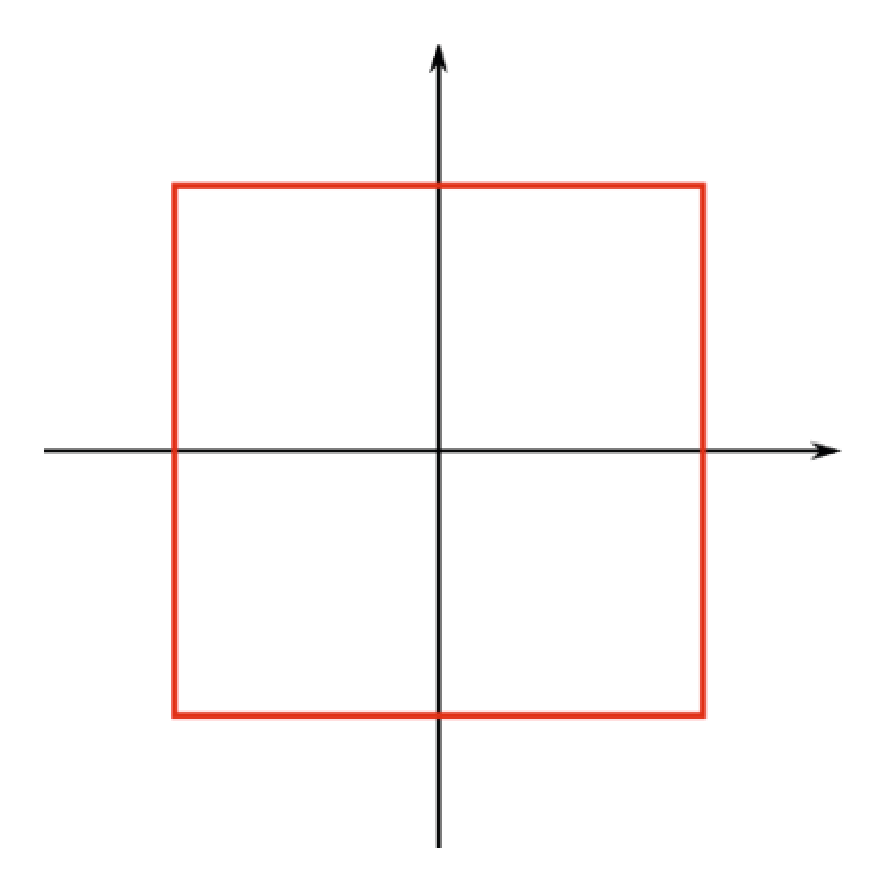
\includegraphics[scale=0.35]{fig3_1} 
		\figcaption{正方形}
	}
	
	\marginpar{
		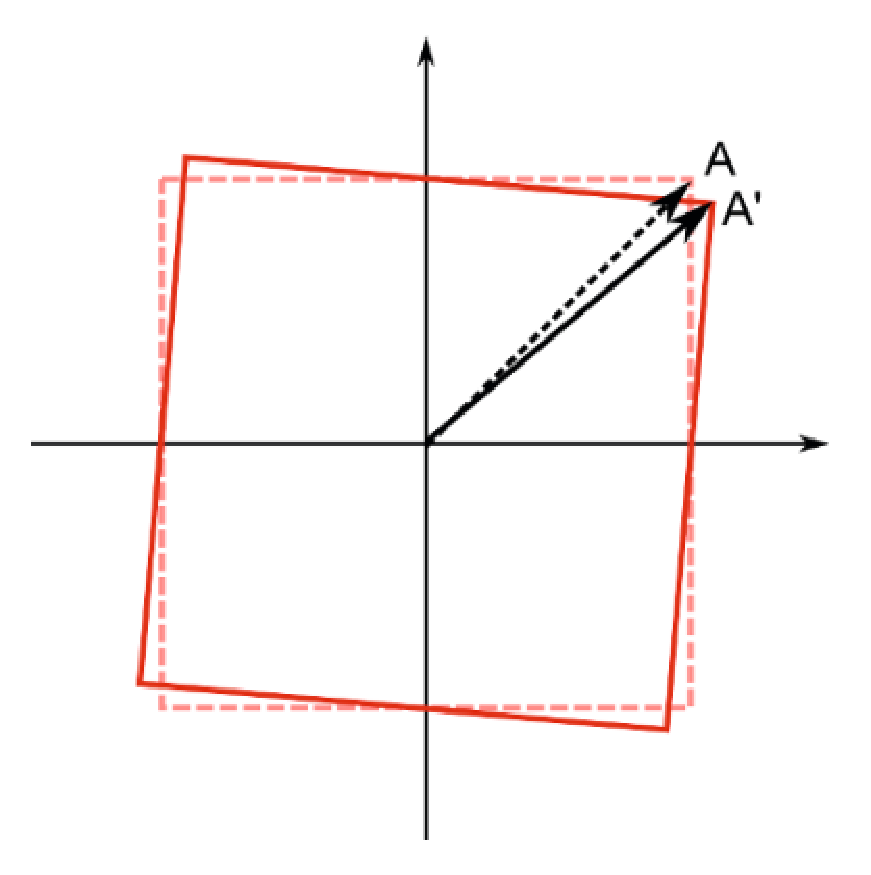
\includegraphics[scale=0.35]{fig3_2.eps}
		\figcaption{正方形绕中心顺时针旋转$5^\circ$}
	}
	
	注意不是所有旋转变换都对称. 我们关注顶点的变化就能看出来, 比如绕中心顺时针旋转$5^\circ$, 这个变换将顶点映射到原来正方形点集之外, 顶点$A$映射到了原来正方形集合之外的点$A'$. 因此这个旋转变换对正方形不具有对称性. 当然, 变换后的点集仍然是个正方形, 但却是不同的正方形(即不同点的集合). 绕中心转$90^\circ$是对称的, 如图\ref{fig3.3}, 顶点$A$变换到点$B$, 等等, 原来的正方形点集变换到相同的集合.
	
	{
	\centering{
	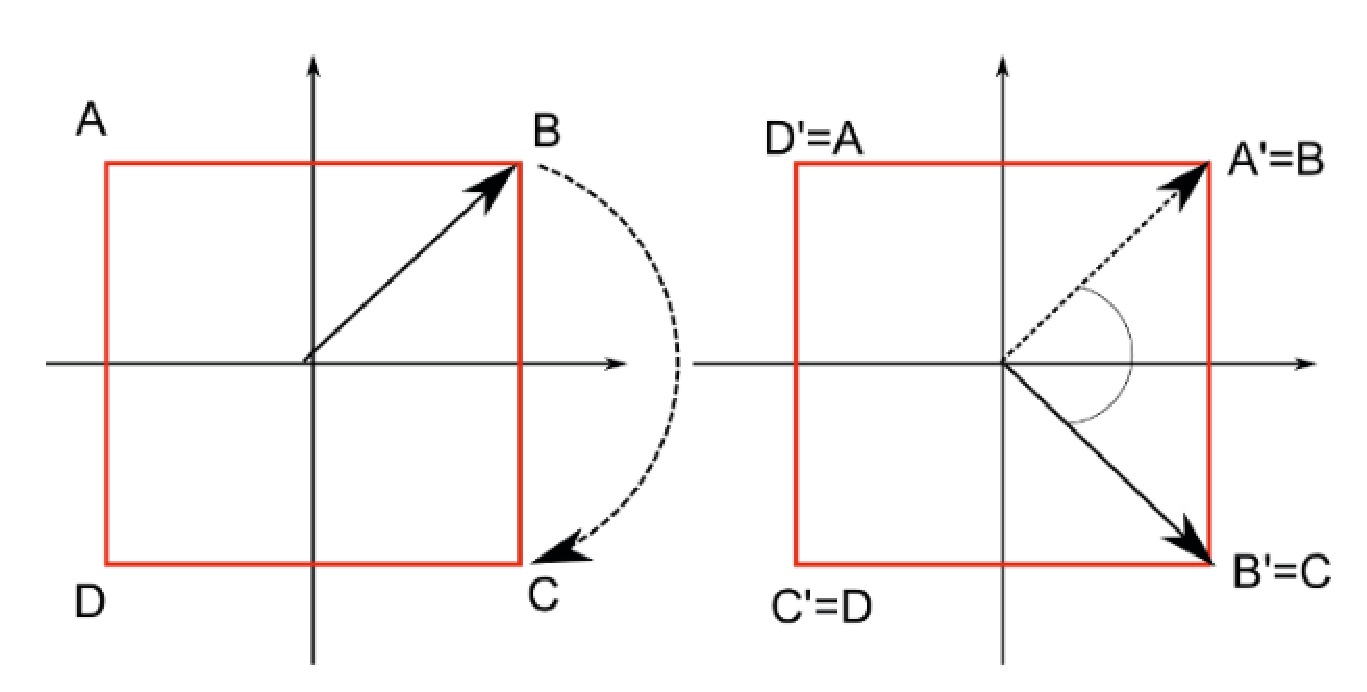
\includegraphics[scale=0.4]{fig3_3}
	\figcaption{正方形绕中心旋转$90^\circ$}
	\label{fig3.3}
	}}
	
	假如你看了一眼原来的正方形, 然后闭上眼睛, 这时有人把正方形做了一个变换. 如果你不能分辨这个正方形是否发生变化, 那么这个变换就是个对称变换.
	
	我们把所有使正方形不变的变换构成的集合称为群. 变换参数(本例中就是旋转角度)不能任意取值(而是取分立的数), 这个群称为离散群.
	
	\item 另一个例子是使单位圆不变的变换构成的集合. 类似地, 单位圆还是一些点构成的集合, 对称变换把这个集合映射到它自身.
	
	单位圆绕圆心旋转任意角度都不变. 换言之, 变换参数(这里就是旋转角度)可以取任意值, 因此这个群称为连续群.
\end{enumerate}
	\marginpar{
		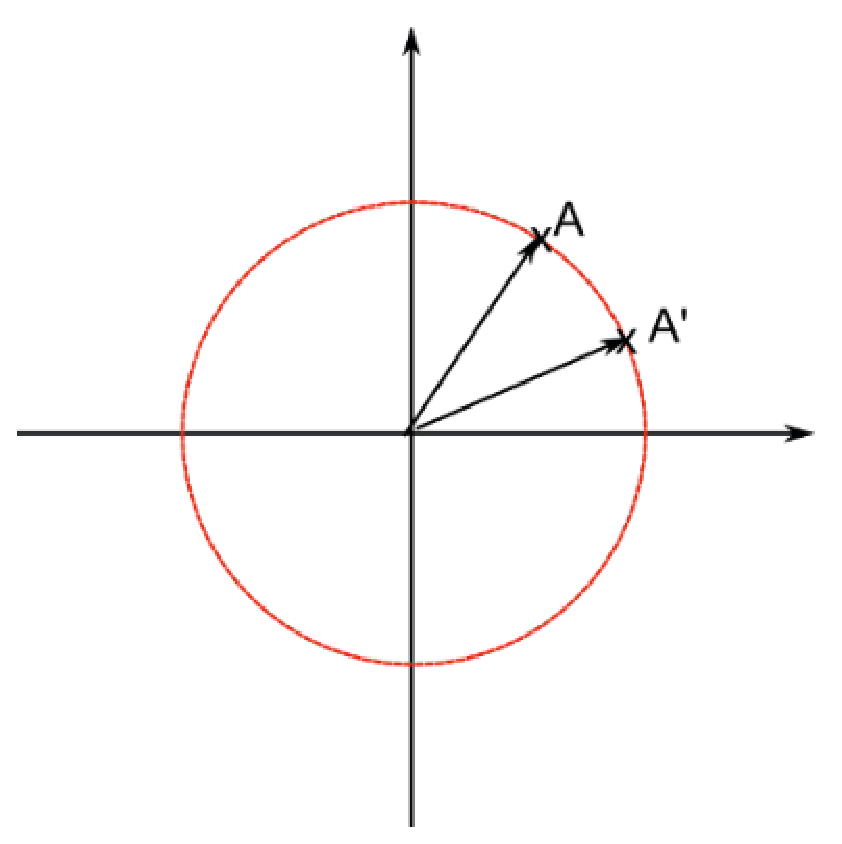
\includegraphics[scale=0.35]{fig3_4.eps}
		\figcaption{单位圆绕圆心旋转任意角度都不变}
	}

数学中除了几何图形之外还有好多别的都有对称性. 例如,对于向量, 我们可以考虑所有让向量长度不变的变换构成的集合. 看出本节开头对称性定义的普遍性了没? 对称性就是变换下的不变性. 非常幸运, 搞数学的早已建立了群论, 它可以研究所有类型的对称性\mpar{历史上数学家们建立群论最初是为了描述方程的对称性}.

为了让精确描述对称性的工具 --- 群的定义来的自然一点, 我们把对称性的定义用数学语言精炼一下:
\begin{itemize}
	\item 对某物什么也不做(比如转个$0^\circ$)当然也是对称变换(按照我们的对称性定义), 因此任何群都需要包含一个恒等变换(恒等元). 在上面的例子里, 恒等元就是旋转$0^\circ$.
	
	\item 对某物先做变换再做逆变换的结果必须等于啥也不做. 因此对于群中的任意元素(简称群元), 必须有相应的逆元素. 按定义, 先做变换再做逆变换等于恒等变换. 例如先转$90^\circ$再转$-90^\circ$(先逆针再顺针转)与旋转$0^\circ$相同.
	
	\item 先做一个对称变换再做一个对称变换, 总体效果必须还是对称变换. 例如先旋转$90^\circ$再转$180^\circ$等于直接转$270^\circ$, 后者也是对称变换. 对称变换的这个性质称为封闭性.
	
	\item 对称变换之间必须满足结合律. 例如先转$90^\circ$再转$40^\circ$再转$110^\circ$与先转$130^\circ$再转$110^\circ$相同, 先转$90^\circ$再转$150^\circ$也一样. 用符号表示更加清楚:
	\begin{equation}\label{equ3.1}
	R(110^\circ) R(40^\circ) R(90^\circ) = R(110^\circ)\bigg( R(40^\circ)R(90^\circ) \bigg) = R(110^\circ) R(130^\circ)
	\end{equation}
	\begin{equation}\label{equ3.2}
	R(110^\circ) R(40^\circ) R(90^\circ) = \bigg( R(110^\circ) R(40^\circ) \bigg) R(90^\circ) = R(150^\circ) R(90^\circ)
	\end{equation}
	这个性质称为{\bf 结合律}.
	
	\item 我们要有规定两个群元(对称变换)怎样合体的规则, 它是个{\bf 二元运算}(两个群元合体成一个), 我们称它为{\bf 群乘法}. 
	
	在上面的例子里, 旋转变换的标准表示方法是用旋转矩阵\mpar{旋转矩阵见附录A.2.}, 两个群元(两个旋转矩阵, 或两个旋转操作)合体的规则是线性代数里的矩阵乘法. 同样的变换经常有不同的表示方法\mpar{例如, 二维平面旋转还可以用单位复数描述, 相应的群乘法是复数乘法. 稍后就讨论这一点.}, 群论非常系统性地概括了所有形式. 群论的分支 --- {\bf 表示论}就是研究相同变换的不同描述方式的, 我们在\ref{sec3.5}节学习表示论.
\end{itemize}

\ 

我们把上述群与对称变换的特征用严谨的数学语言表达, 再将它们提升为公理, 满足这些公理的数学结构就是一个群. 数学系的群论书可能更喜欢在开头就从天上掉下来这些公理. 必须指出满足群公理的结构可能是超级抽象的, 但我们现在只关注上面例子里的旋转变换那样的群. \sout{因为我们是物理系的, 而且这是本物理书}

\ 

(我们通过对称变换的性质导出的)群公理\mpar{别担心怎么才能根据这些公理凑出一个群来. 搞物理的往往是从某个变换出发, 考察它是否符合群公理, 如果是\sout{经常是}那么就可以应用群论来解决问题.}: 

一个群就是一个集合$G$加上一个定义在$G$上的二元运算(群乘法)$\circ$, 当然$(G, \circ)$还要满足以下公理: 
\begin{itemize}
	\item 封闭性: 对于任意$g_1, g_2 \in G, g_1 \circ g_2 \in G$
	
	\item 单位元: 存在单位元$e \in G$使得对于所有$g \in G, g\circ e = g = e \circ g$
	
	\item 逆元: 对于任意$g \in G$, 存在相应的逆元$g^{-1} \in G$使得$g \circ g^{-1} = e = g^{-1} \circ g$
	
	\item 结合律: 对于任意$g_1, g_2, g_3 \in G, g_1 \circ (g_2 \circ g_3) = (g_1 \circ g_2) \circ g_3$ 
\end{itemize}

总结: 某物体在一些变换下保持不变, 这些变换组成\footnote{我在想这里该用`构成'还是`组成', 后来我觉得无所谓, 因为这不是初中化学...(分子构成物质, 元素组成物质...) --- 译者(SI)}的集合叫做对称群. 对于Minkowski时空, Minkowski度规\mpar{复习一下, Minkowski度规就是在Minkowski空间中用来计算距离和长度的工具, 见第二章.}在变换下保持不变, 相应的对称群称为Poincare群.

要注意群的定义完全与变换的物体是啥没有关系. 我们可以脱离特定物体而只研究对称变换本身, 群的定义将变换从物体中`提取'出来了. 这是非常有用的, 许多不同事物具有同样或同类的对称性. 群论让我们不用管变换的物体(圆还是正方形), 只研究变换(例如旋转)的普遍性质.







%!TEX encoding = UTF-8 Unicode

%----------------------------------------------------------------------------------------
%	CHAPTER 4
%----------------------------------------------------------------------------------------

\chapterimage{chapter_head_1.pdf} % Chapter heading image

\chapter{The Framework 框架/参考系}
这一章的基本思路是,我们要在尽可能少的使用\emph{某些东西}的前提下,得到正确的关于自然的方程。\emph{某些东西}是什么?有一件事是确定的:它不应该在 Lorentz 变换下改变,否则我们会在不同的参考系下得到不同的自然规律。在数学意义上,这意味着我们寻找的这个东西是个标量,依照洛伦兹群的 \( (0,0) \) 表示作变换。考虑到自然总依简单而行,这足以让我们导出关于自然的方程了。

%flag The equations of nature


%!TEX encoding = UTF-8 Unicode

\part{The Equations of Nature 自然界的方程}

%!TEX encoding = UTF-8 Unicode

%----------------------------------------------------------------------------------------
%	CHAPTER 1
%----------------------------------------------------------------------------------------

\chapterimage{chapter_head_1.pdf} % Chapter heading image

\chapter[测量]{Measuring Nature 测量}\label{chap5}

我们现在已经发现了对称性与守恒量之间的关系了,那么我们接下来就可以利用这种联系。用更专业的话说,Noether定理建立了对称变换的生成元与一个守恒量之间的联系。我们本章将利用这种联系。

守恒量常常被物理学家们用来描述物理系统,因为无论这个系统经历了怎样复杂的变化,守恒量都是一样的。比如,物理学家们为了描述一个实验会使用动量,能量或角动量。Noether定理提示我们了一个方向和一个至关重要的想法:我们在挑选哪些量我们用来描述自然的时候,我们实际上在看伴随着其对应的生成元:

\begin{align}
\text{物理量}\Rightarrow\text{对应对称性的生成元}
\end{align}

我们会看到,这种选择会自然地引导我们给出给出量子理论。

\section[量子力学中的算符]{Operators of Quantum Mechanics 量子力学中的算符}\label{sec5.1}

{\it 惯例上用一个尖帽子$\hat{O}$来表示一个算符}

拉格朗日量在空间平移操作的生成元的作用下不变导致我们得出动量守恒。因此,我们可以得到
\[\text{动量}\hat{p}_i\to\text{空间平移操作的生成元} - i\partial_i \]

类似的,时间平移的生成元带来的不变形给出我们能量守恒,也就是
\[\text{能量}\hat{E}\to\text{时间平移操作的生成元} - i\partial_0 \]

没有关于``位置守恒''的对称性,所以位置并没有伴随生成元,我们有\mpar{或者说,我们可以观察守恒量与对应的推动下的不变性。注意到我们在\ref{sec4.6}节中得到的非相对论性Galilei推动下的守恒量是从非相对论性的拉格朗日量得出来的。统一,我们可以对相对论性拉格朗日量做一样的事情,得到守恒量$i\vec{p}-\vec{x}E$。相对论性能量由$E=\sqrt{m^2+p^2}$给出。在相对论性极限$c\to\infty$下,我们有$E\approx m$,并且,Lorentz推动下的守恒量回到我们的道德Galilei推动的结果。因此,粒子理论的守恒量为$M_i = (tp_i-x_iE)$。推动的生成元(见\eqref{eq3.240},其中$K_i = M_{0i}$)为$K_i = i(x^0\partial_i-x_i\partial_0)$。比较两者,其中$x_0=t$,给出$M_i = (tp_i-x_iE)\leftrightarrow K_i = i(t\partial_i-x_i\partial_0)$。因此,利用我们之前的选择,很直观的我们有位置:$\hat{x}_i\to x_i$}
\[\text{位置}\hat{x}_i\to x_i \]

我们现在利用算符给出了我们在描述自然的理论中使用的物理量。接下来很合理的我们就需要问:这些算符作用在什么上面?它们是如何与实验中我们做的测量联系起来的呢?我们下一章将会仔细的讨论这件事情,在这里我们只需要知道我们的物理量,也就是算符,是作用在{\it 一些东西}上的。让我们暂时继续用抽象的概念理解算符作用在什么伤。我们叫它$\Psi$,我们后面会探究这个{\it 一些东西}是什么鬼。

现在,我们可以去得到一些非常重要的\mpar{如果你完全不了解量子力学,为什么这些简单地式子会如此重要对你来说会看起来比较奇怪。你也许听说过Heisenberg不确定性原理。在第\ref{sec8.3}节,我们会更进一步的研究量子力学的形式与结构,然后我们就可以看到这个方程告诉我们我们不能够一任意精度同时测量一个粒子的动量和坐标。我们的物理量的解释是算符的测量,而这个方程告诉我们先测量动量再测量位置与先测量位置再测量动量是完全不一样的。}量子力学的方程了。就像上面已经解释过的那样,我们假定我们的算符作用在抽象的$\Psi$上。于是我们就有
\begin{align}
\begin{split}
[\hat{p}_i,\hat{x}_k]&\Psi = (\hat{p}_x\hat{x}_j)\Psi = (\partial_i \hat{x}_j-\hat{x}_j\partial_i)\Psi\\
\underbrace{=}_{\text{莱布尼兹律}}& (\partial_i\hat{x}_j)\Psi + \cancel{\hat{x}_j(\partial_i\Psi)} - \cancel{\hat{x}_j(\partial_i\Psi)} \underbrace{=}_{\text{因为}\partial_i\hat{x}_j = \frac{\partial x_j}{\partial x_i}} i\delta_{ij}\Psi
\end{split}
\end{align}

这个方程对任意的$\Psi$都成立,因为我们没有对$\Psi$做任何假设,因此我们可以不考虑它\mpar{如果这对你来说比较罕见,注意我们可以把{\bf 每}一个矢量方程都写成只包含数的形式。比如,牛顿第二定律$\vec{F} = m\vec{\ddot{x}}$,可以对于任意矢量$\vec{C}$写出$\vec{F}\vec{C} = m\vec{\ddot{x}}\vec{C}$。不仅如此,如果对于任意的$\vec{C}$都成立,那么一直把这个$\vec{C}$写着也就没什么意义了。}而直接的写出
\begin{align}
[\hat{p}_i,\hat{x}_j] = i\delta_{ij}
\end{align}

\subsection[自旋与角动量]{Spin and Angular Momentum 自旋与角动量}\label{sec5.1.1}

上一章的第\ref{sec4.5.4}节中我们看到,只是对标量理论来说,旋转不变形带来的守恒量有两个部分,而这个第二部分则对应了轨道角动量,我们把它称为{\bf 无限}维的轨道角动量生成元的表示。$\hat{L}_i\to\text{转动生成元(无限维表示)}i\tfrac{1}{2}\epsilon_{ijk}(x^j\partial^k-x^k\partial^j)$。类似的我们 把第一部分称作自旋,对应{\bf 有限}维度的生成元\mpar{记得这就是从场的分量的混杂的不变性带来的守恒量,因此是有限维的表示。}的表示。
\[\text{自旋}\hat{S}_i\to\text{转动生成元(有限维表示)}S_i \]
如前面\eqref{eq4.30}解释过的那样,$S_{\mu\nu}$和转动算符生成元$S_i$的关系为$S_i = \tfrac{1}{2}\epsilon_{ijk}S_{jk}$。

比如,当我们考虑自旋$\tfrac{1}{2}$场的时候,我们需要用到我们在节\ref{sec3.7.5}中得到的二维表示:
\begin{align}
\hat{S}_i = i\frac{\sigma_i}{2}
\end{align}
其中$\sigma_i$是Pauli矩阵。我们会在节\ref{sec8.5.5}学习了如何利用我们本章得到的这些算符之后回到这一有趣而奇怪的类型的角动量。时刻注意,只有这两部分的{\bf 和}是守恒的。

\section[量子场论的算符]{The Operators of Quantum Field Theory 量子场论的算符}\label{sec5.2}

场论的最重要的客体当然就是{\bf 作为时空位置的函数}\mpar{这里,$x = x_0,x_1,x_2,x_3$,包含时间$x_0=t$。}的场了$\Phi = \Phi(x)$。我们接下来希望描述时空上的一个点发生的相互作用,从而我们需要考虑动力学变量$\pi = \pi(x)$的密度,而不是其其总量$\Pi = \int d^3x\pi(x)\neq\Pi(x)$。

我们上一章发现了在奇异不变性下场自己$\Phi\to\Phi-i\epsilon$产生了一种新的守恒量,称为共轭动量$\Pi$。就像我们上一章做的那样,我们用对应的生成元来表示共轭动量密度\eqref{eq4.59}。
\[\text{共轭动量密度}\pi(x)\to\text{关于场自己的平移的生成元:}-i\frac{\partial}{\partial\Phi(x)} \]
我们后面会看到量子场论与这里处理的稍稍不同,而且我们这里的实际上已经足够了。

\[\delta S\to\delta S' = \delta S+\int_{t_1}^{t_2}dt\frac{d}{dt}\delta G = \delta S+ \!\!\!\!\!\!\!\!\!\!\!\!\!\!\!\! \underbrace{\frac{\partial G}{\partial q}\delta q|_{t_1}^{t_2}}_{=0\text{ because }\delta q(t_1)=\delta q(t_2)=0} \]


%!TEX encoding = UTF-8 Unicode

%----------------------------------------------------------------------------------------
%	CHAPTER 6
%----------------------------------------------------------------------------------------

\chapterimage{chapter_head_1.pdf} % Chapter heading image

\chapter[自由场理论]{Free Theory 自由场理论}\label{chap6}

在这章中,我们建立自由的体系的物理理论,也就是说无相互作用的情况下的对称性给出的场\mpar{尽管我们这里针对的是场,后面会看到这里得到的方程同样可以用来处理粒子}。我们会
\begin{itemize}
\item 利用Lorentz群的$(0,0)$表示给出Klein-Gordon方程
\item 利用Lorentz群的$(\tfrac{1}{2},0)\oplus(0,\tfrac{1}{2})$表示给出Dirac方程
\item 利用Lorentz群的矢量$(\tfrac{1}{2},\tfrac{1}{2})$表示给出Proca方程,在无质量极限下退化到著名的Maxwell方程组
\end{itemize}

\section[Lorentz协变性与不变量]{Lorentz Covariance and Invariance Lorentz协变性与不变量}\label{sec6.1}

在下面的章节中,我们会得到粒子物理的标准模型- 这是我们拥有的最好的物理理论 -中的运动方程。我们期待这些房产在所有的惯性系中看起来都一样,因为如果不这样的话,我们就会对每一个可能的参考系都有各自的方程。狭义相对论指出并没有一个特别的参考系,所以这一点是没有意义的。这个术语被称为{\bf Lorentz协变性}。一个Lorentz协变的物体是说它按照某一种给定的Lorentz群来进行变换。比如说,矢量$A_\mu$,通过$\left(\frac{1}{2},\frac{1}{2}\right)$表示来进行变换,因此是Lorentz协变的;这其实是说,$A_\mu\to A'_{\mu'}$,但实际上这两个指代同一个东西,并不是完全不同的。另一方面,比如说,$A_1+A_3$就不是Lorentz协变的,因为它不按照Lorentz群的某种表示来变换。但这并不是说我们不知道它是如何变换的,因为它的变换规律从$A_\mu$的变换规律里面可以简单地得出,但是在不同的惯性系中它看起来完全不一样。在一个``推动''的参考系中它看起来或许像$A_2+A_4$。只涉及到Lorentz协变的东西的方程被称为Lorentz协变方程,比如
\[A_\mu+7B_\mu+C_\nu A^\nu D_\mu = 0 \]
就是一个Lorentz协变方程,因为在另一个参考系中,它看起来就是
\[A_\mu+7B_\mu+\underbrace{C_\nu A^\nu}_{\mathclap{=\text{一个Lorentz标量,根据$(0,0)$表示来进行变换}}} D_\mu = A'_\mu+7B'_\mu+C_\nu A^\nu D'_\mu = 0 \]
我们看到它看起来是一样的。一个只有部分是这样的东西的方程,一般来说并不是Lorentz协变的,从而在另一个惯性系里面就会不一样。

为了确定我们只使用Lorentz{\bf 协变}的方程,我们需要要求作用量$S$是Lorentz{\bf 不变}的。这是说它只能包含那些在参考系变换下保持不变的成分。换句话说,作用量里面只可以包含Lorentz变换下不变的部分。从作用量$S$中我们可以得到运动方程\mpar{回忆一下我们保持作用量最小以及得来的欧拉-拉格朗日方程,就是对系统的运动方程}。如果现在$S$依赖于参考系,也就是说得到的运动方程不再是Lorentz协变的了。

就像我们之前一章讨论的那样,我们可以用更严格的约束条件来要求拉格朗日量应该是不变的,因为这样的话作用量也就肯定是不变的了。

\section[Kelin-Gordon 方程]{Kelin-Gordon Equation Kelin-Gordon 方程}

我们现在开始考虑最简单的情况:标量,其按照Lorentz群的$(0,0)$表示变化。我们需要找一个对应的拉格朗日量来确定标量的运动方程。一个符合我们限制的一般的拉格朗日量第\mpar{在\ref{sec4.2}节中有所讨论:我们只考虑$0, 1$和$2$阶的$\Phi$。只考虑最低可能的导数项的原因在后面就会说明。}是:

\begin{align}
\mathcal{L} = A\Phi^0+V\Phi+C\Phi^2+D\partial_\mu\Phi+E\partial_\mu\Phi\partial^\mu\Phi+F\Phi\partial_\mu\Phi
\end{align}
首先,需要注意我们考虑的是拉格朗日量密度$\mathcal{L}$而不是$L$本身,然后我们的物理理论可以从作用量
\begin{align}
S = \int dx\mathcal{L}
\end{align}
得出,其中$dx$可以理解为对时间和空间的积分。因此,诸如$\Phi\partial_\mu\partial^\mu\Phi$的项实际是没必要的,因为它等效于$\partial_\mu\Phi\partial^\mu\Phi$,从分部积分就可以直接地看到这一点\mpar{很直接的,边界项会被小区,因为在远处场很小。值得注意的是,这是由于我们物理里面的速度是有上限的(第\ref{sec2.3}节)。因此,很远处的场对于有限远的$x$位置的场不会有影响}。

不仅如此,Lorentz{\bf 不变形}要求拉格朗日量必须是一个标量。因此,所有奇数阶的$\partial_\mu$,比如$\partial_\mu\Phi$是禁止的。值得一提的是,如果常数,比如$a, c$,有一个Lorentz指标的话,这说明这些常数是一个$4$-矢量,标定了时空的方向从二破坏了空间的各向同性的要求。我们实际上可以忽略常数项,也就是$A=0$,因为我们的物理理论需要从欧拉-拉格朗日方程中得到,因此一个常数项对运动方程没有影响\mpar{考虑\eqref{eq4.10}:$\frac{\partial{\mathcal{L}}}{\partial\Phi}-\partial_\mu\left(\frac{\partial{\mathcal{L}}}{\partial(\partial_\mu\Phi)}\right)$,因此$\mathcal{L}\to\mathcal{L}+A$中的常数项$A$并不改变任何东西:$\frac{\partial({\mathcal{L}}+A)}{\partial\Phi}-\partial_\mu\left(\frac{\partial({\mathcal{L}}+A)}{\partial(\partial_\mu\Phi)}\right) = \frac{\partial{\mathcal{L}}}{\partial\Phi}-\partial_\mu\left(\frac{\partial{\mathcal{L}}}{\partial(\partial_\mu\Phi)}\right)$}。











%!TEX root = ..\main.tex
%!TEX encoding = UTF-8 Unicode

%——————————————————————————————————————————————————————————-
%	CHAPTER 7
%——————————————————————————————————————————————————————————-
\newcommand\ue{\mathrm e}
\newcommand\sutw{$\mathcal{SU}(2)$}
\newcommand\suth{$\mathcal{SU}(3)$}
\newcommand\uo{$\mathcal{U}(1)$}
\newcommand\spint{自旋$\frac{1}{2}$}
\chapterimage{chapter_head_1.pdf} % Chapter heading image

\chapter[相互作用理论]{Interaction Theory\quad 相互作用理论}\label{chap7}

\section*{Summary\quad 总结}
在这一章中我们将导出不同的场之间的相互作用。这使得我们能够,例如,描述电子是如何和光子作用的%
\mpar{从另外一个视角看:电子(\spint 且有质量)场如何和光子(自旋为$1$)场作用。}。

内禀对称性,或者这里叫做规范%
\mpar{马上就会解释这个奇怪的名字}
对称性,能指引我们得到拉格朗日量的正确形式。我们将从局域%
\mpar{这意味着不仅仅是一个$\ue^{\ri\alpha}$,而是在每一个时空点上作用一个不同的因子,数学上写作$\ue^{\ri\alpha(x)}$。或者这样说:变换参数$\alpha=\alpha(x)$现在是$x$的函数,在不同的时空点上有不同的值。}%
$\mathcal{U}(1)$对称性出发来得到拉格朗日量
\[
{\mathscr L} = -m\bar\Psi\Psi+\ri\bar\Psi\gamma_\mu\partial^\mu\Psi + A_\mu\bar\Psi\gamma^\mu\Psi + \partial^\mu A^\nu\partial_\mu A_\nu - \partial^\mu A^\nu \partial_\nu A_\mu \text{,}
\]
即{\bf 量子电动力学(quantum electrodynamics)}的拉格朗日量。这个拉格朗日量描述了有电荷有质量的场和无质量自旋为$1$的场(光子场)之间的相互作用。在排除了形如$mA_\mu A^\mu$的“质量项”后(这和用$A_\mu$来描述的光子是无质量的实验事实相符),拉格朗日量只有这样才是局域$\mathcal{U}(1)$不变的%
\mpar{译注:应该为“只有这样才是且仅是”。}%
。利用 Noether 定理,我们能从\uo 对称性中导出一个新的守恒量,它常被解释为{\bf 电荷(electric charge)}。

接下来是$\mathcal{SU}(2)$对称性。引入一个二分量的{\bf 二重态(doublet)}
\[
\bar\Psi : = \begin{pmatrix}
\bar\psi_1 & \bar\psi_2
\end{pmatrix}\text{,}
\]
这样一个二重态场中包含了两个\spint 场,例如,电子和电子中微子场在$\mathcal{SU}(2)$的“旋转”下相互转换。

我们可以使用二重态记号写下局域$\mathcal{SU}(2)$不变的拉格朗日量%
\mpar{$W_j^{\mu\nu}$这玩意会通过三个$W_j^\mu$定义,就像从\uo 规范场$A^\mu$定义$F_{\mu\nu}$一样。}
\[
{\mathscr L} = \ri\bar\Psi\gamma_\mu\partial^\mu\Psi + \bar\Psi\gamma_\mu\sigma_j W_j^\mu\Psi - \frac{1}{2}(W_{\mu\nu})_i(W^{\mu\nu})_i \text{,}
\]
其中包含了三个自旋为$1$的场$W_j^\mu$。由于\sutw 群的生成元有三个基$J_i=\sigma_i/2$,所以我们需要三个场来保证拉格朗日量是局域\sutw 不变的。我们将看到局域\sutw 对称性仅当形如$m\bar\Psi\Psi$、$mW_\mu W^\mu$的质量项(其中质量$m$是任意给定{\bf 矩阵})不存在时才有可能实现,这是因为$\Psi$现在是二分量对象了。所以此时不仅自旋为$1$的场$W_j^\mu$得是无质量的了,\spint 场也一样。另外一种可能是两个\spint 等质量场,但是它被实验否决了:电子质量远大于电子中微子质量。除此之外,我们从实验知道三个自旋为$1$的场$W_j^\mu$不是无质量的。这常解释成\sutw 对称性被破缺了。

这是随后被引入的{\bf Higgs 机制(Higgs formalism)}的想法来源。这个机制能使我们得到一个包含质量项的\sutw 不变的拉格朗日量。它通过引入一个与零自旋场,即 Higgs 场,的相互作用来达成目标。相同的机制使我们能给\spint 场加上任意的质量项以与实验相符。最后的相互作用拉格朗日量描述了一种新的相互作用:{\bf 弱相互作用(weak interaction)},由三个%
\mpar{准确的讲:我们从${\mathcal U}(1)\otimes{\mathcal SU}(2)$对称破缺到\uo 。这个过程产生了三个有质量矢量 bosons:$W^+$、$W^-$、$Z$,和一个无质量矢量 bosons:$\gamma$光子。所以说为什么常讲电磁学(来自\uo 对称性)和弱相互作用理论(来自\sutw )是统一的。一开始的\uo 对称性和最后留下来的\uo 对称性不是一个东西。光子和$Z$Bosons可以看做是两个矢量Bosons的线性组合,常记做$B$和$W^3$,用以使拉格朗日量具有局域\uo ($B$波色子)和\sutw ($W^1$、$W^2$、$W^3$-bosons)不变性。}%
有质量自旋为$1$的场:$W^+$、$W^-$和$Z$,作为传播媒介。利用 Noether 定理,我们能从\sutw 对称性得到一个新的守恒量:{\bf 同位旋(isospin)},它相当于于电磁相互作用中的电荷,是弱相互作用中的荷。

最后,我们将考虑内禀\suth 对称,它将会将我们能描述一类新的相互作用,{\bf 强相互作用(strong interaction)},的拉格朗日量。为此我们将引入一个三重态
\[
Q = \begin{pmatrix}
q_1 \\
q_2 \\
q_3
\end{pmatrix}\text{,}
\]
在\suth 下变换,包含三个\spint 场。这三个\spint 场被解释为有不同{\bf 颜色(color)}的{\bf 夸克(quarks)},这是电磁作用中的电荷、或者弱作用中的同位旋在强相互作用中的对应物。一样,质量项是被禁止的,但这次和实验结论一致:8个相应的 bosons%
\mpar{数字8源于\suth 的生成元有8个基。}%
,称为胶子,是无质量的%
\mpar{作为补充,我们从实验知道\suth 的三重态中的场有相同的质量。这是个好消息,因为局域\suth 对称性禁止形如$m\bar QQ$这样带有任意质量矩阵$m$的项存在,但允许$\bar Q \begin{pmatrix}m&0\\ 0&m\end{pmatrix} Q$这样一项,这代表三重态里的项有相同的质量。由此局域\suth 不变性不会在拉格朗日量的质量项上造成新的障碍,\suth 对称也不没有被破缺。}%
。根据实验我们知道只有夸克(\spint )和胶子(自旋为$1$)携带颜色。最后,拉格朗日量的结果是
\[
{\mathscr L} = -\frac{1}{4}F_{\alpha\beta}^A F_A^{\alpha\beta} + \bar Q(\ri D_\mu\gamma^\mu - m)Q \text{,}
\]
咱仅仅引用一下\sout{装个逼},因为推导太繁琐了,并且和我们之前做过的完全类似。

给总结来总结一下:
\begin{table}[htbp]
\begin{tabular}{ccccccc}
 \uo & $\rightarrow$ & 1个规范场 & $\rightarrow$ & {\bf 无质量}光子 & $\rightarrow$ & 电荷 \\
 \sutw & $\rightarrow$ & 3个规范场 & $\rightarrow$ & {\bf 有质量}W- 和 Z-bosons (需要 Higgs ) & $\rightarrow$ & 同位旋 \\
 \suth & $\rightarrow$ & 8个规范场 & $\rightarrow$ & {\bf 无质量}胶子 & $\rightarrow$ & 色荷
\end{tabular}
\end{table}

\section[$\mathcal{U}(1)$相互作用]{$\mathcal{U}(1)$ Interaction\quad $\mathcal{U}(1)$相互作用}\label{sec7.1}
为了得到拉格朗日量中正确的相互作用项,我们得使用内禀对称性,或者称作{\bf 规范对称性(gauge symmetries)}。规范对称这个叫法有一些历史上的原因,和我们现在要讨论的东西之间关系不是太大。Weyl 曾尝试将电磁学%
\mpar{Frank Wilczek. Riemann-einstein structure from volume and gauge symmetry. Phys. Rev. Lett., 80:4851–4854, Jun 1998. doi: 10.1103/PhysRevLett.80.4851}%
“作为时空对称性的结果,特别是在局域尺度变换下的对称性”。将其称作规范对称性是有原因的,因为它意味着,例如,我们能任意改变用于定义长度标准的铂金尺(用来规范\footnote{译注:没有规矩,不成方圆。线长是某个线性空间中的某种范数,将改变线长的定义的变换,称作规范变换,应当是一个合理的称呼。关于 gauge 这个词的命名以及为何翻译成“规范”,可以参见 曹则贤 . Norm and Gauge[J]. 物理, 2013, 42(11): 815-819. }实验中测长的仪器),而不改变物理。这个尝试没有成功,但稍晚些时候,Weyl 找到了能正确导出电磁学的对称性,并仍用这个词来命名。

\subsection{\spint 自由场的内禀对称性}\label{sec7.1.1}
再来看一眼用来导出自由\spint 理论的拉格朗日量(\ref{eq:6.16}式)
\begin{equation}
{\mathscr L}_\text{Dirac} = -m\bar\Psi\Psi +\ri\bar\Psi\gamma_\mu\partial^\mu\Psi = \bar\Psi(\ri\gamma_\mu\partial^\mu-m)\Psi
\end{equation}
它是在 Lorentz 对称性的要求下导出的,但如果我们仔细观察它,能发现这个拉格朗日量中蕴含着另一个对称性。拉格朗日量在场$\Psi$的如下变换下不变
\begin{eqnarray}
\Psi &\rightarrow& \Psi' = \ue^{\ri a}\Psi \nonumber \\
\Rightarrow \bar\Psi &\rightarrow& \bar\Psi' = \Psi'^\dag \gamma_0 = (\ue^{\ri a}\Psi)^\dag \gamma_0 =\bar\Psi \ue^{-\ri a} \text{,}
\end{eqnarray}
其中负号来源于复共轭\mpar{别忘了$\bar\Psi=\Psi^\dag \gamma_0 $}%
,而$a$是一个任给实数。为了看清这一点,我们将变换后的场的拉格朗日量明确写出
\begin{eqnarray}
{\mathscr L}_\text{Dirac}' &=& -m\bar\Psi'\Psi' +\ri\bar\Psi'\gamma_\mu\partial^\mu\Psi' \nonumber\\
&=& -m(\bar\Psi \ue^{-\ri a})(\ue^{\ri a}\Psi)+\ri(\bar\Psi \ue^{-\ri a})\gamma_\mu\partial^\mu\Psi(\ue^{\ri a}\Psi) \nonumber\\
&=& -m\bar\Psi\Psi \underbrace{\ue^{-\ri a}\ue^{\ri a}}_{\mathclap{=1}} + \ri\bar\Psi\gamma_\mu\partial^\mu\Psi \underbrace{\ue^{-\ri a}\ue^{\ri a}}_{\mathclap{=1}} \nonumber\\
&=& -m\bar\Psi\Psi +\ri\bar\Psi\gamma_\mu\partial^\mu\Psi ={\mathscr L}_\text{Dirac}
\end{eqnarray}
其中我们利用了$\ue^{\ri a}$仅是一个复数这一点来将它自由前后挪动%
\mpar{技术上讲:一个复数和所有矩阵对易,例如$\gamma_\mu$。}%
。回忆我们在第\ref{chap3}章中曾讲过的,任何单位复数(能写作$\ue^{\ri a}$的形式)构成了一个\uo 群,由此可以将我们刚才发现的事实用数学语言表达出来:拉格朗日量是\uo 不变的。由于它丝毫不涉及时空的变换而只改变场自身,所以说这是一个内禀对称性。猛地一看,这玩意还挺萌的,但好像没什么用。不要走开,稍后的节目会告诉你它有多精彩!

现在咱再来钻深一点。我们刚展示了,给我们的场乘一个任意单位复数什么都不会改变。这个对称变换$\Psi \rightarrow \Psi' = \ue^{\ri a}\Psi$叫做{\bf 全局(global)}变换,因为我们在每一个点$x$给场$\Psi=\Psi(x)$乘上了一个相同的因子$\ue^{\ri a}$。

所以说,为什么一个时空点的相位因子会和另一个时空点的相关呢?一个点的选取不应该瞬间改变整个宇宙的情况。这是挺奇怪的,因为正如\ref{sec2.4}节中所述,狭义相对论告诉我们没有信息能比光传播得更快。而全局对称性选择会瞬间应用到在整个宇宙中的每一个点上%
\footnote{译注:引入局域规范的另一种讲法是,我们不能保证外星人里物理学家和我们选取同一套规范(这里的$a$是可以随意选取的,但是必须要选取一个才能得到完整的理论。$a$的选取被称为规范的选取),但是物理定律不应该有区别。}%
。

让我们来检查一下,如果给每一个时空点变换一个不同的因子$a=a(x)$,拉格朗日量是不是还是不变的。这叫做{\bf 局域(local)}变换。

我们作变换
\begin{eqnarray}
\Psi &\rightarrow& \Psi' = \ue^{\ri a(x)}\Psi \nonumber \\
\Rightarrow \bar\Psi &\rightarrow& \bar\Psi' = \Psi'^\dag \gamma_0 = (\ue^{\ri a(x)}\Psi)^\dag \gamma_0 =\bar\Psi \ue^{-\ri a(x)} \text{,}
\end{eqnarray}
现在$a=a(x)$依赖于坐标了,我们得到变换后的拉格朗日量%
\mpar{可能你会好奇包含全部可能导数项的拉格朗日量(由简洁性的要求被忽略)是不是局域\uo 不变的:${\mathscr L} = -m\bar\Psi\Psi +\ri\bar\Psi\gamma_\mu\partial^\mu\Psi+\ri(\partial^\mu\Psi)\gamma_\mu\Psi$。你可以检查一下,这个拉格朗日量自然是局域\uo 不变的,但注意第二项和第三项之和为零:$\ri\bar\Psi\gamma_\mu\partial^\mu\Psi+\ri(\partial^\mu\Psi)\gamma_\mu\Psi \underbrace{=}_{\mathclap{\text{分部积分}}} \ri(\partial^\mu\Psi)\gamma_\mu\Psi-\ri(\partial^\mu\Psi)\gamma_\mu\Psi = 0 $。包含了全部可能导数的正确拉格朗日量的两导数项间必须有一个相对负号:${\mathscr L_\text{Dirac}} = -m\bar\Psi\Psi +\ri\bar\Psi\gamma_\mu\partial^\mu\Psi-\ri(\partial^\mu\Psi)\gamma_\mu\Psi$,故它并{\bf 不}是局域\uo 不变的。
}
\begin{eqnarray}
{\mathscr L}_\text{Dirac}' &=& -m\bar\Psi'\Psi' +\ri\bar\Psi'\gamma_\mu\partial^\mu\Psi' \nonumber\\
&=& -m(\bar\Psi \underbrace{\ue^{-\ri a})(\ue^{\ri a}}_{\mathclap{=1}}\Psi)+\ri(\bar\Psi \ue^{-\ri a(x)})\gamma_\mu\partial^\mu\Psi(\ue^{\ri a(x)}\Psi) \nonumber\\
&=& -m\bar\Psi\Psi + \ri\bar\Psi\gamma_\mu\partial^\mu\Psi \underbrace{\ue^{-\ri a}\ue^{\ri a}}_{\mathclap{=1}} \underbrace{+}_{\mathclap{\text{莱布尼兹律}}} \ri(\ue^{-\ri a(x)}\bar\Psi)\gamma_\mu\Psi(\partial^\mu\ue^{\ri a(x)}) \nonumber\\
&=& -m\bar\Psi\Psi +\ri\bar\Psi\gamma_\mu\partial^\mu\Psi + \ri^2(\partial^\mu a(x))\bar\Psi\gamma_\mu\Psi \ne {\mathscr L}_\text{Dirac}
\label{eq:7.5}
\end{eqnarray}
由于莱布尼兹律导致了一个额外的项,所以说我们的拉格朗日量在局域\uo 对称变换下不是不变的。但按照上面所讨论的,拉格朗日量应该是局域不变的,在这里却不是。这里有一些事情可做,但我们得先研究另一种对称性。
\subsection{自旋为$1$自由场的内禀对称性}\label{sec7.1.2}
接下来,来看看自旋为一的粒子\mpar{对比\ref{eq:6.25}式,注意我们为了简明起见而丢掉的$\frac{1}{2}$因子}
\begin{equation}
{\mathscr L}_\text{Proca} = \partial^\mu A^\nu\partial_\mu A_\nu - \partial^\mu A^\nu \partial_\nu A_\mu + m^2A_\mu A^\mu \text{。}
\end{equation}
这儿也能找到一个全局内禀对称性。如果我们作变换
\begin{equation}
A_\mu \rightarrow A_\mu' = A_\mu+a_\mu
\end{equation}
其中$a_\mu$为任意常数,拉格朗日量变为
\begin{eqnarray}
{\mathscr L}_\text{Proca}' &=& \partial^\mu A'^\nu\partial_\mu A_\nu' - \partial^\mu A'^\nu \partial_\nu A_\mu' + m^2A_\mu' A'^\mu \nonumber\\
&=& \partial^\mu (A^\mu+a^\nu)\partial_\mu (A_\nu+a_\nu) - \partial^\mu (A^\nu+a^\nu) \partial_\nu ( A_\mu+a_\mu) + m^2( A_\mu+a_\mu) ( A^\mu+a^\mu) \nonumber\\
&=& \partial^\mu A^\nu\partial_\mu A_\nu - \partial^\mu A^\nu \partial_\nu A_\mu + m^2( A_\mu+a_\mu) ( A^\mu+a^\mu)
\end{eqnarray}
由此我们作出结论,对于{\bf 无质量}场($m=0$),这个变换是个{\bf 全局}对称的变换。

那{\bf 局域}对称性又会怎么样呢?作变换
\begin{equation}
A_\mu \rightarrow A_\mu' = A_\mu+a_\mu(x)
\end{equation}
{\bf 无质量}的拉格朗日量变成
\begin{eqnarray}
{\mathscr L}_\text{Maxwell}' &=& \partial^\mu A'\nu\partial_\mu A_\nu' - \partial^\mu A'\nu \partial_\nu A_\mu' \nonumber\\
&=& \partial^\mu (A^\mu+a^\nu(x))\partial_\mu (A_\nu+a_\nu(x)) - \partial^\mu (A^\nu+a^\nu(x)) \partial_\nu ( A_\mu+a_\mu(x))  \nonumber\\
&=& \partial^\mu A^\nu\partial_\mu A_\nu+\partial^\mu a^\nu(x)\partial_\mu A_\nu+\partial^\mu A^\nu\partial_\mu a_\nu(x) +\partial^\mu a^\nu(x)\partial_\mu a_\nu(x) \nonumber\\
& &\quad - \partial^\mu A^\nu \partial_\nu A_\mu - \partial^\mu A^\nu \partial_\nu a_\mu(x)-\partial^\mu a^\nu(x) \partial_\nu A_\mu - \partial^\mu a^\nu(x) \partial_\nu a_\mu(x)
\end{eqnarray}
即没有内禀对称性。

然而,如果我们这样作变换$A_\mu\rightarrow A_\mu'+\partial_\mu a(x)$,我们能弄出一个局域内禀对称性来。这意味着我们加的是一个任意函数的导数,而不是一个任意函数。这会导致\footnote{\textcolor{red}{译注:原文缺少一个$(x)$}}
\begin{eqnarray}
{\mathscr L}_\text{Maxwell}' &=& \partial^\mu A'\nu\partial_\mu A_\nu' - \partial^\mu A'\nu \partial_\nu A_\mu' \nonumber\\
&=& \partial^\mu (A^\mu+\partial^\nu a(x))\partial_\mu (A_\nu+\partial_\nu a(x)) - \partial^\mu (A^\nu+\partial^\nu a(x)) \partial_\nu ( A_\mu+\partial_\mu a(x))  \nonumber\\
&=& \partial^\mu A^\nu\partial_\mu A_\nu+\partial^\mu \partial^\nu a(x)\partial_\mu A_\nu+\partial^\mu A^\nu\partial_\mu \partial_\nu a(x) +\partial^\mu \partial^\nu a(x)\partial_\mu \partial_\nu a(x) \nonumber\\
& & - \partial^\mu A^\nu \partial_\nu A_\mu - \partial^\mu A^\nu \partial_\nu \partial_\mu a(x)-\partial^\mu \partial^\nu a(x) \partial_\nu A_\mu - \partial^\mu \partial^\nu a(x) \partial_\nu \partial_\mu a(x) \nonumber \\
&\underbrace{=}_{\mathclap{\partial_\nu\partial_\mu=\partial_\mu\partial_\nu\text{以及重命名哑指标}}}& \partial^\mu A^\nu\partial_\mu A_\nu - \partial^\mu A^\nu \partial_\nu A_\mu = {\mathscr L}_\text{Maxwell}\label{eq:7.11}
\end{eqnarray}
所以说这里的确有一个局域内禀对称变换。这看上去也像是一个技术细节。好的,我们找到了一些局域的、内禀的对称性,然后呢?
\subsection{把奇怪的东西堆一起}\label{sec7.1.3}
总结一下咱现在都干了啥
\begin{itemize}
\item 我们发现\spint 自由场的拉格朗日量有一个全局的内禀对称性$\Psi\rightarrow\Psi' = \ue^{\ri a}\Psi$。或者这样说:\spint 自由场的拉格朗日量在全局\uo 变换下不变。
\item 这个对称性不是局域的(尽管它应当是),因为在$a=a(x)$的情况下,我们在拉格朗日量中得到如下形式的额外项(\ref{eq:7.5}式)
\begin{equation}
-(\partial_\mu a(x))\bar\Psi\gamma^\mu\Psi \text{。}
\label{eq:7.12}
\end{equation}
换言之:拉格朗日量不是局域\uo 不变的。
\item 上一节中我们发现了无质量自旋为一的场的一个局域内禀对称性
\begin{equation}
A_\mu \rightarrow A_\mu' = A_\mu +\partial_\mu a(x) \text{,}
\end{equation}
它仅当我们加上的是一个任意函数的导数$\partial_\mu a(x)$,而不是一个任意函数$a_\mu(x)$时,才是一个局域对称性。
\end{itemize}
这两坨奇怪的东西看上去真该加在一起:拉格朗日量中的一个额外项$A_\mu\bar\Psi\gamma^\mu\Psi$会变换作
\begin{equation}
A_\mu\bar\Psi\gamma^\mu\Psi \rightarrow (A_\mu+\partial_\mu a(x))\bar\Psi\gamma^\mu\Psi = A_\mu\bar\Psi\gamma^\mu\Psi + \partial_\mu a(x)\bar\Psi\gamma^\mu\Psi
\end{equation}
比较$\ref{eq:7.12}$式中的第二项\footnote{\textcolor{red}{译注:此处疑引用有误}}。拉格朗日量中这个将$\Psi$、$\bar\Psi$和$A_\mu$耦合在一起的新项,正好能干掉那个\sout{不自量力}阻挡\spint 自由场拥有局域\uo 不变性的家伙。换言之:{\bf 通过添加这个新项使得拉格朗日量局域\uo 不变。}

再来仔细研究一下这件事。首先习惯上都会在局域\uo 变换的指数上添一个常数因子$g$:$\ue^{\ri ga(x)}$。这样额外项变成
\begin{equation}
-(\partial_\mu a(x))\bar\Psi\gamma^\mu\Psi \rightarrow -g(\partial_\mu a(x))\bar\Psi\gamma^\mu\Psi \text{。}
\end{equation}
正如我们下面将看到的,这个额外的因子$g$代表一个任意的耦合常数%
\mpar{耦合常数总能告诉我们相互作用的强度是多少。这里讨论的是电磁相互作用,$g$代表着它的强度。}%
$g$。将这个新项
\[
g A_\mu\bar\Psi\gamma^\mu\Psi
\]
加到\spint 自由场的拉格朗日量上,其中$\gamma^\mu$用来保证这一项的 Lorentz 不变性,否则带有一个自由指标$\mu$的$A_\mu$和拉格朗日量密度这个标量无法匹配,另外也插入了{\bf 耦合常数(coupling constant)}%
\mpar{我们能看到这里$g$决定了$\Psi$、$\bar\Psi$和$A_\mu$耦合在一起的强度。}%
$g$。这样拉格朗日量
\[
{\mathscr L}_\text{Dirac+额外项} = -m\bar\Psi\Psi +\ri\bar\Psi\gamma_\mu\partial^\mu\Psi + g A_\mu\bar\Psi\gamma^\mu\Psi \text{。}
\]
依据$\Psi$、$\bar\Psi$和$A_\mu$局域变换的规则来变换这个拉格朗日量,得到%
\mpar{$\Psi$、$\bar\Psi$和$A_\mu$的联合变换被称作\uo 规范变换。}
\begin{eqnarray}
{\mathscr L}_\text{Dirac+额外项}' &=& -m\bar\Psi'\Psi' +\ri\bar\Psi'\gamma_\mu\partial^\mu\Psi' + g A_\mu'\bar\Psi'\gamma^\mu\Psi' \nonumber\\
&\underbrace{=}_{\mathclap{\text{见\ref{eq:7.5}式}}}&  -m\bar\Psi\Psi +\ri\bar\Psi\gamma_\mu\partial^\mu\Psi - g (\partial_\mu a(x))\bar\Psi\gamma^\mu\Psi + g A_\mu'\bar\Psi'\gamma^\mu\Psi' \nonumber \\
&=& -m\bar\Psi\Psi +\ri\bar\Psi\gamma_\mu\partial^\mu\Psi - g (\partial_\mu a(x))\bar\Psi\gamma^\mu\Psi + g (A_\mu+\partial_\mu a(x))(\ue^{-\ri ga(x)}\bar\Psi)\gamma^\mu(\ue^{\ri ga(x)}\Psi) \nonumber \\
&=& -m\bar\Psi\Psi +\ri\bar\Psi\gamma_\mu\partial^\mu\Psi - \cancel{g (\partial_\mu a(x))\bar\Psi\gamma^\mu\Psi} + g A_\mu\bar\Psi\gamma^\mu\Psi + \cancel{g (\partial_\mu a(x))\bar\Psi\gamma^\mu\Psi}\nonumber \\
&=& -m\bar\Psi\Psi +\ri\bar\Psi\gamma_\mu\partial^\mu\Psi + g A_\mu\bar\Psi\gamma^\mu\Psi = {\mathscr L}_\text{Dirac+额外项} \text{。}
\end{eqnarray}

由此,在加上一个额外项后,我们得到了,正如所期待的,一个局域\uo 不变的拉格朗日量。为了描述一个包含了包含有质量\spint 场和无质量自旋为一的场的系统,我们必须将无质量自旋为一的自由场的拉格朗日量也加到拉格朗日量中来。这样就得到了完整的拉格朗日量
\begin{equation}
{\mathscr L}_\text{Dirac+额外项+Maxwell} = -m\bar\Psi\Psi +\ri\bar\Psi\gamma_\mu\partial^\mu\Psi + g A_\mu\bar\Psi\gamma^\mu\Psi + \partial^\mu A^\nu\partial_\mu A_\nu - \partial^\mu A^\nu \partial_\nu A_\mu \text{。}
\end{equation}
为了方便起见,引入记号
\begin{equation}
D_\mu \equiv \ri \partial_\mu + gA_\mu\text{,}
\end{equation}
称作{\bf 协变导数(covariant derivative)}\footnote{译注:常见的记号似乎与其差了一个虚数单位}。这样拉格朗日量写作
\begin{eqnarray}
{\mathscr L}_\text{Dirac+额外项+Maxwell} &=& -m\bar\Psi\Psi +\bar\Psi\gamma_\mu(\ri\partial^\mu+ g A^\mu)\Psi  + \partial^\mu A^\nu\partial_\mu A_\nu - \partial^\mu A^\nu \partial_\nu A_\mu \nonumber\\
&=& -m\bar\Psi\Psi +\bar\Psi\gamma_\mu D^\mu\Psi  + \partial^\mu A^\nu\partial_\mu A_\nu - \partial^\mu A^\nu \partial_\nu A_\mu
\end{eqnarray}
{\bf 这即为电磁场的量子场论,常被称为量子电动力学,的正确拉格朗日量}。我们通过观察\spint 自由场和自旋为一的自由场的内禀对称性,简单的得到了它。

我们将要回答的下一个问题是:这个拉格朗日量会导致什么样的运动方程?
\subsection{非齐次麦克斯韦方程和最小耦合}\label{sec7.1.4}
谜底揭晓:这个拉格朗日量给出有电流情况下的非齐次 Maxwell 方程组。

推导是很直白的:将拉格朗日量\footnote{\textcolor{red}{译注:原文下式标记有误,已更正。}}
\[
{\mathscr L}_\text{Dirac+额外项+Maxwell} = -m\bar\Psi\Psi +\ri\bar\Psi\gamma_\mu\partial^\mu\Psi + g A^\mu\bar\Psi\gamma_\mu\Psi + \partial^\mu A^\nu\partial_\mu A_\nu - \partial^\mu A^\nu \partial_\nu A_\mu
\]
代入每一个场的拉格朗日方程中
\[
\begin{aligned}
\frac{\partial \mathscr{L}}{\partial \Psi} - \partial_\mu \left( \frac{\partial \mathscr{L}}{\partial (\partial_\mu \Psi)} \right) &= 0 \\
\frac{\partial \mathscr{L}}{\partial \bar\Psi} - \partial_\mu \left( \frac{\partial \mathscr{L}}{\partial (\partial_\mu \bar\Psi)} \right) &= 0 \\
\frac{\partial \mathscr{L}}{\partial A_\rho} - \partial_\sigma \left( \frac{\partial \mathscr{L}}{\partial (\partial_\sigma A_\rho)} \right) &= 0 \text{。}
\end{aligned}
\]
得到
\begin{eqnarray}
\bar\Psi(\ri\gamma_\mu\partial^\mu + m)+gA_\mu\bar\Psi\gamma^\mu &=& 0 \\
(\ri\gamma_\mu\partial^\mu - m)\Psi-gA_\mu\gamma^\mu\Psi &=& 0 \label{eq:7.21} \\
\partial_\sigma(\partial^\sigma A^\rho - \partial^\rho A^\sigma) + g\bar\Psi\gamma^\rho\Psi &=& 0 \label{eq:7.22}
\end{eqnarray}
头两个方程描述了\spint 粒子/场在外加电磁场下的行为。在许多书里这些方程是利用一个叫做{\bf 最小耦合(minimal coupling)}的办法得到的,即当外场存在时,导数$\partial_\mu$应当换成协变导数%
\footnote{\textcolor{red}{译注:此处虚单位$\ri$的位置似有不妥,同后文}}
\begin{equation}
\partial_\mu \rightarrow D_\mu = \ri \partial_\mu + A_\mu
\end{equation}
来导出正确的方程。“最小”这个词的意思是,这里只用了一个规范场$A_\mu$的四个分量\footnote{译注:否则,我们可以使用张量场$\bar\Psi\sigma_{\mu\nu}F^{\mu\nu}\Psi$}。

现在我们有了用来描述 Dirac 旋量在外加电磁场中的行为的方程(\ref{eq:7.21}式),所以说可以来兑现在\ref{sec3.7.10}节中许下的承诺了。在那儿我们宣称电荷共轭变换,带有一个暗示性的名字,改变其描述对象的电荷。换言之,如果$\Psi$描述带电荷$+e$的某些东西,而电荷共轭旋量$\Psi^C$描述带电荷$-e$的某些东西。电荷决定了\spint 粒子/场和外加自旋为一的场的耦合强度,我们将考虑$\Psi^C$的运动方程是什么。之后我们将谈谈第三个方程,\ref{eq:7.22}式。
\subsection{再一次电荷共轭变换}\label{sec7.1.5}
为了得到对应的方程,我们需要找到 Dirac 旋量的电荷共轭变换算符确切的形式。我们在\ref{sec3.7.10}节中得到了变换(\ref{eq3.236}式)
\begin{equation}
\Psi = \begin{pmatrix}
\chi_L \\ \tilde\xi_R
\end{pmatrix} \rightarrow \Psi^C = \begin{pmatrix}
\tilde\xi_L \\ \chi_R
\end{pmatrix}\text{。}
\end{equation}
这个变换可以简单地用一个$\gamma_\mu$矩阵来描述。利用\ref{eq:6.13}式中$\gamma_2$的定义,我们有
\begin{equation}
\Psi^C = \ri\gamma_2 \Psi^* = \ri \begin{pmatrix}
0 & \sigma_2 \\
-\sigma_2 & 0\\
\end{pmatrix}\begin{pmatrix}
\chi_L^* \\ \tilde\xi_R^*
\end{pmatrix}\text{,}\label{eq:7.25}
\end{equation}
利用$\ri\sigma_2=\epsilon$正好就是旋量度规,改写作
\begin{equation}
\begin{pmatrix}
0 & \epsilon \\
-\epsilon & 0\\
\end{pmatrix}\begin{pmatrix}
\chi_L^* \\ \tilde\xi_R^*
\end{pmatrix}= \begin{pmatrix}
\epsilon\tilde\xi_R^* \\\epsilon\chi_L^*
\end{pmatrix} \text{。}
\end{equation}
等价于
\begin{equation}
= \begin{pmatrix}
\tilde\xi_L \\ \chi_R
\end{pmatrix}\text{,}
\end{equation}
正如\ref{sec3.7.7}节,特别是\ref{equ3.194}式中展示的一样。故我们从\ref{eq:7.21}式开始:
\begin{equation}
(\ri\gamma_\mu\partial^\mu - m)\Psi-gA_\mu\gamma^\mu\Psi = \left(\gamma_\mu(\ri\partial^\mu-gA^\mu) - m\right)\Psi = 0 \text{,}
\end{equation}
并取其复共轭,作为得到$\Psi^C$的方程的第一步:
\begin{equation}
\rightarrow \left(\gamma_\mu^*(-\ri\partial^\mu-gA^\mu) - m\right)\Psi^* = 0 \text{。}
\end{equation}
然后左乘一个$\gamma_2$,并在$\Psi$前插入一个$1=\gamma_2^{-1}\gamma_2$:
\begin{eqnarray}
& \rightarrow & \gamma_2\left(\gamma_\mu^*(-\ri\partial^\mu-gA^\mu) - m\right)\underbrace{\gamma_2^{-1}\gamma_2}_{=1}\Psi^* = 0 \text{。}\\
& \rightarrow & (\underbrace{\gamma_2\gamma_\mu^*\gamma_2^{-1}}_{=-\gamma_\mu}(-\ri\partial^\mu-gA^\mu) - m\gamma_2\gamma_2^{-1})\gamma_2\Psi^* = 0 \text{。}\\
& \underbrace{\rightarrow}_{\mathclap{\text{方程乘上}\ri}} & \left(-\gamma_\mu(-\ri\partial^\mu-gA^\mu) - m\right)\underbrace{\ri\gamma_2\Psi^*}_{\mathclap{=\Psi^C\text{见\ref{eq:7.25}式}}} = 0 \text{。}\\
& \rightarrow & \left(-\gamma_\mu(-\ri\partial^\mu-gA^\mu) - m\right)\Psi^C = 0 \text{,}
\end{eqnarray}
这和$\Psi$的运动方程只在耦合常数上差了个负号$g\rightarrow -g$。这与其名字,电荷共轭,相符%
\mpar{注意$\Psi^C\ne \bar\Psi$。$\Psi^C=\ri\gamma_2\Psi$而$\bar\Psi=\Psi^\dag\gamma_0=(\Psi^*)^T\gamma_0$。电荷共轭变换让我们能用反粒子来解释一些东西,稍后便会详细讨论。}。

接下来,我们转向上一节中的第三个式子,\ref{eq:7.22}式,称为{\bf 有电流情况下的非齐次麦克斯韦方程(inhomogeneous Maxwell equation in the presence of an electric current)}。为了讲清楚这个名字,我们又需要 Noether 定理了。
\subsection{内禀${\mathcal U}(1)$对称性的 Noether 定理}\label{sec7.1.6}
在\ref{sec4.5.5}节中我们得知 Noether 定理将所有内禀对称性和一个守恒量联系了起来。和我们刚才发现的\uo 对称性相联系的守恒量是什么?Neother 定理告诉我们,有如下形式的变换
\[
\Psi \rightarrow \Psi' = \Psi+\delta\Psi
\]
能导出 Noether 流
\[
J^\mu = \frac{\partial \mathscr L}{\partial(\partial_\mu\Psi)}\delta\Psi
\]
其满足连续性方程
\begin{equation}
\partial_\mu J^\mu =0\text{。}
\end{equation}
一个全局%
\mpar{记住,\spint 自由场的拉格朗日量仅仅是全局\uo 不变的。而上一节最终得到的拉格朗日量是全局\uo 不变的。全局对称性是局域对称性在$a=$常数时的特殊情况。所以说,如果我们有一个局域\uo 不变的拉格朗日量,它自动是全局\uo 不变的。这里考虑的全局\uo 对称性将导出一个对自由场和相互作用场都守恒的量}%
\uo 变换是
\[
\Psi \rightarrow \Psi' = \ue^{\ri ga} = (1+\ri ga+\dots)\Psi
\]
如通常所做的那样,我们仅将指数函数展开到第一项,因为\uo 是一个 Lie 群,而任意变换都可以由无穷小的来生成。一个无穷小的变换写作
\[
\Psi \rightarrow \Psi' = \Psi+\ri ga\Psi
\]
故我们有$\delta\Psi = \ri ga\Psi$。就如\ref{sec4.5.5}节中所做的一样,导出 Noether 流
\begin{eqnarray}
J^\mu &=& \frac{\partial \mathscr L}{\partial(\partial_\mu\Psi)}\delta\Psi \nonumber\\
&=& \frac{\partial( -m\bar\Psi\Psi +\ri\bar\Psi\gamma_\mu\partial^\mu\Psi)}{\partial(\partial_\mu\Psi)}\ri ga\Psi \nonumber\\
&=& -\bar\Psi\gamma^\mu ga\Psi =-ga \bar\Psi\gamma^\mu\Psi\text{。}
\end{eqnarray}
由于连续性方程对于任意$a$都成立,故略去%
\mpar{保留常数$g$,它的值由实验决定,而不是任意选取的。}%
任意的常数因子$a$。故,我们定义
\begin{equation}
J^\mu = -g\bar\Psi\gamma^\mu\Psi\label{eq:7.36}
\end{equation}
这常被称作{\bf 四电流(electric four-current)}。零分量正是电荷密度,其空间积分对时间守恒\mpar{类似的推导参见\ref{eq:4.39}式。}
\begin{equation}
Q = \int\rd^3\bm{x}\underbrace{\rho}_{\text{电荷密度}} = \int\rd^3\bm{x}~J^0 = -g\int\rd^3\bm{x} \bar\Psi\gamma^0\Psi
\end{equation}
在量子框架下,$\Psi$和概率幅相关,有要求$\int\rd^3\bm{x}~\bar\Psi\gamma^0\Psi=1$,即总概率必须为$100\%=1$。所以说守恒量实际就是耦合强度$g$,在电磁作用意义下正比于电荷。所以,全局\uo 对称性导致了电荷守恒。

注意\ref{eq:7.22}式,我们可以借助\ref{eq:7.36}式将其改写成
\begin{eqnarray}
\partial_\sigma(\partial^\sigma A^\rho - \partial^\rho A^\sigma) + \underbrace{g\bar\Psi\gamma^\rho\Psi}_{=-J^\rho} &=& 0 \nonumber\\
\rightarrow \partial_\sigma(\partial^\sigma A^\rho - \partial^\rho A^\sigma) &=& J^\rho\text{。}
\end{eqnarray}
借助\ref{eq:6.22}式中定义的电磁张量,改写作
\begin{equation}
\partial_\sigma F^{\rho\sigma} = J^\rho \text{。}
\end{equation}

这即是在有电流情况下的非齐次 Maxwell 方程组。这些方程组%
\mpar{“组”,因为对于每一个分量都有一个方程}%
,和非齐次 Maxwell 方程组(可以由$F^{\rho\sigma}$的定义直接得到%
\mpar{在\ref{chap11}章中将会见到}%
)一起,是经典电动力学的基础。

接下来我们将快速的过一遍有质量自旋为一的场和零自旋场的相互作用。
\subsection{零自旋有质量场的相互作用}\label{sec7.1.7}
注意我们导出的零自旋场的拉格朗日量
\[
{\mathscr L}= \frac{1}{2}(\partial_\mu\Phi\partial^\mu\Phi-m^2\Phi^2)
\]
不是\uo 不变的,做变换$\Phi\rightarrow\Phi'=\ue^{\ri a}\Phi$看一下就知道了。

但是,复标量理论
\begin{equation}
{\mathscr L}= \frac{1}{2}(\partial_\mu\Phi^*\partial^\mu\Phi-m^2\Phi^*\Phi)
\end{equation}
具有\uo 对称性,因为有$\Phi\rightarrow\Phi'=\ue^{\ri a}\Phi$及$\Phi^*\rightarrow(\Phi^*)'=\ue^{-\ri a}\Phi^*$。所以我们有机会像\ref{sec7.1}节中对\spint 理论所做的那样,导出一个相互作用理论。推导完全是类似的%
\mpar{正确的拉格朗日量可以仅通过做替换$\partial_\mu \rightarrow D_\mu = \ri \partial_\mu + A_\mu$来得到}%
,结果是
\begin{equation}
{\mathscr L}= \frac{1}{2}\left(\left((\partial_\mu-\ri qA)\Phi^*\right)\left((\partial^\mu+\ri qA^\mu)\Phi\right)-m^2\Phi^*\Phi\right)
\end{equation}
代入拉格朗日方程
\[
\begin{aligned}
\frac{\partial \mathscr{L}}{\partial \Phi} - \partial_\mu \left( \frac{\partial \mathscr{L}}{\partial (\partial_\mu \Phi)} \right) &= 0 \\
\frac{\partial \mathscr{L}}{\partial \Phi^*} - \partial_\mu \left( \frac{\partial \mathscr{L}}{\partial (\partial_\mu \Phi^*)} \right) &= 0\text{,}
\end{aligned}
\]
最终得到相应的运动方程\footnote{\textcolor{red}{译注:下式符号有误,已更正}}
\begin{eqnarray}
(\partial_\mu+\ri qA_\mu)(\partial^\mu-\ri qA^\mu)\Phi^*-m^2\Phi^*&=&0 \\
(\partial_\mu-\ri qA_\mu)(\partial^\mu+\ri qA^\mu)\Phi-m^2\Phi&=&0 \text{,}
\end{eqnarray}
描述了每一个零自旋场和自旋为一的无质量场相耦合。
\subsection{自旋为$1$有质量场的相互作用}\label{sec7.1.8}
自旋为$1${\bf 有质量}场和自旋为$1${\bf 无质量}场的相互作用也可以简单的由对称性得到。自旋为$1$无质量场的拉格朗日量为
\[
{\mathscr L}_\text{Maxwell} = \frac{1}{4}F^{\mu\nu}F_{\mu\nu} \text{。}
\]
为了区分有质量场和无质量场,我们将有质量场命名为$B^\mu$,并定义
\[
G^{\mu\nu} := \partial^\mu B^\nu - \partial^\nu B^\mu
\]
自旋为$1$的有质量场的拉格朗日量写作(\ref{eq:6.19}式)
\[
G_\text{Proca} = \frac{1}{2}G^{\mu\nu}G_{\mu\nu}+m^2 B^\mu B_\mu
\]
Lorentz 对称性说拉格朗日量中的相互作用项一定具有形式
\[
{\mathscr L}_\text{Procal-相互作用}=CG_{\mu\nu}F^{\mu\nu}
\]
其中耦合常数$C$需要由实验来定。感兴趣的读者可以借助欧拉-拉格朗日方程自行推导相应的运动方程。
\section[$\mathcal{SU}(2)$相互作用]{$\mathcal{SU}(2)$ Interaction\quad $\mathcal{SU}(2)$相互作用}\label{sec7.2}
\uo 对称性的成功激励着我们提出这个问题:\uo 对称性是我们的拉格朗日量唯一的内禀对称性吗?

事实上,我们能够在两个无质量\spint 粒子上找到另一个内禀对称性。我们将\ref{sec6.3}节中得到的拉格朗日量作两份加在一起,就是两个无质量\spint 粒子的拉格朗日量了。最后的结果即\ref{eq:6.16}式:
\[
{\mathscr L}_\text{Dirac} = \bar\psi(\ri\gamma_\mu\partial^\mu-m)\psi\text{。}
\]
这里我们将质量项略去,即$m=0$,否则马上就能看到拉格朗日量将不是变换不变的。再之后将看到我们是怎么在不破坏对称性的情况下把质量项捡回来的。“作两份加在一起”指的是
\begin{equation}
{\mathscr L}_{\text{D}_1+\text{D}_2} = \ri\bar\psi_1\gamma_\mu\partial^\mu\psi_1+\ri\bar\psi_2\gamma_\mu\partial^\mu\psi_2
\end{equation}
通过新定义{\bf 二重态(doublet)}$\Psi$
\[
\begin{aligned}
\Psi &:= \begin{pmatrix}
\psi_1 \\ \psi_2
\end{pmatrix} \\
\rightarrow \bar\Psi &:= \begin{pmatrix}
\bar\psi_1 & \bar\psi_2
\end{pmatrix}
\end{aligned}
\]
我们能将前式改写成
\begin{equation}
{\mathscr L}_{\text{D}_1+\text{D}_2} = \ri\bar\Psi\gamma_\mu\partial^\mu\Psi\text{。}
\end{equation}

这个拉格朗日量在{\bf 全局}\sutw 变换
\begin{eqnarray}
\Psi \rightarrow\Psi' &=& \ue^{\ri a_i \frac{\sigma_i}{2}}\Psi \\
\Rightarrow \bar\Psi \rightarrow\bar\Psi' &=& \bar\Psi\ue^{-\ri a_i \frac{\sigma_i}{2}} \text{,}
\end{eqnarray}
下不变。其中重复指标$i$代表求和,$a_i$为任意实数而$\frac{\sigma_i}{2}$是\sutw 群的常用生成元,$\sigma_i$是泡利矩阵。

为了看明白不变性,我们将变换后的拉格朗日量写出%
\mpar{这里我们丢掉了质量项。形如$-m_1\bar\Psi\Psi$和$-m_2\bar\Psi\Psi$的项可以借助$\Psi$的二分量定义和质量矩阵
\[
m:= \begin{pmatrix}
m_1 & 0 \\ 0 & m_2
\end{pmatrix}
\]
写作
\[
{\mathscr L}_{\text{D}_1+\text{D}_2} = -\bar\Psi m\Psi\text{。}
\]
不幸的是,这一项并不是\sutw 不变的,即
\[
{\mathscr L}'_{\text{D}_1+\text{D}_2} = -\bar\Psi' m\Psi'= \ri\bar\Psi\underbrace{\ue^{-\ri a_i \frac{\sigma_i}{2}}m\ue^{\ri a_i \frac{\sigma_i}{2}}}_{\ne m}\Psi\text{。}
\]
当质量相等$m_1=m_2$时,它自然是不变的,但是等会能看到我们可以在不违背对称性的情况下包含任意大小的质量。实验告诉我们二重态的两个场并没有产生相同质量的粒子,即$m_1\ne m_2$。稍后会有更加详细的讨论。}\footnote{\textcolor{red}{译注:原文边注公式缺一 prime ,已更正}}
\begin{equation}
\begin{aligned}
{\mathscr L}'_{\text{D}_1+\text{D}_2} &= \ri\bar\Psi'\gamma_\mu\partial^\mu\Psi' \\
&=\ri\bar\Psi\ue^{-\ri a_i \frac{\sigma_i}{2}}\gamma_\mu\partial^\mu\ue^{\ri a_i \frac{\sigma_i}{2}}\Psi \\
&=\ri\bar\Psi\gamma_\mu\partial^\mu\Psi = {\mathscr L}_{\text{D}_1+\text{D}_2}\text{,}\quad \checkmark
\end{aligned}
\end{equation}
最后一行源于我们的变换$\ue^{\ri a_i\frac{\sigma_i}{2}}$作用在我们的新定义的二分量对象$\Psi$上,而$\gamma_\mu$作用在二重态里面的对象上,即 Dirac 旋量%
\footnote{译注:用线性代数的话来讲,两个变换分别作用在两个子空间上,而这两个子空间的直积才是二重态所处的线性空间。}%
。我们可以用指标来将其写清楚\footnote{译注:指标真尼玛多。}
\[
\left[\left(\ue^{-\ri a_i\frac{\sigma_i}{2}}\right)_{ab}\delta_{\alpha\beta}\right]\left[\delta_{bc}\gamma_\mu^{\beta\delta}\right]\left[\left(\ue^{\ri a_i\frac{\sigma_i}{2}}\right)_{cd}\delta_{\delta\epsilon}\right]=\left[\delta_{ad}\gamma_\mu^{\alpha\beta}\right]
\]

这个对称性也该作为局域对称性。\sutw 变换将二重态的两个分量混合起来。稍后我们将会将这两个场称作电子和电子中微子场。对称性告诉我们,把哪个叫电子哪个叫电子中微子其实无所谓,因为用了\sutw 变换,想怎么换就怎么换。如果这仅仅是一个全局变换,那么当我们确定一个选择%
\mpar{这叫{\bf 规范选取(choosing a gauge)}。}%
,即哪个叫电子哪个叫电子中微子后,这个选择将瞬间适用到整个宇宙上去。故我们得研究局域变换。我们再一次发现它不是的,但正如局域\uo 对称性的情形一样,我们将尽最大努力让拉格朗日量具有局域\sutw 不变性。

问题依旧出在求导上,这会导致额外项:
\begin{equation}
\begin{aligned}
{\mathscr L}'_{\text{D}_1+\text{D}_2} &= \ri\bar\Psi'\gamma_\mu\partial^\mu\Psi' &\\
&=\ri\bar\Psi\ue^{-\ri a_i(x) \frac{\sigma_i}{2}}\gamma_\mu\partial^\mu\ue^{\ri a_i(x) \frac{\sigma_i}{2}}\Psi &\\
&=\ri\bar\Psi\gamma_\mu\partial^\mu\Psi-\bar\Psi\gamma_\mu\left(\partial^\mu a_i(x)\frac{\sigma_i}{2}\right)\Psi &\ne {\mathscr L}_{\text{D}_1+\text{D}_2}\text{。}
\end{aligned}
\end{equation}
有着\ref{sec7.1}节中处理\uo 的经验,我们很清楚接下来该做什么。我们将一步一步的导出一个局域\sutw 不变的拉格朗日量,这会花一些时间。为了避免读者陷入迷惑,在这里先列出接下来要进行的步骤:
\begin{itemize}
\item 最后的结论是,加上用以描述两个\spint 场$\begin{pmatrix} \psi_1\\ \psi_2 \end{pmatrix}$和三个有质量自旋为$1$的场$W_i^\mu$相互作用的额外项$\ri\bar\Psi\gamma_\mu W^\mu_i\sigma_i\Psi$后,拉格朗日量成为局域\sutw 不变的。
\item 注意,不变性仅当按照下式变换
\[
(W_\mu)_i\rightarrow (W'_\mu)_i=(W_\mu)_i+\partial_\mu a_i(x)+\epsilon_{ijk}a_j(x)(W_\mu)_k
\]
而不是
\[
(W_\mu)_i\rightarrow (W'_\mu)_i=(W_\mu)_i+\partial_\mu a_i(x)\text{,}
\]
即不同于\uo 对称性时的情况。
\item 仅当自由场拉格朗日量为如下形式\footnote{\textcolor{red}{译注:原文字体错误,已更正。}}
\[
{\mathscr L}=\frac{1}{4}(W_{\mu\nu})_i(W^{\mu\nu})^i
\]
其中
\[
(W_{\mu\nu})_i=\partial_\mu(W_\nu)_i-\partial_\nu(W_\mu)_i+\epsilon_{ijk}(W_\mu)_j(W_\nu)_k
\]
而不是
\[
(W_{\mu\nu})_i=\partial_\mu(W_\nu)_i-\partial_\nu(W_\mu)_i\text{。}
\]
时,对称性才存在。换言之,为了得到一个局域\sutw 不变的拉格朗日量,我们必须重新定义三个$W^\mu_i$场的拉格朗日量,使得其在变换
\[
(W_\mu)_i\rightarrow (W'_\mu)_i=(W_\mu)_i+\partial_\mu a_i(x)+\epsilon_{ijk}a_j(x)(W_\mu)_k
\]
下不变。
\end{itemize}

现在我们来具体执行这些步骤。从\ref{eq:7.11}式中我们得知自旋为$1$的场有内禀对称性
\[
A_\mu\rightarrow A'(x)+\partial_\mu a(x)
\]
而这里我们将会使用三个自旋为$1$的场$W_1^\mu,W_2^\mu$和$W_3^\mu$,这是因为\sutw 有三个生成元$\frac{\sigma_i}{2}$,由指数上的求和$a_i(x)\frac{\sigma_i}{2}$产生的每一个额外项都需要一个场。这导致了局域内禀对称性
\[
(W_\mu)_i\rightarrow (W'_\mu)_i=(W'_\mu)_i+\partial_\mu a_i(x)
\]
故我们尝试在拉格朗日量里添加项
\[
\bar\Psi\gamma_\mu\frac{\sigma_j}{2}W^\mu_j\Psi\text{。}
\]
不幸的是,这样并不能得到局域\sutw 不变的拉格朗日量%
\footnote{\textcolor{red}{译注:原文下式上下标混乱,以及最后两行漏$1/2$因子,以及倒数第二个等号应该为不等号,已更正。}}
\begin{equation}
\begin{aligned}
{\mathscr L}'_{\text{D}_1+\text{D}_2+\text{额外项}} &= \ri\bar\Psi'\gamma_\mu\partial^\mu\Psi'+\bar\Psi'\gamma_\mu\frac{\sigma_j}{2} {W'}_j^\mu \Psi' \\
&= \ri\bar\Psi\ue^{-\ri a_i(x)\frac{\sigma_i}{2}}\gamma_\mu\partial^\mu\ue^{\ri a_i(x)\frac{\sigma_i}{2}}\Psi \\
& \quad +\ri\bar\Psi\ue^{-\ri a_i(x)\frac{\sigma_i}{2}}\gamma_\mu\frac{\sigma_j}{2}\left(W_j^\mu+\partial^\mu a_j(x)\right)\ue^{\ri a_i(x)\frac{\sigma_i}{2}}\Psi \\
&= \ri\bar\Psi\gamma_\mu\partial^\mu\Psi - \bar\Psi\gamma_\mu\left(\partial^\mu a_i(x)\frac{\sigma_i}{2}\right)\Psi \\
& \quad + \bar\Psi\underbrace{\ue^{-\ri a_i(x)\frac{\sigma_i}{2}}\gamma_\mu\frac{\sigma_j}{2}W_j^\mu\ue^{\ri a_i(x)\frac{\sigma_i}{2}}}_{\mathclap{\ne \gamma_\mu\frac{\sigma_j}{2}W_j^\mu\text{因为}[\frac{\sigma_i}{2},\frac{\sigma_j}{2}]=\epsilon_{ijk}\frac{\sigma_k}{2}\ne 0 }} \Psi \\
& \quad +\ri\bar\Psi\ue^{-\ri a_i(x)\frac{\sigma_i}{2}}\gamma_\mu\frac{\sigma_j}{2}\left(\partial^\mu a_j(x)\right)\ue^{\ri a_i(x)\frac{\sigma_i}{2}}\Psi \\
&\ne \ri\bar\Psi\gamma_\mu\partial^\mu\Psi -\cancel{\bar\Psi\gamma_\mu\left(\partial^\mu a_i(x)\frac{\sigma_i}{2}\right)\Psi} + \bar\Psi\gamma_\mu\frac{\sigma_i}{2}W^\mu_i\Psi \\
& \quad + \cancel{\bar\Psi\gamma_\mu\left(\partial^\mu a_i(x)\frac{\sigma_i}{2}\right)\Psi} \\
&= \ri\bar\Psi\gamma_\mu\partial^\mu\Psi + \bar\Psi\gamma_\mu\frac{\sigma_i}{2}W^\mu_i\Psi = {\mathscr L}_{\text{D}_1+\text{D}_2+\text{额外项}} \quad \checkmark \label{eq:7.50}
\end{aligned}
\end{equation}
容易发现问题出在\sutw 的生成元不对易上%
\mpar{数学上将有非对易元素的群称为非阿贝尔的。作为对比,\uo 是阿贝尔的,此时一切都相对简单。}%
。我们来仔细研究一下这个困难。正如通常处理 Lie 群的那样,将目光集中在无穷小变换上,略去高阶项:
\begin{equation}
\begin{aligned}
\ue^{-\ri a_i(x)\frac{\sigma_i}{2}}\frac{\sigma_j}{2}\ue^{\ri a_i(x)\frac{\sigma_i}{2}} & = \left(1-\ri a_i(x)\frac{\sigma_i}{2}\right)\frac{\sigma_j}{2}\left(1+\ri a_i\frac{\sigma_i}{2}\right)\\
& = \frac{\sigma_j}{2}-a_i(x)\frac{\sigma_i}{2}\frac{\sigma_j}{2}+a_i(x)\frac{\sigma_j}{2}\frac{\sigma_i}{2}+{\mathcal O}(a^2)\\
& = \frac{\sigma_j}{2}+a_i(x)\left[\frac{\sigma_j}{2},\frac{\sigma_i}{2}\right]+{\mathcal O}(a^2)\\
& = \frac{\sigma_j}{2}-a_i(x)\epsilon_{ijk}\frac{\sigma_k}{2}+{\mathcal O}(a^2)\ne\frac{\sigma_j}{2} \label{eq:7.51}
\end{aligned}
\end{equation}
作为无穷小变换,${\mathcal O}(n^2)$和更高阶的项都可以略去,拉格朗日量为
\begin{equation}
\begin{aligned}
{\mathscr L}'_{\text{D}_1+\text{D}_2+\text{额外项}} &= \ri\bar\Psi'\gamma_\mu\partial^\mu\Psi'+\bar\Psi'\gamma_\mu\frac{\sigma_j}{2} {W'}_j^\mu \Psi' \\
&\underbrace{=}_{\mathclap{\text{\ref{eq:7.50}式}}} \ri\bar\Psi\gamma_\mu\partial^\mu\Psi - \bar\Psi\gamma_\mu\left(\partial^\mu a_i(x)\frac{\sigma_i}{2}\right)\Psi + \bar\Psi\ue^{-\ri a_i(x)\frac{\sigma_i}{2}}\gamma_\mu\frac{\sigma_j}{2}W_j^\mu\ue^{\ri a_i(x)\frac{\sigma_i}{2}} \Psi \\
&\quad  +\ri\bar\Psi\ue^{-\ri a_i(x)\frac{\sigma_i}{2}}\gamma_\mu\frac{\sigma_j}{2}\left(\partial^\mu a_j(x)\right)\ue^{\ri a_i(x)\frac{\sigma_i}{2}}\Psi \\
&\underbrace{\approx}_{\mathclap{\text{\ref{eq:7.51}式}}}\ri\bar\Psi\gamma_\mu\partial^\mu\Psi - \bar\Psi\gamma_\mu\left(\partial^\mu a_i(x)\frac{\sigma_i}{2}\right)\Psi + \bar\Psi\gamma_\mu \left(\frac{\sigma_j}{2}-a_i(x)\epsilon_{ijk}\frac{\sigma_k}{2}\right) W_j^\mu \Psi \\
&\quad  +\ri\bar\Psi\gamma_\mu\left(\frac{\sigma_j}{2}-a_i(x)\epsilon_{ijk}\frac{\sigma_k}{2}\right)\left(\partial^\mu a_j(x)\right)\Psi \\
&=\ri\bar\Psi\gamma_\mu\partial^\mu\Psi - \cancel{\bar\Psi\gamma_\mu\left(\partial^\mu a_i(x)\frac{\sigma_i}{2}\right)\Psi} + \bar\Psi\gamma_\mu \frac{\sigma_j}{2} W_j^\mu \Psi - \bar\Psi\gamma_\mu a_i(x)\epsilon_{ijk}\frac{\sigma_k}{2} W_j^\mu \Psi \\
&\quad + \cancel{\bar\Psi\gamma_\mu\left(\partial^\mu a_i(x)\frac{\sigma_i}{2}\right)\Psi} - \underbrace{\ri\bar\Psi\gamma_\mu a_i(x)\epsilon_{ijk}\frac{\sigma_k}{2}\left(\partial^\mu a_j(x)\right)\Psi}_{{\mathcal O}(a^2)} \\
&=\ri\bar\Psi\gamma_\mu\partial^\mu\Psi + \bar\Psi\gamma_\mu \frac{\sigma_j}{2} W_j^\mu \Psi - \bar\Psi\gamma_\mu a_i(x)\epsilon_{ijk}\frac{\sigma_k}{2} W_j^\mu \Psi \label{eq:7.52}
\end{aligned}
\end{equation}
属于$(W_\mu)_i$的能保证\sutw 不变的内禀对称性只能是
\[
(W_\mu)_i\rightarrow (W'_\mu)_i=(W_\mu)_i+\partial_\mu a_i(x)+\epsilon_{ijk}a_j(x)(W_\mu)_k
\]
因为它能够在拉格朗日量中添加一项,恰好抵消掉那个破坏对称性的家伙%
\footnote{\textcolor{red}{译注:原文上下标混乱,且等号注释位置有误,已更正。}}
\begin{equation}
\begin{aligned}
{\mathscr L}'_{\text{D}_1+\text{D}_2+\text{额外项}} &= \ri\bar\Psi'\gamma_\mu\partial^\mu\Psi'+\bar\Psi'\gamma_\mu\frac{\sigma_j}{2} {W'}_j^\mu \Psi' \\
&=\ri\bar\Psi\ue^{-\ri a_i(x)\frac{\sigma_i}{2}}\gamma_\mu\partial^\mu\ue^{\ri a_i(x)\frac{\sigma_i}{2}}\Psi \\
& \quad +\ri\bar\Psi\ue^{-\ri a_i(x)\frac{\sigma_i}{2}}\gamma_\mu\frac{\sigma_j}{2}\left(W_j^\mu+\partial^\mu a_j(x)+\epsilon_{jlm}a_l(x)(W^\mu)_m\right)\ue^{\ri a_i(x)\frac{\sigma_i}{2}}\Psi \\
&\underbrace{=}_{\mathclap{\text{\ref{eq:7.52}式}}} \ri\bar\Psi\gamma_\mu\partial^\mu\Psi + \bar\Psi\gamma_\mu \frac{\sigma_j}{2} W_j^\mu \Psi - \cancel{\bar\Psi\gamma_\mu a_i(x)\epsilon_{ijk}\frac{\sigma_k}{2} W_j^\mu \Psi} + \cancel{\bar\Psi\gamma_\mu \frac{\sigma_j}{2} \epsilon_{ilm}a_l(x) W_m^\mu \Psi} \\
&= {\mathscr L}_{\text{D}_1+\text{D}_2+\text{额外项}} \quad \checkmark
\end{aligned}
\end{equation}
接下来得看看这个到底是不是三个自旋为$1$的自由粒子的拉格朗日量的内禀对称性。三个自旋为$1$的粒子的拉格朗日量是
\begin{equation}
\begin{aligned}
{\mathscr L}_{3\times\text{Maxwell}} &= \frac{1}{4}(W^{\mu\nu})_1(W_{\mu\nu})_1+\frac{1}{4}(W^{\mu\nu})_2(W_{\mu\nu})_2+\frac{1}{4}(W^{\mu\nu})_3(W_{\mu\nu})_3\\
&=\frac{1}{4}(W^{\mu\nu})_i(W_{\mu\nu})_i
\end{aligned}
\end{equation}
其中
\begin{equation*}
(W_{\mu\nu})_i=\partial_\mu(W_\nu)_i-\partial_\nu(W_\mu)_i\text{。}
\end{equation*}

我们希望拉格朗日量在变换
\[
(W_\mu)_i\rightarrow (W'_\mu)_i=(W'_\mu)_i+\partial_\mu a_i(x)+\epsilon_{ijk}a_j(x)(W_\mu)_k
\]
下不变。变换后的拉格朗日量是

\section[质量项、${\mathcal U}(1)$和$\mathcal{SU}(2)$的统一]{Mass Terms and Unification of ${\mathcal U}(1)$ and $\mathcal{SU}(2)$ \quad 质量项、${\mathcal U}(1)$和$\mathcal{SU}(2)$的统一}\label{sec7.3}

\section[宇称破坏]{Parity Violation\quad 宇称破坏}\label{sec7.4}

\section[轻子质量项]{Lepton Mass Terms\quad 轻子质量项}\label{sec7.5}

\section[夸克质量项]{Quark Mass Terms\quad 夸克质量项}\label{sec7.6}

\section[同位旋]{Isospin \quad 同位旋}\label{sec7.7}

\subsection[Labelling 态]{Labelling States\quad Labelling 态}\label{sec7.7.1}

\section[$\mathcal{SU}(3)$相互作用]{$\mathcal{SU}(2)$ Interactions \quad $\mathcal{SU}(2)$相互作用}\label{sec7.8}

\subsection[色]{Color\quad 色}\label{sec7.8.1}

\subsection[夸克描述]{Quark Description \quad 夸克描述}\label{sec7.8.2}

\section[Bosons 和 Fermions 间的相互影响]{The Interplay Between Fermions and Bosons\quad Bosons 和 Fermions间的相互影响}\label{sec7.9}


%\begin{table}[h]
%\centering
%\begin{tabular}{l l l}
%\toprule
%\textbf{Treatments} & \textbf{Response 1} & \textbf{Response 2}\\
%\midrule
%Treatment 1 & 0.0003262 & 0.562 \\
%Treatment 2 & 0.0015681 & 0.910 \\
%Treatment 3 & 0.0009271 & 0.296 \\
%\bottomrule
%\end{tabular}
%\caption{Table caption}
%\end{table}

%\chapter*{Bibliography}
%\addcontentsline{toc}{chapter}{\textcolor{ocre}{Bibliography}}
%\section*{Books}
%\addcontentsline{toc}{section}{Books}
%\printbibliography[heading=bibempty,type=book]
%\section*{Articles}
%\addcontentsline{toc}{section}{Articles}
%\printbibliography[heading=bibempty,type=article]

%----------------------------------------------------------------------------------------
%	INDEX
%----------------------------------------------------------------------------------------

%\cleardoublepage
%\phantomsection
%\setlength{\columnsep}{0.75cm}
%\addcontentsline{toc}{chapter}{\textcolor{ocre}{Index}}
%\printindex

%----------------------------------------------------------------------------------------
%\cleardoublepage
%\bibliographystyle{apsrev4-1}
%\bibliography{bibliography}
\end{spacing}



\end{document}